% IE624 final technical report (27 Nov 2026).
% Build: cd report && python make_tables.py && ~/venv/bin/python make_figs.py && latexmk -pdf main.tex
\documentclass[11pt,a4paper]{article}
\usepackage[utf8]{inputenc}
\usepackage[T1]{fontenc}
\usepackage{lmodern}
\usepackage[a4paper,margin=2.3cm]{geometry}
\usepackage{microtype}
\usepackage{amsmath,amssymb,amsthm}
\usepackage{booktabs,tabularx,multirow,makecell,longtable}
\usepackage{graphicx}
\usepackage[table]{xcolor}
\usepackage{caption}
\usepackage{subcaption}
\usepackage{enumitem}
\usepackage{float}
\usepackage{listings}
\usepackage{fancyhdr}
\usepackage{titlesec}
\usepackage{tikz}
\usetikzlibrary{arrows.meta,positioning,fit,backgrounds,calc,shapes.misc}
\PassOptionsToPackage{hyphens}{url}
\usepackage[colorlinks=true,linkcolor=blue!50!black,citecolor=blue!50!black,urlcolor=blue!50!black]{hyperref}

% ------------------------------------------------------------------ style
\definecolor{iitb}{HTML}{0F3F91}
\definecolor{llm}{HTML}{0F3F91}
\definecolor{codebox}{HTML}{EEF2F9}
\definecolor{okgreen}{HTML}{2E7D32}
\captionsetup{font=small,labelfont=bf,margin=0.5em}
\setlength{\parskip}{0.35em}
\setlength{\parindent}{0pt}
\setlist{itemsep=1pt,topsep=3pt}
\titleformat{\part}[display]{\centering\Huge\bfseries\color{iitb}}{\partname~\thepart}{0.5em}{}
\pagestyle{fancy}
\fancyhf{}
\fancyhead[L]{\small\color{black!60}IE624 Final Report}
\fancyhead[R]{\small\color{black!60}\nouppercase{\leftmark}}
\fancyfoot[C]{\small\thepage}
\renewcommand{\headrulewidth}{0.3pt}
\lstset{basicstyle=\ttfamily\footnotesize, breaklines=true, breakatwhitespace=true, columns=fullflexible,
        keepspaces=true, frame=single, framesep=4pt, rulecolor=\color{iitb!40}, backgroundcolor=\color{iitb!4},
        breakindent=1.5em, aboveskip=6pt, belowskip=6pt}
\theoremstyle{plain}
\newtheorem{theorem}{Theorem}
\newtheorem{corollary}[theorem]{Corollary}
\newtheorem{lemma}[theorem]{Lemma}
\newcommand{\x}{\ensuremath{\times}}
\newcommand{\Fp}{\mathbb{F}_p}
\newcommand{\ours}[1]{\textbf{\color{iitb}#1}}
\newcommand{\fileus}{\textunderscore\allowbreak}
\newcommand{\file}[1]{{\small\ttfamily\let\_\fileus #1}}
\setlength{\emergencystretch}{3em}
\newcommand{\repo}{\url{https://github.com/yneha3229/Optimal-Batch-Level-Early-Exit}}
\newcommand{\corr}[1]{\footnote{\textit{Correction to the 13 November text:} #1}}
\newcommand{\corrtext}[1]{\footnotetext{\textit{Correction to the 13 November text:} #1}}
% A reproduction step: \step{label}{title}
\newcounter{rstep}
\newenvironment{step}[2]{\refstepcounter{rstep}\label{#1}%
  \par\medskip\noindent{\large\bfseries\color{iitb}Step R\arabic{rstep}. #2}\par\nopagebreak\smallskip}{\par}
\newcommand{\outp}[1]{\par\noindent\textbf{Output.} #1}
\newcommand{\chk}[1]{\par\noindent\textbf{Check.} #1}
\newcommand{\Ex}{\mathbb{E}}

\begin{document}

% ------------------------------------------------------------------ title page
\begin{titlepage}
  \centering
  
\includegraphics[height=2.2cm]{fig/iitb.png}\par\vspace{0.8cm}
  {\large IE624 Course Project \textbullet{} Final Technical Report}\par\vspace{1.2cm}
  {\Huge\bfseries\color{iitb} When Should a Batch Stop?\par}\vspace{0.4cm}
  {\Large Cost-Derived Batch-Level Early Exit with Certified Selection,\\[2pt]
   and an Agent and a Theorem for the Minrank of Kneser Graphs\par}\vspace{1.4cm}
  {\large Divyanshu Gupta (23B0306) \qquad Kushagra Gupta (23B3956) \qquad Neha Yadav (23B1807)\par}\vspace{0.4cm}
  {Course instructor and guide: Prof.\ Manjesh K.\ Hanawal\\ Indian Institute of Technology Bombay\par}\vspace{1.0cm}
  {Progress report: 13 November 2026 \quad\textbullet\quad Final presentation: 26 November 2026\\
   This report: 27 November 2026\par}\vspace{1.0cm}
  {\small Code, results and logs: \repo\\ (branch \texttt{main}, commit \texttt{50f1ef4})\par}
  \vfill
  \begin{minipage}{0.88\textwidth}
  \small\textbf{How this report is organised.} Part~I (Sections~\ref{sec:problem}--\ref{sec:repro1}) is the
  technical report on batch-level early exit: it contains every section, table and claim of the progress report
  submitted on 13 November, followed by the results of the work planned there (13--26 November), the conclusions,
  and a step-by-step procedure to reproduce every number. Part~II (Sections~\ref{sec:minrank}--\ref{sec:repro2})
  covers the Kneser-graph work presented on 26 November: the exact minrank theorem, the architecture and results of
  the Kneser agent, and a step-by-step procedure to reproduce them. The reproduction steps describe \emph{what to
  do}; Appendix~\ref{app:map} at the very end lists the file in the repository that implements each step.
  \end{minipage}
\end{titlepage}

% ------------------------------------------------------------------ abstract
\begin{abstract}
\noindent
Early-exit networks answer easy inputs at intermediate layers, but under batched GPU inference one hard input keeps
the whole batch running, so most of the promised speedup disappears. We measure the per-layer cost $c(n)$ of running
$n$ active inputs and derive from it a rule that decides when single inputs leave, when the whole batch stops, and
which exits are evaluated at all. Its parameters are chosen with a statistical test on the accuracy drop
(certified selection). On a GTX~1650 the measured cost is a floor followed by a linear part, not $a+bn$. At a matched
held-out accuracy drop of at most one point the rule is 2--17\% faster than the best baseline on QQP (GTX~1650 cost
table) and 8--14\% faster in timed runs on an RTX~A6000 (1.95--2.46\x; the trained model's recorded decisions
replayed on a random-weight network); used as a batched classifier on Llama-3.1-8B (trained weights, real prompts)
it reaches 3.48--3.66\x{} against 3.11--3.50\x{} for the best baseline. It has no advantage on RoBERTa MNLI. On LLM
decoders, in a replay that assumes a pure fixed per-layer cost, the gain of an adaptive whole-batch stop over a
fixed exit shrinks from 12\% at batch size~1 to 0.2\% at 64. Certified selection keeps the one-point budget on
random re-splits (the cost rule exceeds it in 0--3\% of re-splits, against 23--47\% for plain tuning). A trimmed
collective stop bounds the damage from slowdown inputs; the proof covers the collective stop with a fixed set of
active inputs, and the bound held empirically for the full rule in all 25{,}200 batches tested (DeepSloth inputs on
CIFAR-100, the hardest 2\% of natural inputs on MNLI and QQP). A label-free bandit has sublinear regret over ten
seeds. The rule is proved optimal only in the monotone case.

The lesson that search pays off where answers can be checked exactly led us to index coding. For a prime $p$ and
$q$ the least power of $p$ with $q\ge k$, we prove that $\operatorname{rank}_{\Fp}(I+\varepsilon D)$ for the Kneser
graph $K(n,k)$ equals $\binom{n-1}{k-1}$ if and only if $q \mid n-2k$; hence
$\operatorname{minrk}_{\Fp}(K(n,k))=\beta=\alpha$ in these cases, with an explicit optimal index code, which is new
for $k\nmid n$. Finally, a Solver--Critic--Verifier LLM agent, given the graph without its name, proves the
broadcast rate $\beta$ on 19 of 25 benchmark graphs with each of the four Claude settings run on the full benchmark
(standard methods: 2 of 25). A fixed no-LLM Kneser script also proves 19 of 25. The LLM's contribution is to
recognise the family, which a few lines of code without an LLM also do; the agent's speed on large graphs (43--55\,s
against 88\,s for the script at 10{,}626 receivers) comes from its $O(N^2r)$ rank engine, not from the LLM.
\end{abstract}

\tableofcontents
\clearpage

% ==================================================================================================== PART I
\part{Batch-level early exit}
\label{part:ee}

% ---------------------------------------------------------------------------------------------------- 1
\section{Problem statement}\label{sec:problem}

Early-exit networks attach small classifiers (\emph{exits}) after some layers, so an easy input can stop after a
few layers instead of all of them~\cite{deebert,pabee}. On a GPU, inputs are served in batches and a batch runs layer
by layer for all its members together. A single hard input, a \emph{straggler}, keeps the batch running to the last
layer, so early exits save compute (FLOPs) but little wall-clock time (Figure~\ref{fig:straggler}). DREX, GEEP and
Miao et al.\ report the same effect for batched BERT and LLM inference~\cite{drex,geep,miao}.

\begin{figure}[ht]
  \centering
  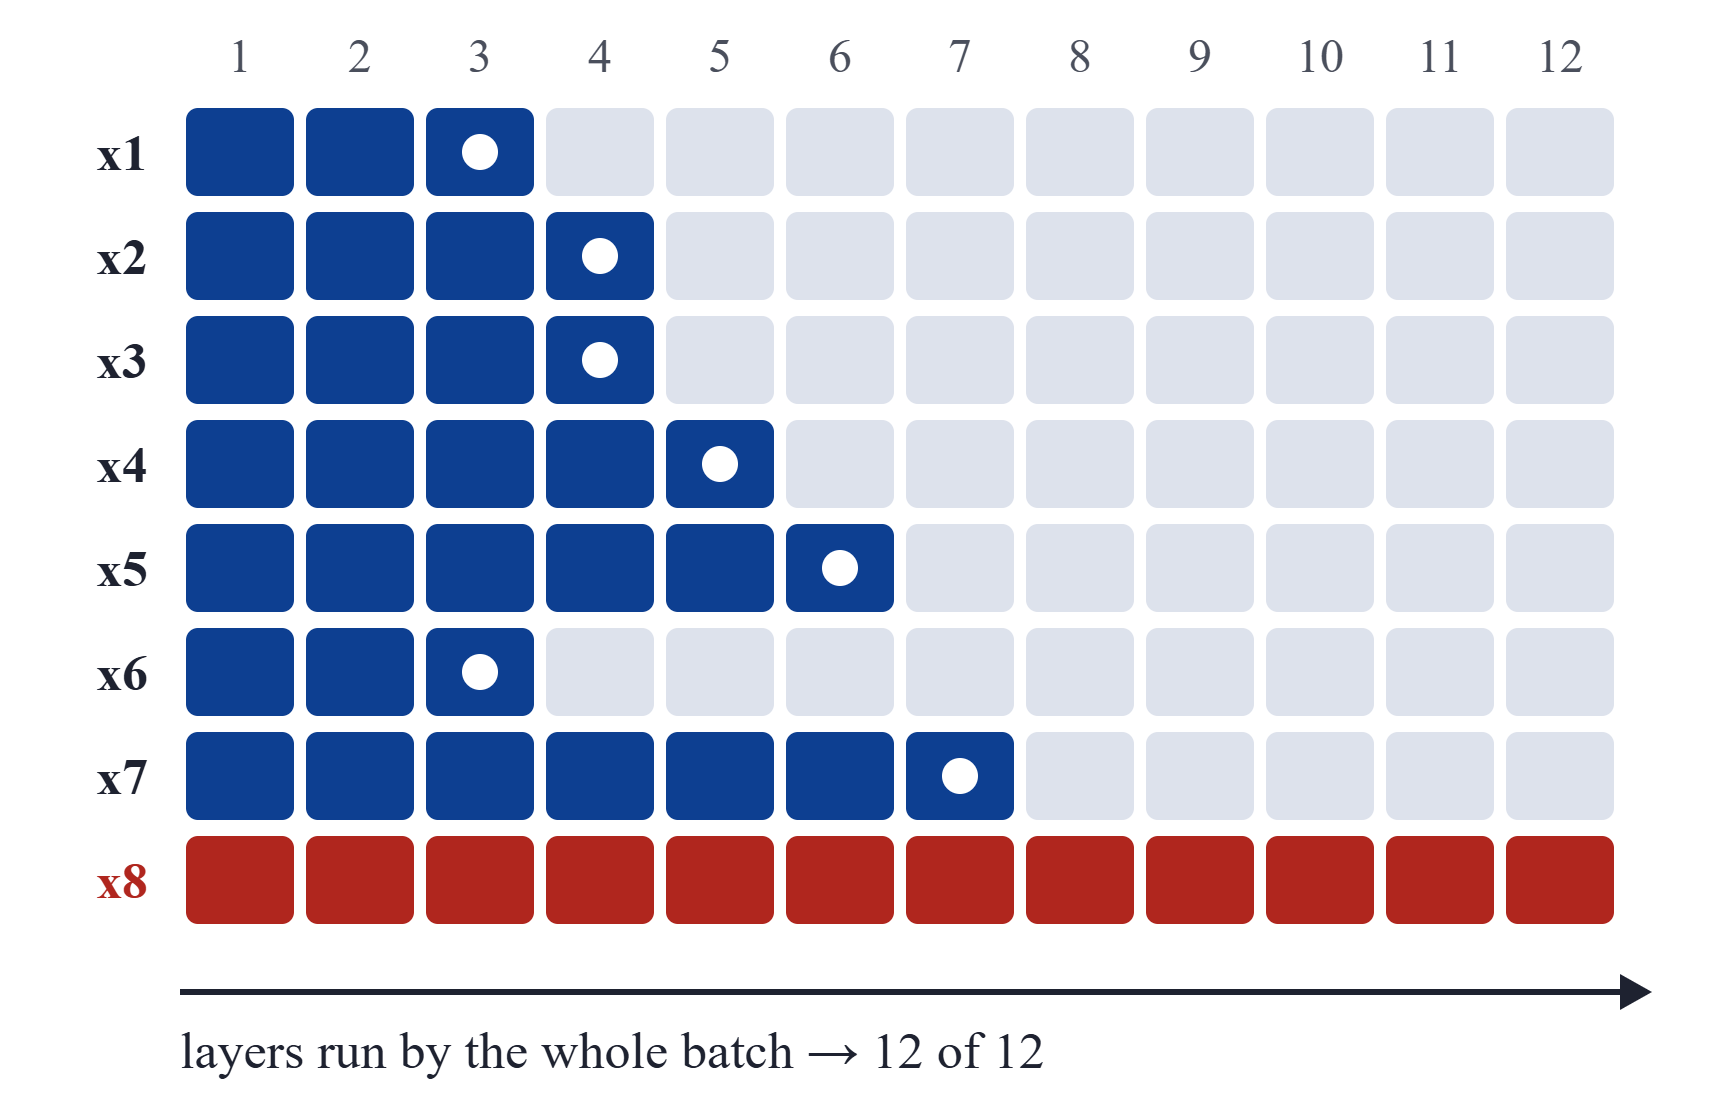
\includegraphics[width=0.62\textwidth]{fig/straggler.png}
  \caption{The straggler problem. One batch of 8 inputs through a 12-layer network. Blue: computed; grey: idle
  (the input already exited, $\circ$); red: the straggler. The mean exit is layer 5.5, yet the batch pays for all
  12 layers.}
  \label{fig:straggler}
\end{figure}

\paragraph{Cost model.} One layer run on the $n$ inputs still active costs $c(n)$. Exits sit after layers
$l_1<\dots<l_E=L$. Only a subset is evaluated, the \emph{exit plan} $S=\{s_1<\dots<s_m=E\}$, and each evaluated
exit costs $h$. Write $d_i$ for the layer of the $i$-th evaluated exit ($d_0=0$) and $n_i$ for the number of inputs
active on the layers between evaluated exits $i-1$ and $i$. If the batch ends at its $k$-th evaluated exit, its
latency is
\begin{equation}\label{eq:latency}
  T_{\text{batch}} \;=\; \sum_{i=1}^{k} \big[(d_i-d_{i-1})\,c(n_i) + h\big].
\end{equation}
Every layer up to the stopping depth is paid for, including layers whose exits are not in the plan; $h$ is paid only
for exits that are evaluated.

The first report assumed $c(n)=a+bn$ and described the regime by $\rho=a/(bn)$. When $\rho$ is small
(compute-bound), removing an exited input saves real time, so per-input exits work. When $\rho$ is large
(fixed-cost-bound), removing one input saves almost nothing and only stopping the whole batch saves time. That
picture stands, but Section~\ref{sec:cost} shows the affine form is a poor fit on a second GPU, so the method takes
the measured $c(n)$ directly.

\paragraph{Gap.} Existing batch-level rules are heuristics: Consensus waits until every input is confident, and
Majority and Greedy stop when half or one of them is~\cite{drex,miao}. None is derived from the cost. Apparate
chooses which exits to keep by their saving minus their overhead, but all inputs still run to the end of the model
and accuracy is monitored without a guarantee~\cite{apparate}. Risk-controlled early exit gives a guarantee, but for
per-input exits with no batch coupling~\cite{fastsafe}.

\paragraph{Setting, and what we do not compare against.} A batch is formed once, runs, and all its answers are
returned; the quantity of interest is the latency of that batch. The other way to deal with stragglers is to
rebatch: DREX regroups the inputs that continue past an exit into new batches with other requests waiting at that
depth, and E3 splits the model at its exits so that each part runs at a constant batch size~\cite{drex,e3}.
Rebatching needs other requests to regroup with, so it applies under sustained load; it does not apply to a fixed
offline batch, at low load, or when a batch has a latency deadline. The two are complementary, and this report has no
rebatching baseline, which is a limitation. Stopping a batch also has a cost that rebatching does not: the inputs
forced out are the hard ones, so the accuracy loss is not spread evenly. Section~\ref{sec:front} reports the loss on
hard inputs separately.

\paragraph{Security coupling.} A slowdown attacker crafts inputs that never become confident~\cite{sloth,lostpatience,falsesense}.
In a synchronous batch, such an input delays every co-batched user, not only itself.

\paragraph{Research questions.} Given the measured $c(n)$:
\begin{enumerate}
  \item When should a batch stop, and which exits are worth evaluating?
  \item Can the rule's parameters be set with a guarantee on accuracy, and learned online without labels?
  \item Can the damage from slowdown inputs be bounded without detecting them?
\end{enumerate}

% ---------------------------------------------------------------------------------------------------- 2
\section{Approach}\label{sec:approach}

\subsection{Batch-stopping rule for a measured cost}\label{sec:rule}
The objective for one batch is its mean accuracy minus $\lambda\cdot T_{\text{batch}}/F$, with $F$ the latency of
the full model at the same batch size. $\lambda$ has no unit: it is the accuracy we are willing to give up to save
one full-model latency. Let $g_j(e\to e')$ be the expected accuracy gain of carrying input $j$ from exit $e$ to a
later exit $e'$, estimated from a calibration table of $P(\text{correct at } e' \mid \text{confidence at } e)$. One
input contributes $1/B$ of the batch's mean accuracy, which is why its gain is divided by $B$. Input $j$ leaves alone
if
\begin{equation}\label{eq:indiv}
  \frac{g_j(e\to E)}{B} \;<\; \lambda\cdot\frac{[c(n)-c(n-1)]\,(L-l_e)}{F},
\end{equation}
and the remaining inputs $R$ stop together if no later evaluated exit is worth reaching:
\begin{equation}\label{eq:coll}
  \forall e'\in S,\ e'>e:\qquad \frac{1}{B}\sum_{j\in R} g_j(e\to e') \;<\;
  \lambda\cdot\frac{(l_{e'}-l_e)\,c(|R|) + m(e,e')\,h}{F},
\end{equation}
where $m(e,e')$ counts the evaluated exits after $e$ up to and including $e'$.

An individual exit saves only the marginal cost $c(n)-c(n-1)$; a collective stop saves all of $c(|R|)$. For the
affine cost these are $b$ and $a+b|R|$, which recovers the rule of the first report and its threshold ratio of about
$1/(1+\rho)$. For a cost with a floor the marginal cost is zero below the knee, so the rule switches from per-input
exits to whole-batch stopping inside a batch as it drains.

Two approximations are built in. Rule~\eqref{eq:indiv} prices the saving as if the input would otherwise run to
layer $L$ at today's marginal cost; when the batch later stops early the true saving is smaller, so~\eqref{eq:indiv}
overestimates it. Rule~\eqref{eq:coll} looks ahead to each later exit separately and uses only the current
confidences. Lookahead rules of this kind are optimal in the monotone case of optimal stopping~\cite{chow}, which
needs, among other conditions, gains that diminish with depth and a cost that is linear in $n$. On 13 November we
had not shown these conditions for a measured $c(n)$, and the floor-shaped cost of Section~\ref{sec:cost} violates
the linear one; Section~\ref{sec:theory} gives what we proved afterwards.

\subsection{Exit plan}\label{sec:plan}
The first rule evaluated every exit and paid $h$ for each. The plan $S$ is now a choice: any subset of the
intermediate exits, with the rule \eqref{eq:indiv}--\eqref{eq:coll} run on that subset. With one exit kept the plan
behaves like a unified exit; with all exits kept it is the earlier rule. The plan and $\lambda$ are chosen together
by replaying calibration traces under the measured $c(n)$ and $h$; this needs no GPU time.

\subsection{Certified selection}\label{sec:cert}
The first report chose the fastest setting whose accuracy on the tuning split was within one point of the full
model, and it then lost 0.8--2.5 points on held-out data. We now split the tuning data in two. On the first part each
method's candidates are reduced to a path ordered from safest to fastest. On the second part the path is tested in
order: for candidate $\theta$, the drop in accuracy against the full model is computed per batch on $K$ disjoint
batches, $Z_1,\dots,Z_K$, and $\theta$ is certified if a one-sided $t$-test rejects ``mean drop $>\alpha$'' at
level $\delta$. Testing stops at the first candidate that fails (fixed-sequence testing, as in
Learn-then-Test~\cite{ltt}); the fastest certified candidate is used. We use $\alpha=1$ point and $\delta=10\%$.
Batches, not inputs, are the unit, because a batch-level rule couples the inputs of a batch. The test treats the $K$
batch drops as independent draws from one distribution. That holds here because the batches are disjoint random
groups from one split, and it means the guarantee covers inputs from the same distribution only. The $t$-test is
also valid only for large $K$; Section~\ref{sec:tighten} tests finite-sample bounds. The certificate holds for the
batch size and cost it was computed for, and recomputing it for a new deployment is a replay on the CPU.

\subsection{Label-free, partial-feedback bandit (secondary)}\label{sec:bandit}
The bandit replaces ``correct'' with ``agrees with the full model'', which upper-bounds the accuracy loss. Feedback is
censored: once a batch stops, its deeper exits are never seen. Probe batches run to full depth with probability
$c\,t^{-1/3}$, the partial-monitoring rate for a revealing action~\cite{labeleff}. Prior bandits for early exit
tune per-input thresholds~\cite{ceebert,ucbee}.

\subsection{Bounded damage from slowdown inputs}\label{sec:robust}
The robust rule leaves the $m$ largest gains out of the collective sum in~\eqref{eq:coll}. A trimmed sum is
monotone, so for $k\le m$ slowdown inputs $K$ among clean inputs $C$,
\[
  TS_m(C) \;\le\; TS_m(C\cup K) \;\le\; TS_{m-k}(C), \qquad\text{hence}\qquad
  \operatorname{depth}(C\cup K;\,m) \;\le\; \operatorname{depth}(C;\,m-k)
\]
for every batch. The property is simple, and it bounds the damage without removing it: the batch can still run
deeper as $k$ grows.

\textbf{Scope of the proof.} The argument covers the collective stop~\eqref{eq:coll} with the trimmed sum, for a
fixed set of active inputs. It does not cover the per-input exits of rule~\eqref{eq:indiv}. Slowdown inputs stay in
the batch, so they change the number $n$ of active inputs and with it the marginal cost $c(n)-c(n-1)$ that decides
whether a clean input leaves. For the measured cost, which is only made non-decreasing, this marginal cost need not
be monotone in $n$, so the active set under attack is not ordered against the clean one. For the full rule the bound
is therefore an empirical property: Sections~\ref{sec:robust4} and~\ref{sec:robust5} check it on every tested batch, and that is
evidence, not a proof.

% ---------------------------------------------------------------------------------------------------- 3
\section{Experimental setup}\label{sec:setup}

\begin{table}[ht]
  \centering\small
  \resizebox{\textwidth}{!}{\begin{tabular}{@{}lllcl@{}}
    \toprule
    Model & Task & Exits after layer & Full-model acc. & Used in \\
    \midrule
    RoBERTa-base~\cite{roberta} & MNLI~\cite{mnli} & 2, 4, \dots, 12 & 87.8\% & server and local \\
    RoBERTa-base & QQP~\cite{glue} & 2, 4, \dots, 12 & 91.1\% & server and local \\
    ViT-B/16~\cite{vit} & CIFAR-100~\cite{cifar} & 2, 4, \dots, 12 & 93.3\% & server \\
    \makecell[l]{Qwen2.5-1.5B, Llama-3.1-8B\\(decoders)~\cite{qwen,llama}} & \makecell[l]{WikiText-103~\cite{wikitext}\\next token} & 6 exits & 49.9\%, 53.6\% & \makecell[l]{server\\(negative result)} \\
    \makecell[l]{Qwen2.5-1.5B,\\Llama-3.1-8B-Instruct\\(classifiers)} & MNLI, QQP & \makecell[l]{Qwen 4, 8, \dots, 28;\\Llama 8, 12, \dots, 32\\(7 exits)}
      & \makecell{Qwen 89.4, 90.1\%;\\Llama 90.9, 90.9\%} & server \\
    \bottomrule
  \end{tabular}}
  \caption{Models and tasks. Encoder backbones were fine-tuned jointly with their six exits (training details in
  Step~R\ref{st:train}). The decoders' exits were trained on a frozen backbone (13 November) and then with LoRA
  (Section~\ref{sec:llm}). The LLM classifiers train LoRA adapters (rank 16, $\alpha=32$) and one head per exit
  on the last prompt token (Step~R\ref{st:llm}); their accuracies are MNLI, QQP on the whole validation set.}
  \label{tab:models}
\end{table}

\paragraph{Server.} One RTX A6000. Three kinds of measurement were made on it, and they differ:
\begin{itemize}
  \item \textbf{Figure~\ref{fig:server}} (13 November): the trained checkpoints in fp16 on real inputs, in two
  execution modes, eager PyTorch and CUDA graphs (a compiled stack).
  \item \textbf{Tables~\ref{tab:t11}, \ref{tab:t12} and~\ref{tab:t12b}} (after 13 November): the replay method of
  the local GPU described next, that is, a random-weight fp32 network replaying the trained model's recorded
  decisions, eager only. Their first captions said ``trained checkpoint, real inputs''; that label was wrong and is
  corrected here.
  \item \textbf{Tables~\ref{tab:t15}--\ref{tab:t16}} (LLM classifiers): trained weights and real prompts, bf16,
  eager.
\end{itemize}

\paragraph{Local.} One GTX 1650 (4\,GB), fp32 (fp16 is about four times slower on this card). The trained
checkpoints are not on this machine. The timed network has the trained model's architecture and tensor shapes with
random weights; every layer, exit head, host synchronisation, batch compaction and policy call is executed and timed,
and the exit decisions and predictions are those recorded for the trained model on the same inputs. Accuracy is
therefore exact for the trained model and time is exact for this hardware. Sequence lengths 16 and 32 use decisions
recorded at length 128; they show how the same policies behave when per-input compute is smaller, and they are not a
claim about truncated inputs.

\paragraph{Protocol.} Each validation set is split in half. Parameters are chosen on the tuning half by certified
selection (Section~\ref{sec:cert}; 40\% for tables and candidate paths, 60\% for the test) and reported on the
held-out half. Local timing runs 1{,}920 held-out inputs per pass at lengths 16 and 32 (5 rounds) and 768 at length
128 (3 rounds), with policies interleaved within a round; we report the median over rounds of the paired speedup and
its range.

\paragraph{Baselines.} Per-sample threshold (DeeBERT-style), unified exit (SkipDecode-style~\cite{skipdecode}, one
head evaluated), Majority (as in DREX), a 150-trial random search over a 3-parameter collective rule, and the
per-sample threshold given the same exit-plan search as our rule (an Apparate-style selection of exits~\cite{apparate}).

% ---------------------------------------------------------------------------------------------------- 4
\section{Results up to 13 November}\label{sec:status}

This section is the ``Current status'' section of the progress report of 13 November. The cost-rule rows of
Table~\ref{tab:resplit} were regenerated on 26 November after a caching bug was fixed (Appendix~\ref{app:issues});
the 13 November values are given in brackets where they changed. Ten numbers in the 13 November text do not match
the committed result files; they are corrected here and marked with a footnote.

\subsection{Corrections to the first report}
The progress report opened its results with the claims of the first report that the new measurements
narrowed or withdrew. Table~\ref{tab:corrections} lists them with the evidence and the hardware it was measured on.
\begin{table}[H]
  \centering\small
  \begin{tabularx}{\textwidth}{@{}>{\raggedright\arraybackslash}p{4.2cm}X>{\raggedright\arraybackslash}p{2.3cm}@{}}
    \toprule
    First report said & What the evidence shows & Measured on \\
    \midrule
    The rule matches or beats the best heuristic in every cell & With CUDA graphs it is never the single fastest
      rule: unified exit wins at $B\le16$ on text, a random search ties or wins at $B\ge64$. At $B=8$ on MNLI it was
      the slowest rule (0.86\x) & Server, CUDA graphs \\
    1.41\x, 2.10\x, 1.46\x{} at $B=64$ within one accuracy point & Those were simulated and selected on the held-out
      split. The real-GPU runs lost 0.8--2.5 points on held-out data & Server, eager \\
    The simulator tracks the GPU within about 5\% & Only at $B\ge64$ in eager mode; at $B\le16$ off by 1--47\%
      depending on the policy\footnotemark, and it overestimates in graph mode & Server, both modes \\
    Every collective rule beats per-sample exits at $B\le16$ & True on MNLI and QQP, not on CIFAR-100 & Server, ViT \\
    Robustness costs no clean speedup & True at high $\rho$. At low $\rho$ on CIFAR-100 the robust rule reaches
      1.24\x{} against 1.46\x\footnotemark & Server, ViT \\
    Tuned parameters carry over between deployments (assumed) & Tested and false for every method: in simulation the
      rule broke the one-point budget in 29--31\% of transfers & Simulation, 3 tasks \\
    \bottomrule
  \end{tabularx}
  \caption{Claims of the first report that were narrowed or withdrawn.}
  \label{tab:corrections}
\end{table}
\addtocounter{footnote}{-1}%
\corrtext{the 13 November text said ``15--32\% off''. How that aggregate was computed was not recorded, and it cannot
be traced to a result file; the per-policy errors at $B\le16$ in the result files are 1--47\%.}%
\stepcounter{footnote}%
\corrtext{the 13 November text said 1.12\x; the committed result file is a 22 November rerun and gives 1.24\x.}

\subsection{No rule wins everywhere, and the winner flips with the deployment (server)}\label{sec:server}
\begin{figure}[ht]
  \centering
  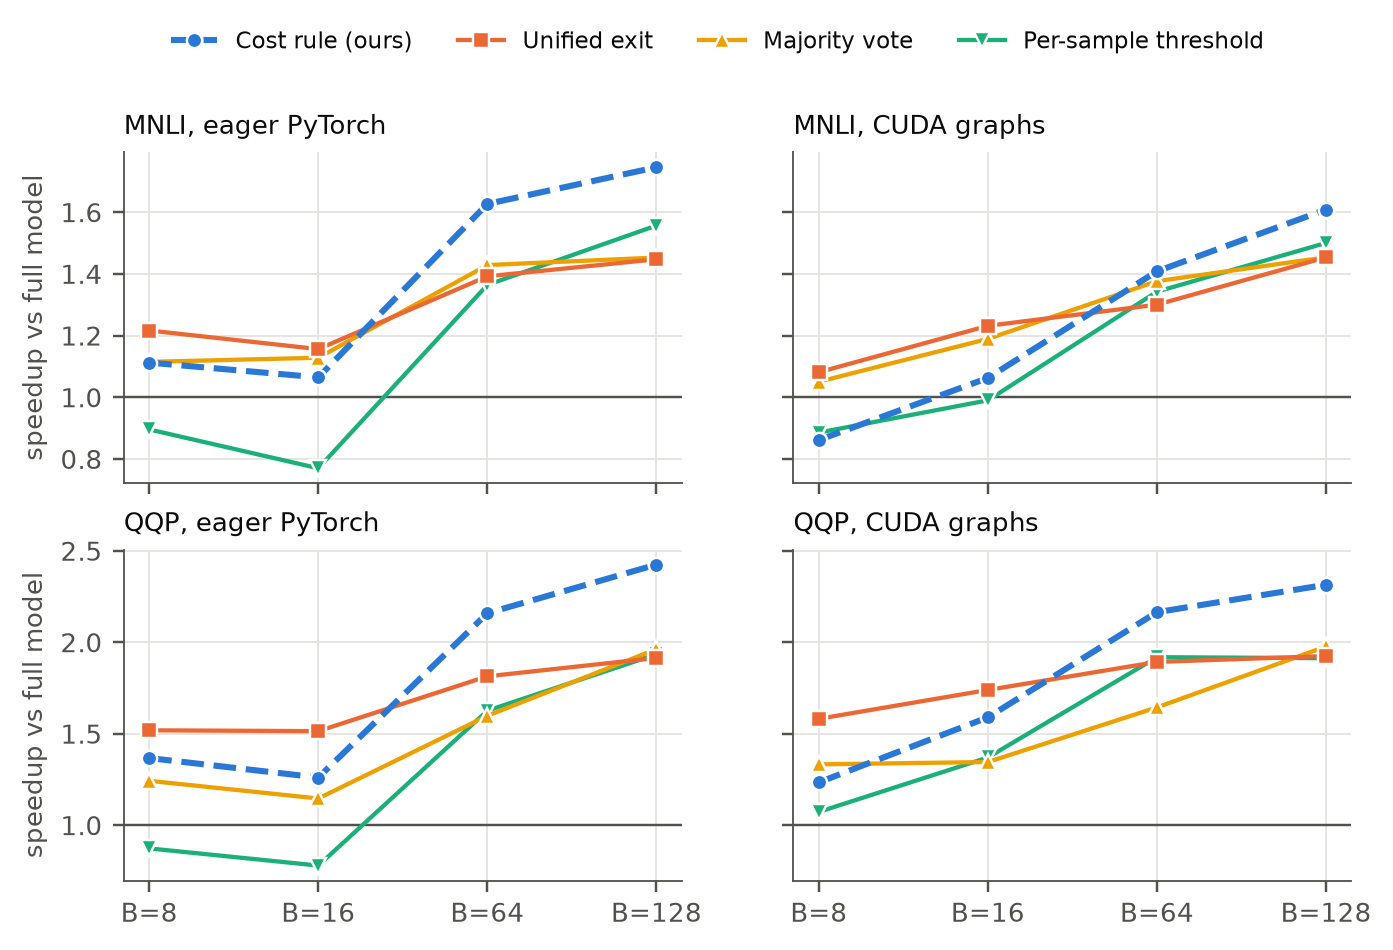
\includegraphics[width=0.92\textwidth]{fig/report2_server_speedups.png}
  \caption{Real wall-clock speedup against the full model on an RTX A6000, held-out split. Left: eager PyTorch.
  Right: CUDA graphs. These runs used the old selection protocol and are not accuracy-matched (on MNLI the cost rule
  lost 1.8--2.5 points, unified exit 0.8--0.9); Section~\ref{sec:server-cert} reruns them with certified selection.}
  \label{fig:server}
\end{figure}

Figure~\ref{fig:server} shows the server measurements. Three statements hold in both execution modes. Wait-for-all
early exit, which keeps exited inputs in the batch, is slower than no early exit (0.78--0.97\x). Per-sample exits fall
below 1\x{} at small batches on text (0.77--0.90\x{} eager, 0.89\x{} on MNLI with CUDA graphs). And the ordering of
rules changes between $B=8$ and $B=128$. Compiling cuts the fixed per-layer cost about six-fold, and the cause of the
small-batch loss changes with it: under CUDA graphs it is the exit heads, which alone cost 19\% of the runtime at
$B=8$ on MNLI (12\% on QQP).\corr{the 13 November text gave 19\% for both tasks; it is 19\% on MNLI and 12\% on QQP.}

\subsection{The cost is a floor followed by a linear part (GTX 1650)}\label{sec:cost}
\begin{figure}[ht]
  \centering
  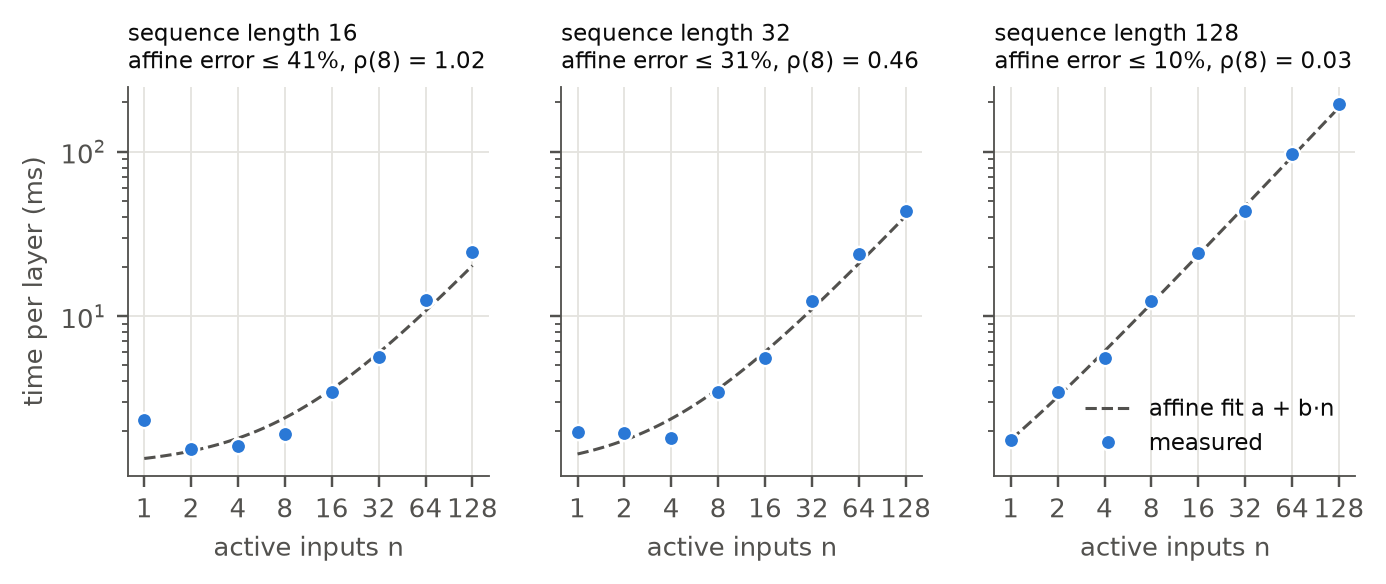
\includegraphics[width=0.92\textwidth]{fig/report2_cost_gtx1650.png}
  \caption{Measured time of one RoBERTa-base layer on a GTX 1650 (fp32) against the number of active inputs, at
  three sequence lengths, with the affine fit of the first report. Both axes are logarithmic.}
  \label{fig:cost}
\end{figure}

\begin{table}[ht]
  \centering\small
  \begin{tabular}{@{}lccccccc@{}}
    \toprule
    Sequence length & $c(1)$ ms & $c(8)$ ms & $c(64)$ ms & $h$ ms & $\rho$ at $n=8$ & $\rho$ at $n=64$ & \makecell{Affine fit,\\largest error} \\
    \midrule
    16  & 2.32 & 1.92  & 12.48 & 0.42 & 1.02 & 0.127 & 41\% \\
    32  & 1.97 & 3.46  & 24.00 & 0.42 & 0.46 & 0.058 & 31\% \\
    128 & 1.76 & 12.35 & 97.23 & 0.52 & 0.03 & 0.003 & 10\% \\
    \bottomrule
  \end{tabular}
  \caption{Per-layer cost and exit-head cost on the GTX 1650. File: \file{results/local\_cost\_cuda\_T\{16,32,128\}.json}.}
  \label{tab:cost}
\end{table}

A layer costs about 1.8\,ms however few inputs are active, and then grows in proportion to the number of tokens in
the batch. The knee is near 128 tokens: one input at length 128, four at length 32, eight at length 16. The affine
model is off by up to 41\% at short sequences. One GPU therefore covers both regimes: at length 128 it is
compute-bound at every batch size, and at length 16 with $B=8$ a per-input exit saves nothing. Policies below are
chosen with the measured table. The gain in predicting speedups is small, because a speedup is a ratio and errors
partly cancel: over the 126 policy runs timed in Section~\ref{sec:local} the table's median error is 1.3\% (largest
17\%), against 2.2\% (largest 15\%) for the affine fit applied to the same decisions. The floor matters for the
rule's decisions more than for the prediction.

\subsection{Exit plan and certified selection, real wall-clock (GTX 1650)}\label{sec:local}
\begin{figure}[ht]
  \centering
  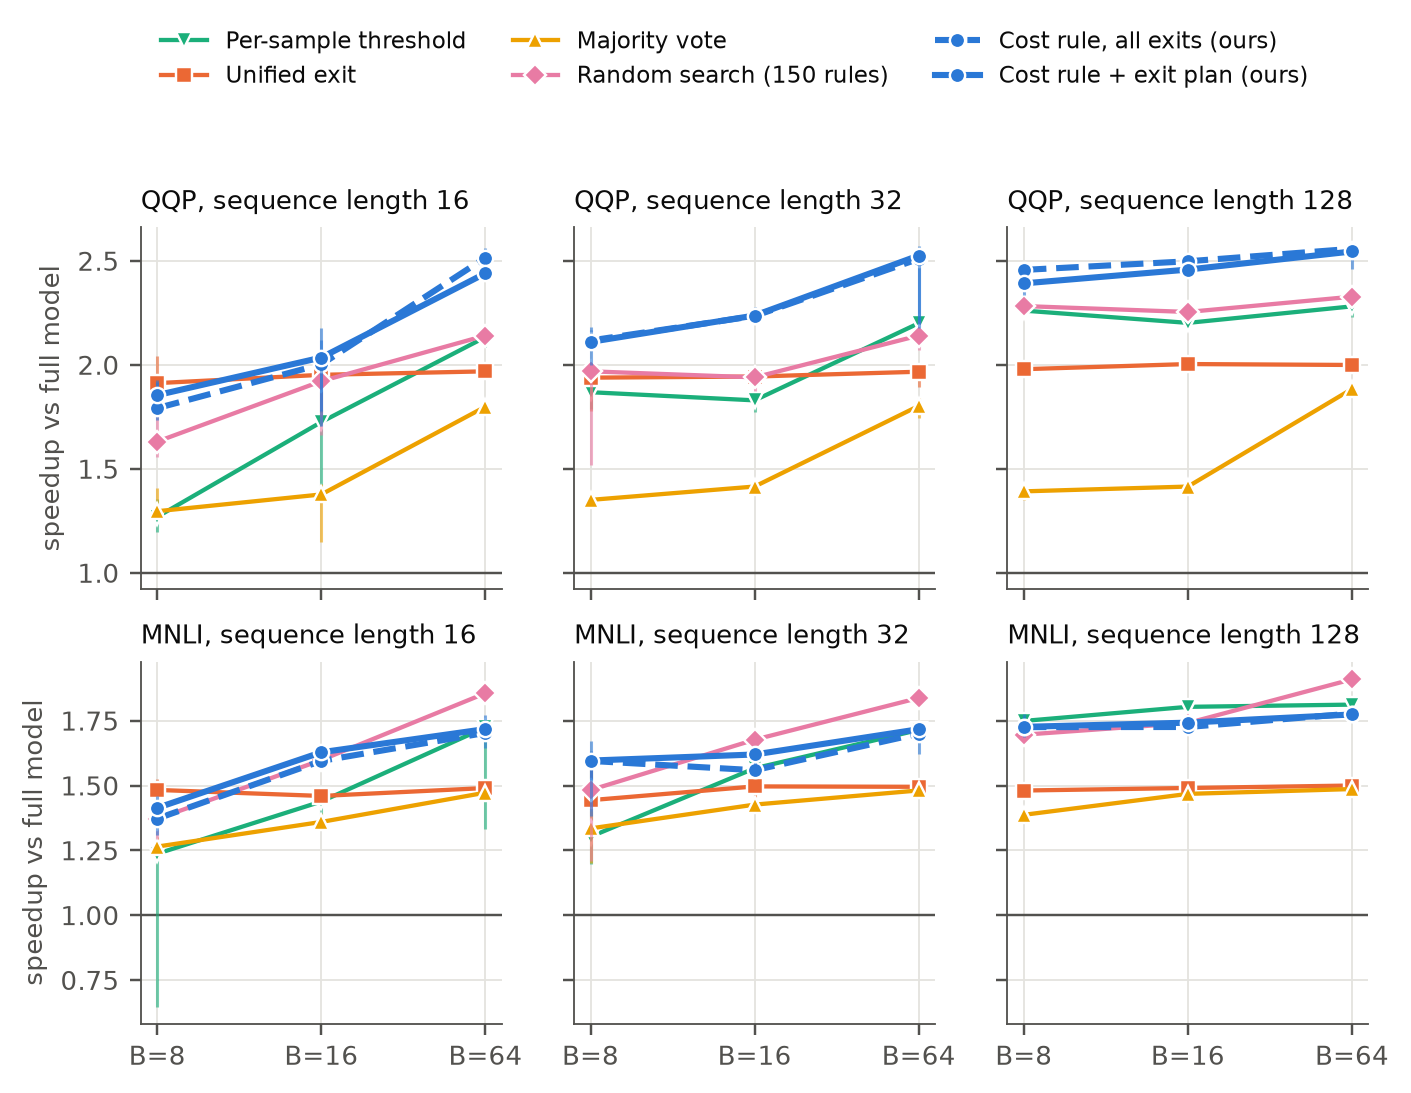
\includegraphics[width=0.86\textwidth]{fig/report2_local_speedups.png}
  \caption{Real wall-clock speedup on the GTX 1650 of the certified policy of each method, held-out inputs. Markers
  are the median over rounds; vertical bars are the range. Dashed blue: the cost rule with all exits; solid blue:
  with an exit plan.}
  \label{fig:local}
\end{figure}

\begin{table}[ht]
  \centering\footnotesize\setlength{\tabcolsep}{4pt}
  \begin{tabular}{@{}lccccccccc@{}}
\toprule
 & \multicolumn{3}{c}{sequence length 16} & \multicolumn{3}{c}{sequence length 32} & \multicolumn{3}{c}{sequence length 128} \\
\cmidrule(lr){2-4}\cmidrule(lr){5-7}\cmidrule(lr){8-10}
Policy & $B=8$ & $B=16$ & $B=64$ & $B=8$ & $B=16$ & $B=64$ & $B=8$ & $B=16$ & $B=64$ \\
\midrule
All heads, no exits & 0.93 & 0.96 & 0.99 & 0.96 & 0.97 & 0.99 & 0.99 & 0.99 & 1.00 \\
\midrule
Per-sample threshold & 1.27 & 1.73 & 2.13 & 1.87 & 1.83 & 2.20 & 2.26 & 2.20 & 2.28 \\
Threshold + exit plan & 1.86$^{*}$ & 1.92$^{*}$ & 2.15 & 1.93$^{*}$ & 1.90 & 2.19 & 2.27 & 2.20 & 2.30 \\
Unified exit & \textbf{1.91}$^{*}$ & 1.95$^{*}$ & 1.97$^{*}$ & 1.94$^{*}$ & 1.94$^{*}$ & 1.97$^{*}$ & 1.98$^{*}$ & 2.00$^{*}$ & 2.00$^{*}$ \\
Majority vote & 1.30 & 1.38 & 1.80 & 1.35 & 1.42 & 1.80 & 1.39 & 1.42 & 1.88 \\
Random search (150 rules) & 1.63 & 1.92 & 2.14 & 1.97 & 1.94 & 2.14 & 2.28 & 2.25 & 2.33 \\
\midrule
Cost rule, all exits \textit{(ours)} & 1.79 & 2.00 & \textbf{2.52} & \textbf{2.12} & \textbf{2.24} & 2.51 & \textbf{2.46} & \textbf{2.50} & \textbf{2.56} \\
Cost rule + exit plan \textit{(ours)} & 1.85 & \textbf{2.04} & 2.44 & 2.11 & \textbf{2.24} & \textbf{2.53} & 2.39 & 2.46 & 2.55 \\
\bottomrule
\end{tabular}

  \caption{QQP, GTX 1650, measured speedup of each method's certified policy. Bold: fastest in the column.
  $^{*}$ held-out accuracy drop above one point. File: \file{results/local\_time\_qqp\_cuda\_T\{16,32,128\}.csv}.}
  \label{tab:t04}
\end{table}

\begin{table}[ht]
  \centering\footnotesize\setlength{\tabcolsep}{4pt}
  \begin{tabular}{@{}lccccccccc@{}}
\toprule
 & \multicolumn{3}{c}{sequence length 16} & \multicolumn{3}{c}{sequence length 32} & \multicolumn{3}{c}{sequence length 128} \\
\cmidrule(lr){2-4}\cmidrule(lr){5-7}\cmidrule(lr){8-10}
Policy & $B=8$ & $B=16$ & $B=64$ & $B=8$ & $B=16$ & $B=64$ & $B=8$ & $B=16$ & $B=64$ \\
\midrule
All heads, no exits & 0.93 & 0.96 & 0.98 & 0.95 & 0.98 & 0.99 & 0.98 & 0.98 & 1.00 \\
\midrule
Per-sample threshold & 1.24$^{*}$ & 1.44$^{*}$ & 1.72$^{*}$ & 1.30$^{*}$ & 1.57$^{*}$ & 1.71$^{*}$ & \textbf{1.75}$^{*}$ & \textbf{1.80}$^{*}$ & 1.81$^{*}$ \\
Threshold + exit plan & 1.46 & 1.45 & 1.63 & 1.47 & 1.48 & 1.68 & 1.67 & 1.72 & 1.77 \\
Unified exit & \textbf{1.48} & 1.46 & 1.49 & 1.44 & 1.50 & 1.50 & 1.48 & 1.49 & 1.50 \\
Majority vote & 1.26$^{*}$ & 1.36 & 1.47 & 1.33$^{*}$ & 1.43 & 1.48 & 1.39$^{*}$ & 1.47 & 1.49 \\
Random search (150 rules) & 1.37 & 1.60$^{*}$ & \textbf{1.86}$^{*}$ & 1.48 & \textbf{1.68}$^{*}$ & \textbf{1.84}$^{*}$ & 1.70 & 1.74 & \textbf{1.91}$^{*}$ \\
\midrule
Cost rule, all exits \textit{(ours)} & 1.37$^{*}$ & 1.60$^{*}$ & 1.70$^{*}$ & \textbf{1.60}$^{*}$ & 1.56$^{*}$ & 1.70$^{*}$ & 1.73$^{*}$ & 1.73$^{*}$ & 1.78 \\
Cost rule + exit plan \textit{(ours)} & 1.41 & \textbf{1.63}$^{*}$ & 1.72$^{*}$ & \textbf{1.60}$^{*}$ & 1.62$^{*}$ & 1.72$^{*}$ & 1.73$^{*}$ & 1.74$^{*}$ & 1.77 \\
\bottomrule
\end{tabular}

  \caption{MNLI, same layout. File: \file{results/local\_time\_mnli\_cuda\_T\{16,32,128\}.csv}.}
  \label{tab:t05}
\end{table}

\begin{table}[ht]
  \centering\footnotesize
  \resizebox{\textwidth}{!}{\begin{tabular}{@{}lccccc@{}}
    \toprule
    Policy & \makecell{Mean speed rel.\\to the cell's best} & Worst cell & \makecell{Cells within\\3\% of the best}
      & \makecell{Cells over the 1-pt\\budget (held-out)} & \makecell{Largest held-out\\drop (pts)} \\
    \midrule
    Per-sample threshold        & 0.884 & 0.664 & 2 / 18  & 9 / 18 & 1.23 \\
    Threshold + exit plan       & 0.912 & 0.848 & 2 / 18  & 3 / 18 & 1.05 \\
    Unified exit                & 0.859 & 0.779 & 2 / 18  & 9 / 18 & 1.05 \\
    Majority vote               & 0.738 & 0.566 & 0 / 18  & 3 / 18 & 1.20 \\
    Random search (150 rules)   & 0.934 & 0.848 & 5 / 18  & 5 / 18 & 1.44 \\
    Cost rule, all exits (ours) & 0.970 & 0.917 & 11 / 18 & 8 / 18 & 1.31 \\
    Cost rule + exit plan (ours)& 0.975 & 0.925 & 11 / 18 & 7 / 18 & 1.28 \\
    \bottomrule
  \end{tabular}}
  \caption{Summary over 2 tasks \x{} 3 batch sizes \x{} 3 sequence lengths (18 timed cells; lengths 16 and 32 change
  the timing only, Section~\ref{sec:setup}). Speed is relative to the fastest method of each cell. The methods are
  not at the same accuracy here: the fifth column differs by method, so this table is not a ranking.
  Section~\ref{sec:front} compares speed at matched accuracy.}
  \label{tab:summary}
\end{table}

Tables~\ref{tab:t04}--\ref{tab:summary} and Figure~\ref{fig:local} give the measurements. What they show:
\begin{itemize}
  \item \textbf{The regime flip reproduces on this GPU.} On QQP at sequence length 16 and $B=8$, the per-sample
  threshold reaches 1.27\x{} and a unified exit 1.91\x; at $B=64$ the threshold reaches 2.13\x{} and the unified exit
  1.97\x. At sequence length 128, where the GPU is compute-bound at every batch size, the threshold is ahead of the
  unified exit throughout.
  \item \textbf{The cost rule is close to the fastest method in every timed cell, but not at equal accuracy.} With
  an exit plan it is at most 7.5\% behind (MNLI, $B=64$, behind the random search) and within 3\% of the fastest in
  11 of 18 settings. The best baselines by this measure, the random search and the threshold with an exit plan, are
  15\% behind in their worst setting; the unified exit 22\%; the per-sample threshold 34\%; majority vote 43\%. These
  policies do not sit at the same held-out accuracy: the rule is over one point in 7 of 18 cells, majority vote and
  the threshold with a plan in 3. The numbers in this item are therefore not a ranking; Section~\ref{sec:front}
  compares the methods at matched accuracy.
  \item \textbf{On QQP} one of the rule's two variants is the fastest in eight of nine settings (2.52\x{} against
  2.15\x{} for the next method at length 16 and $B=64$, with ranges that do not overlap) and 3\% behind the unified
  exit in the ninth. Its held-out drop with a plan is 0.52--0.82 points.
  \item \textbf{On MNLI it is not the fastest.} A unified exit is 5\% ahead at length 16 and $B=8$, and the random
  search is 7--8\% ahead at $B=64$, as it was on the server.
  \item \textbf{The exit plan helps only a little here.} It raises the rule from 1.79\x{} to 1.85\x{} (QQP) and from
  1.37\x{} to 1.41\x{} (MNLI) at length 16 and $B=8$, and changes little elsewhere: on this GPU the five exit heads
  cost at most 7\% of the runtime. The plan's real test is the server under CUDA graphs, where they cost 19\%.
  \item \textbf{The accuracy budget is not met on MNLI's held-out half.} Policies were certified at one point on the
  tuning half, yet on the held-out half the rule with a plan loses 0.88--1.28 points (7 of 9 MNLI settings above one
  point), the per-sample threshold 1.21--1.23 in all nine, and the random search up to 1.44. On QQP the unified exit
  lands at 1.05 points in all nine settings. Every method shifts by a similar amount on MNLI, which suggests the two
  4{,}900-example halves differ; Section~\ref{sec:resplit} tests the procedure on random re-splits.
\end{itemize}
\textbf{Limits of this experiment.} Decisions are replayed from recorded traces on a randomly initialised network
(Section~\ref{sec:setup}); 12 of the 18 cells are the same recorded decisions timed at a shorter sequence length, so
the independent workloads are 2 tasks \x{} 3 batch sizes; one GPU; three to five timing rounds per setting, so a range
is shown and not a confidence interval. At $B=16$ and length 16 one noisy round widens the ranges and the top four
methods are tied there.

\subsection{Speed at matched accuracy, and where the accuracy loss lands (cost table, GTX 1650)}\label{sec:front}
\begin{figure}[ht]
  \centering
  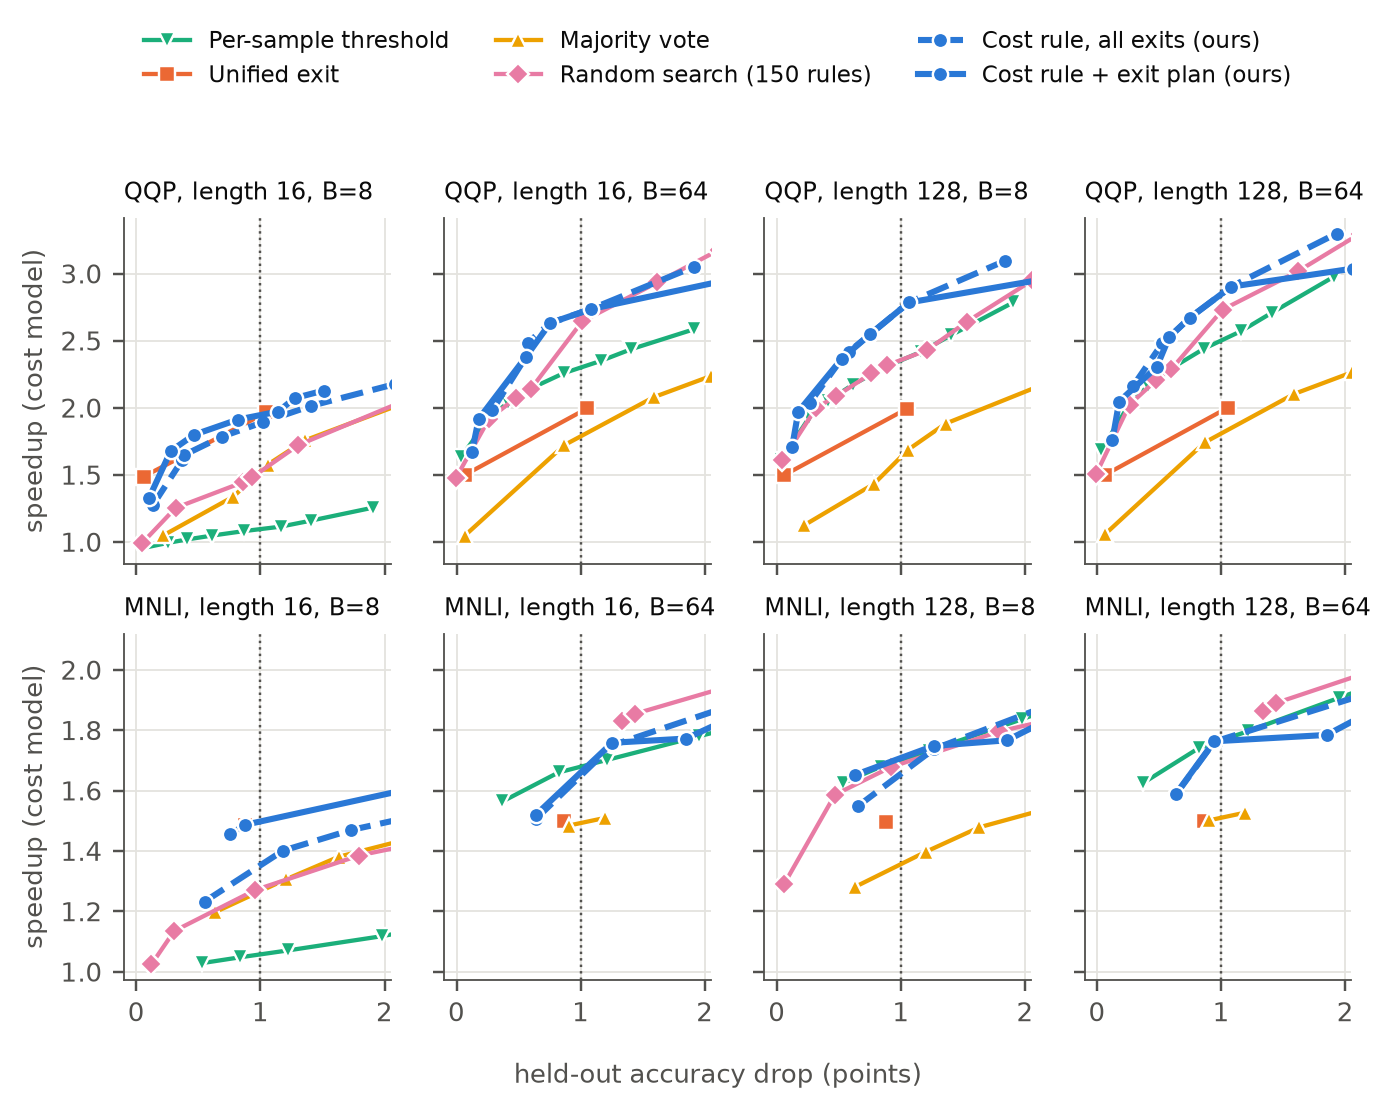
\includegraphics[width=0.82\textwidth]{fig/report2_front.png}
  \caption{Held-out accuracy drop against speedup. Each point is the policy that certified selection returns for one
  accuracy target between 0.25 and 3 points, scored once on the held-out half. Up and to the left is better. The
  dotted line is the one-point budget. Speedups are computed from the measured cost table, not timed.}
  \label{fig:front}
\end{figure}

\begin{table}[ht]
  \centering\small
  \begin{subtable}{\textwidth}\centering
    \begin{tabular}{@{}lcccccc@{}}
\toprule
 & \multicolumn{3}{c}{sequence length 16} & \multicolumn{3}{c}{sequence length 128} \\
\cmidrule(lr){2-4}\cmidrule(lr){5-7}
Policy & $B=8$ & $B=16$ & $B=64$ & $B=8$ & $B=16$ & $B=64$ \\
\midrule
Per-sample threshold & 1.08 & 1.48 & 2.26 & 2.30 & 2.32 & 2.44 \\
Threshold + exit plan & 1.88 & 1.89 & 2.16 & 2.26 & 2.29 & 2.35 \\
Unified exit & 1.49 & 1.49 & 1.50 & 1.50 & 1.50 & 1.50 \\
Majority vote & 1.34 & 1.45 & 1.72 & 1.43 & 1.51 & 1.74 \\
Random search (150 rules) & 1.48 & 1.89 & 2.14 & 2.32 & 2.36 & 2.29 \\
\midrule
Cost rule, all exits \textit{(ours)} & 1.78 & \textbf{2.13} & \textbf{2.63} & \textbf{2.55} & \textbf{2.48} & \textbf{2.67} \\
Cost rule + exit plan \textit{(ours)} & \textbf{1.91} & 2.08 & \textbf{2.63} & \textbf{2.55} & \textbf{2.48} & \textbf{2.67} \\
\bottomrule
\end{tabular}

    \caption{QQP. File: \file{results/local\_front\_qqp\_cuda\_T\{16,128\}.csv}.}\label{tab:t07}
  \end{subtable}\par\medskip
  \begin{subtable}{\textwidth}\centering
    \begin{tabular}{@{}lcccccc@{}}
\toprule
 & \multicolumn{3}{c}{sequence length 16} & \multicolumn{3}{c}{sequence length 128} \\
\cmidrule(lr){2-4}\cmidrule(lr){5-7}
Policy & $B=8$ & $B=16$ & $B=64$ & $B=8$ & $B=16$ & $B=64$ \\
\midrule
Per-sample threshold & 1.05 & 1.30 & \textbf{1.66} & \textbf{1.68} & 1.68 & 1.74 \\
Threshold + exit plan & 1.48 & 1.49 & 1.63 & 1.67 & 1.68 & 1.72 \\
Unified exit & \textbf{1.49} & 1.49 & 1.50 & 1.50 & 1.50 & 1.50 \\
Majority vote & 1.20 & 1.41 & 1.48 & 1.28 & 1.47 & 1.50 \\
Random search (150 rules) & 1.27 & 1.38 & -- & \textbf{1.68} & \textbf{1.69} & -- \\
\midrule
Cost rule, all exits \textit{(ours)} & 1.23 & 1.48 & 1.51 & 1.55 & 1.58 & \textbf{1.76} \\
Cost rule + exit plan \textit{(ours)} & \textbf{1.49} & \textbf{1.52} & 1.52 & 1.65 & -- & \textbf{1.76} \\
\bottomrule
\end{tabular}

    \caption{MNLI. File: \file{results/local\_front\_mnli\_cuda\_T\{16,128\}.csv}.}\label{tab:t08}
  \end{subtable}
  \caption{Speedup of each method's fastest policy whose held-out drop is at most one point (cost table, GTX 1650).
  Bold: best in the column. --: no such policy. (Tables 7 and 8 of the progress report.)}
  \label{tab:matched}
\end{table}

\begin{table}[ht]
  \centering\scriptsize\setlength{\tabcolsep}{3pt}
  \begin{tabular}{@{}lcccccccccccc@{}}
    \toprule
    & \multicolumn{3}{c}{QQP, length 16} & \multicolumn{3}{c}{QQP, length 128} & \multicolumn{3}{c}{MNLI, length 16} & \multicolumn{3}{c}{MNLI, length 128} \\
    \cmidrule(lr){2-4}\cmidrule(lr){5-7}\cmidrule(lr){8-10}\cmidrule(lr){11-13}
    Policy & all & hard 25\% & other & all & hard 25\% & other & all & hard 25\% & other & all & hard 25\% & other \\
    \midrule
    Per-sample threshold         & 0.61 & 1.03 & 0.47 & 0.61 & 1.03 & 0.47 & 1.22 & 0.57 & 1.44 & 1.22 & 0.57 & 1.44 \\
    Threshold + exit plan        & 0.90 & 3.06 & 0.18 & 0.61 & 1.03 & 0.47 & 0.89 & 2.07 & 0.50 & 0.97 & 0.57 & 1.10 \\
    Unified exit                 & 1.05 & 4.08 & 0.04 & 1.05 & 4.08 & 0.04 & 0.87 & 2.75 & 0.24 & 0.87 & 2.75 & 0.24 \\
    Majority vote                & 0.78 & 2.73 & 0.13 & 0.78 & 2.73 & 0.13 & 1.01 & 2.86 & 0.39 & 1.01 & 2.86 & 0.39 \\
    Random search (150 rules)    & 0.70 & 1.85 & 0.31 & 0.66 & 1.23 & 0.46 & 1.15 & 1.69 & 0.97 & 1.08 & 1.28 & 1.01 \\
    Cost rule, all exits (ours)  & 0.61 & 1.58 & 0.28 & 0.58 & 1.29 & 0.35 & 1.23 & 2.70 & 0.75 & 1.12 & 2.01 & 0.83 \\
    Cost rule + exit plan (ours) & 0.74 & 2.04 & 0.31 & 0.57 & 1.27 & 0.33 & 1.12 & 2.59 & 0.63 & 1.12 & 2.01 & 0.83 \\
    \bottomrule
  \end{tabular}
  \caption{Held-out accuracy drop in points at the one-point target, mean over $B=8,16,64$: all inputs, the hard
  quarter (lowest mean confidence over the five intermediate exits), and the rest. The rows of the threshold, the
  unified exit and majority vote are the same at both lengths because their certified parameters do not change with
  the cost table.}
  \label{tab:hard}
\end{table}

Tables~\ref{tab:t04}--\ref{tab:summary} compare one policy per method, and those policies differ in accuracy. Here
each method is run through certified selection at eight accuracy targets, which traces its accuracy--speed front on
held-out data (Figure~\ref{fig:front}). Table~\ref{tab:matched} reads each front at a held-out drop of at most one
point. Speedups in this section come from the measured cost table; over the timed runs of Section~\ref{sec:local}
the table's median error was 1.3\% and its largest 17\%.
\begin{itemize}
  \item \textbf{QQP:} the rule is ahead in all six settings, by 2--17\% over the best baseline (2.63\x{} against
  2.26\x{} at length 16 and $B=64$; 2.55\x{} against 2.32\x{} at length 128 and $B=8$).
  \item \textbf{MNLI: no advantage.} The rule is within 2\% of the best baseline in four of six settings and behind
  in two: 8.5\% behind the per-sample threshold at length 16 and $B=64$, and 6.5\% behind the random search at length
  128 and $B=16$. At length 128, where the GPU is compute-bound, the per-sample threshold is as fast as any
  batch-level rule.
  \item \textbf{The exit plan matters at small batches on the cost floor.} At length 16 and $B=8$ the rule without a
  plan reaches 1.23\x{} on MNLI and 1.78\x{} on QQP; with a plan, 1.49\x{} and 1.91\x. The threshold gains as much
  from the same plan search (1.05\x{} to 1.48\x{} on MNLI). On MNLI at this setting the plan keeps a single
  intermediate exit (layer 8) and is the same policy as the unified exit (both 1.49\x).
  \item \textbf{Why the plan variant is sometimes behind the rule with all exits.} The plan search uses every second
  value of $\lambda$, so it does not contain every all-exits policy, and selection on the tuning half can return a
  slower or a less accurate policy. The ``--'' in Table~\ref{tab:t08} arises this way: at length 128 and $B=16$ the
  selected plan policy has a held-out drop of 1.16 points at every target up to 2 points, so it has no point within
  one point.
  \item \textbf{What the derivation buys, and what it does not.} The rule without a plan has one parameter and 40
  candidates; the random search has three parameters and 150 candidates. With the plan search the rule has 620
  candidates, more than any baseline; the closest is the threshold with a plan (558). In five of the six QQP settings the rule
  without a plan is already ahead, so the lead there is not bought with a larger search. At length 16 and $B=8$ only
  the plan variant is ahead (1.91\x{} against 1.88\x{} for the threshold with a plan; 1.78\x{} without a plan), and
  the plan variant is not a cheaper search than the baselines. It does not buy transfer between deployments
  (Table~\ref{tab:corrections}). Whether it needs less calibration data is tested in Section~\ref{sec:tighten}.
  \item \textbf{The accuracy loss lands on hard inputs} (Table~\ref{tab:hard}). At the one-point target the rule
  loses 2.0--2.7 points on the hard quarter of MNLI and 1.3--2.0 on QQP, against 0.6 and 1.0 for the per-sample
  threshold. On MNLI the threshold takes its loss from the easier inputs (1.4 points on the other three quarters); on
  QQP its hard quarter also loses more than the rest (1.0 against 0.5). A unified exit is the most uneven (2.8 and
  4.1 points). This is a cost of any rule that stops a batch, ours included, and the one-point average hides it.
\end{itemize}
\textbf{Limits.} Speedups are from the cost table, not timed. Each front has at most eight points, and reading it at
``at most one point'' picks among them on held-out data, the same way for every method. MNLI's held-out half is
4{,}900 examples, so a difference of a few percent between two methods there is within noise we have not measured.

\subsection{Does the certificate hold on re-splits?}\label{sec:resplit}
\begin{table}[ht]
  \centering\footnotesize\setlength{\tabcolsep}{3.5pt}
  \begin{tabular}{@{}lllcccccc@{}}
    \toprule
    & & & \multicolumn{2}{c}{Over budget} & \multicolumn{2}{c}{Mean drop (pts)} & \multicolumn{2}{c}{Speedup (cost model)} \\
    \cmidrule(lr){4-5}\cmidrule(lr){6-7}\cmidrule(lr){8-9}
    Task & $B$ & Policy & old protocol & certified & old & certified & old & certified \\
    \midrule
    MNLI & 8  & Majority vote        & 33\% & 10\% & 0.87 & 0.43 & 1.36\x & 1.23\x \\
    MNLI & 8  & Cost rule, all exits & 40\% & 3\% [7\%] & 0.85 [0.83] & 0.36 [0.35] & 1.45\x & 1.33\x \\
    MNLI & 8  & Per-sample threshold & 40\% & 7\%  & 0.90 & 0.59 & 1.06\x & 1.04\x \\
    MNLI & 64 & Majority vote        & 40\% & 13\% & 0.88 & 0.43 & 1.52\x & 1.29\x \\
    MNLI & 64 & Cost rule, all exits & 47\% [37\%] & 3\% [0\%] & 0.96 [0.99] & 0.34 [0.33] & 1.80\x & 1.55\x{} [1.59\x] \\
    MNLI & 64 & Per-sample threshold & 43\% & 10\% & 0.88 & 0.56 & 1.69\x & 1.64\x \\
    QQP  & 8  & Majority vote        & 27\% & 7\%  & 0.76 & 0.62 & 1.42\x & 1.33\x \\
    QQP  & 8  & Cost rule, all exits & 33\% [13\%] & 0\% & 0.90 [0.84] & 0.61 [0.62] & 1.90\x{} [1.88\x] & 1.79\x{} [1.80\x] \\
    QQP  & 8  & Per-sample threshold & 3\%  & 0\%  & 0.85 & 0.72 & 1.09\x & 1.07\x \\
    QQP  & 64 & Majority vote        & 3\%  & 3\%  & 0.74 & 0.56 & 1.75\x & 1.56\x \\
    QQP  & 64 & Cost rule, all exits & 23\% [13\%] & 0\% [3\%] & 0.90 [0.73] & 0.64 & 2.68\x{} [2.60\x] & 2.52\x{} [2.54\x] \\
    QQP  & 64 & Per-sample threshold & 3\%  & 0\%  & 0.85 & 0.72 & 2.26\x & 2.20\x \\
    \bottomrule
  \end{tabular}
  \caption{Share of 30 random re-splits (20\% tables and paths, 30\% certification, 50\% test) whose test-half
  accuracy drop exceeds one point, sequence length 16. Speedups here are from the cost model, not from GPU timing.
  Cost-rule rows after the 26 November cache fix; [13 November value] where it changed. File:
  \file{results/local\_resplit\_\{qqp,mnli\}\_cuda\_T16.csv}.}
  \label{tab:resplit}
\end{table}

On random re-splits the certified procedure keeps the budget. For the cost rule the test half is over one point in
0--3\% of re-splits, against 23--47\% for the old protocol; the mean drop is 0.34--0.64 points.\corr{these figures
were 0--7\%, 13--40\% and 0.33--0.64 before the cache fix of 26 November; the price in speed was 2--4\% on QQP and
8--12\% on MNLI, and the old protocol's MNLI range 33--43\%.} Eleven of the twelve rows are at or below the 10\%
target; majority vote on MNLI at $B=64$ is at 13\% (4 of 30), which 30 re-splits cannot separate from 10\%. The price
is speed: about 6\% on QQP and 9--14\% on MNLI for the cost rule. It is larger on MNLI, whose tuning half has about
4{,}900 examples against about 20{,}200 for QQP, so the test needs a wider margin there. The old protocol went over
budget in 33--47\% of MNLI re-splits for every method. Its mean drop on re-splits is 0.7--1.0 points, so this explains
how often the earlier runs broke the budget; it does not explain the largest losses of the first report (up to 2.5
points). This also bears on Section~\ref{sec:local}: the fixed MNLI held-out half, where most certified policies
exceeded one point, behaves like one of the unlucky splits and not like the average one. That reading is consistent
with these numbers but is not proved by them, and a 30-re-split estimate of a 10\% rate is coarse.

\subsection{Secondary: the label-free bandit (server, single seeds)}
Against an oracle that knows the true tables, cumulative regret over 3{,}000 batches of 64 grows with a log--log
slope of 0.49--0.65 on MNLI and QQP,\corr{these single-run slopes are not in the repository; the committed files hold
a later 3-seed run, whose refit gives 0.56--0.63. Section~\ref{sec:bandit10} replaces both with ten seeds.} while a
CeeBERT-style per-input bandit's regret grows linearly. On the GPU the bandit uses no labels, costs 0.2--0.3 accuracy
points, and reaches 1.26--1.77\x{} at $B=64$--128. Two cautions that the first report did not state: these are single
runs fitted on a few points, and a slope below 2/3 does not ``confirm'' the $T^{2/3}$ rate, which is a worst-case
bound.

\subsection{Bounded damage from slowdown inputs (server)}\label{sec:robust4}
The bound $\operatorname{depth}(C\cup K;m)\le\operatorname{depth}(C;m-k)$ held in all 10{,}500 batches tested on
five task--model pairs (MNLI, QQP and CIFAR-100, and WikiText-103 next-token prediction on Qwen2.5-1.5B and on
Llama-3.1-8B), including real DeepSloth inputs on the ViT; on the other tasks the slowdown inputs are the hardest
natural inputs, not crafted attacks. For the full rule this is an empirical check, not a consequence of the proof
of Section~\ref{sec:robust}; the property test passes on the local machine as well (19 of
19 unit tests). Consensus loses its whole speedup to a single attacker on CIFAR-100 (DeepSloth inputs); on MNLI and
QQP its latency rises from 0.70 to 0.74 and from 0.72 to 0.85 of the full model at $k=1$, and it collapses at
$k=8$.\corr{the 13 November text said consensus loses its whole speedup to a single attacker on every task.} Victims'
latency under our rule still rises with $k$, and the robust rule has a clean-speed cost in the low-$\rho$ regime
(Table~\ref{tab:corrections}).

\subsection{What did not work}\label{sec:negative}
\begin{itemize}
  \item \textbf{A faster rule at a fixed setting.} Random search, program search (FunSearch-style~\cite{funsearch}, 300 programs),
  trajectory-aware calibration and a hindsight-best batch depth all tie the rule. A hidden-state probe adds at most
  0.026 AUROC over confidence. The limit is the exit signal, not the stopping rule.
  \item \textbf{Decoders.} The cost model holds on Qwen2.5-1.5B and Llama-3.1-8B, but exits are too weak: at 75\%
  depth frozen Llama heads are 8.2 points short of the full model and public LayerSkip checkpoints~\cite{layerskip}
  4.9 and 5.2 points short,\corr{the 13 November text said ``both about 5 points short''; the frozen Llama heads are
  8.2 points short (layer 24 of 32).} and no rule beats the full model within one point.
  \item \textbf{Transfer of tuned parameters.} See Table~\ref{tab:corrections}. This is why selection is redone per
  deployment with a certificate, which costs a CPU replay.
  \item \textbf{Straggler rescue} brought no measurable gain.
\end{itemize}

% ---------------------------------------------------------------------------------------------------- 5
\section{Results of the planned work (13--26 November)}\label{sec:planned}

The progress report ended with a plan (its Section 5). Each item below states what we planned, what we expected and
the fallback, as written on 13 November, followed by the result. All numbers are on held-out data with a one-point
accuracy budget.

\subsection{Accuracy-matched server tables with the exit plan}\label{sec:server-cert}
\textit{Plan.} Rerun the 24 server settings (3 tasks \x{} 4 batch sizes \x{} eager and CUDA graphs) with the exit
plan, the measured cost table and certified selection, and report each as a timed accuracy--speed front.
\textit{Expected:} at a matched drop of one point, the rule ahead on QQP and within 10\% of the best baseline
elsewhere. \textit{Fallback:} if it is more than 10\% behind at $B\le16$ under CUDA graphs, report the plan as a
partial fix and state the settings where a unified exit should be used.

\textbf{Result (16--25 Nov, eager only; partial, 9 of 24 settings).} Run for QQP and MNLI at sequence lengths 128 and
32 (Tables~\ref{tab:t11}--\ref{tab:t12}). CUDA graphs and CIFAR-100 needed a working A6000; on 23--24 November none
could start CUDA, and the ViT run of 25 November got through $B=8$ only (Table~\ref{tab:t12b}). The CUDA-graph run
was not done. On QQP at length 128 the cost rule with the exit plan is the fastest policy within budget at every
batch size, 1.95--2.46\x{} at a held-out drop of 0.60--0.66 points, 8--14\% ahead of the best baseline within budget.
At length 32 and $B\le16$ the plan's policy is 0.05 points over budget (so is the unified exit's), and the rule with
all exits is the fastest policy within budget (1.30--1.33\x). On MNLI at length 128 the cost rule is over budget at
every batch size (held-out drop 1.23--1.28 points), and so are the per-sample threshold (1.21--1.25 points) and, at
$B\ge16$, random search (1.06--1.48 points). The fastest policies within budget there are the unified exit, the threshold with an exit
plan and majority vote, at 1.46--1.66\x. At length 32 and $B\le16$ the plan's policy is within budget but 3--5\%
behind the unified exit. On CIFAR-100 at $B=8$ the rule with the plan (1.44\x) is 2.8\% behind the threshold with a
plan (1.48\x), both within budget.

\begin{table}[ht]
  \centering\footnotesize\setlength{\tabcolsep}{4pt}
  \begin{tabular}{@{}lcccccccc@{}}
\toprule
 & \multicolumn{4}{c}{QQP, length 128} & \multicolumn{4}{c}{QQP, length 32} \\
\cmidrule(lr){2-5}\cmidrule(lr){6-9}
Policy & $B=8$ & $B=16$ & $B=64$ & $B=128$ & $B=8$ & $B=16$ & $B=64$ & $B=128$ \\
\midrule
Per-sample threshold & 1.48 & 1.79 & 2.11 & 2.13 & 0.84 & 0.85 & 1.75 & 2.03 \\
Threshold + exit plan & 1.90$^{*}$ & 1.83 & 2.15 & 2.13 & 1.73$^{*}$ & 1.80$^{*}$ & 1.86 & 2.04 \\
Unified exit & 1.91$^{*}$ & 1.96$^{*}$ & 1.99$^{*}$ & 1.99$^{*}$ & 1.79$^{*}$ & 1.83$^{*}$ & 1.97$^{*}$ & 1.98$^{*}$ \\
Majority vote & 1.33 & 1.40 & 1.80 & 1.87 & 1.06 & 1.16 & 1.73 & 1.83 \\
Random search (150 rules) & 1.77 & 1.99 & 2.11 & 2.26 & 1.09 & 1.14 & 1.75 & 2.34 \\
\midrule
Cost rule, all exits \textit{(ours)} & 1.84 & \textbf{2.20} & 2.45 & 2.39 & \textbf{1.33} & \textbf{1.30} & \textbf{2.11} & \textbf{2.37} \\
Cost rule + exit plan \textit{(ours)} & \textbf{1.95} & \textbf{2.20} & \textbf{2.46} & \textbf{2.44} & 1.68$^{*}$ & 1.76$^{*}$ & \textbf{2.11} & 2.30 \\
\bottomrule
\end{tabular}

  \caption{QQP, RTX A6000, eager PyTorch: measured speedup of each method's certified policy on held-out inputs
  (2{,}048 per pass, 5 rounds, median paired speedup). Decisions of the trained RoBERTa-base model replayed on a
  random-weight fp32 network. Bold: fastest policy within the one-point budget in the column. $^{*}$ held-out drop
  above one point. File: \file{results/local\_time\_qqp\_a6000\_T\{128,32\}.csv}.}
  \label{tab:t11}
\end{table}

\begin{table}[ht]
  \centering\footnotesize\setlength{\tabcolsep}{4pt}
  \begin{tabular}{@{}lcccccccc@{}}
\toprule
 & \multicolumn{4}{c}{MNLI, length 128} & \multicolumn{4}{c}{MNLI, length 32} \\
\cmidrule(lr){2-5}\cmidrule(lr){6-9}
Policy & $B=8$ & $B=16$ & $B=64$ & $B=128$ & $B=8$ & $B=16$ & $B=64$ & $B=128$ \\
\midrule
Per-sample threshold & 1.33$^{*}$ & 1.54$^{*}$ & 1.69$^{*}$ & 1.73$^{*}$ & 0.85$^{*}$ & 0.93$^{*}$ & 1.48$^{*}$ & 1.65$^{*}$ \\
Threshold + exit plan & \textbf{1.46} & \textbf{1.51} & \textbf{1.66} & 1.67$^{*}$ & 1.38 & 1.41 & 1.47 & 1.63$^{*}$ \\
Unified exit & \textbf{1.46} & 1.49 & 1.50 & 1.50 & \textbf{1.42} & \textbf{1.45} & \textbf{1.48} & \textbf{1.49} \\
Majority vote & 1.32$^{*}$ & 1.40 & 1.48 & \textbf{1.51} & 1.05$^{*}$ & 1.20 & 1.44 & \textbf{1.49} \\
Random search (150 rules) & 1.44 & 1.66$^{*}$ & 1.80$^{*}$ & 1.83$^{*}$ & 1.01 & 1.22$^{*}$ & 1.71$^{*}$ & 1.79$^{*}$ \\
\midrule
Cost rule, all exits \textit{(ours)} & 1.47$^{*}$ & 1.63$^{*}$ & 1.72$^{*}$ & 1.71$^{*}$ & 1.07 & 1.20$^{*}$ & 1.61$^{*}$ & 1.67$^{*}$ \\
Cost rule + exit plan \textit{(ours)} & 1.54$^{*}$ & 1.65$^{*}$ & 1.71$^{*}$ & 1.72$^{*}$ & 1.35 & 1.40 & 1.65$^{*}$ & 1.69$^{*}$ \\
\bottomrule
\end{tabular}

  \caption{MNLI, same layout. File: \file{results/local\_time\_mnli\_a6000\_T\{128,32\}.csv}.}
  \label{tab:t12}
\end{table}

\begin{table}[ht]
  \centering\footnotesize
  \begin{tabular}{@{}lc@{}}
\toprule
 & \multicolumn{1}{c}{eager} \\
\cmidrule(lr){2-2}
Policy & $B=8$ \\
\midrule
Per-sample threshold & 1.46 \\
Threshold + exit plan & \textbf{1.48} \\
Unified exit & -- \\
Majority vote & 1.00 \\
Random search (150 rules) & 1.46 \\
\midrule
Cost rule, all exits \textit{(ours)} & 1.40 \\
Cost rule + exit plan \textit{(ours)} & 1.44 \\
\bottomrule
\end{tabular}

  \caption{CIFAR-100, ViT-B/16 (197 tokens), RTX A6000, same protocol, timed only at $B=8$ (eager): the 25 November
  run stopped during $B=16$. File: \file{results/local\_time\_cifar100\_a6000\_T197.csv}.}
  \label{tab:t12b}
\end{table}

\subsection{Tighten the certificate}\label{sec:tighten}
\textit{Plan.} Replace the $t$-test with a finite-sample bound for bounded batch losses (Hoeffding--Bentkus~\cite{rcps}), add
the label-free version that controls disagreement with the full model, and repeat the re-split check on CIFAR-100.
In the same runs, repeat the selection with 10\%, 25\% and 50\% of the calibration data for the cost rule and for
the random search. \textit{Expected:} the same violation rates with a speed cost of a few percent.
\textit{Fallback:} keep the $t$-test and state it as an asymptotic guarantee with the measured violation rate.

\textbf{Result (Table~\ref{tab:cert}; outcome = fallback).} The $t$-test keeps the share of re-splits over budget at
or below $\delta=10\%$ on average on all three tasks (1.5\% QQP, 5.2\% MNLI, 8.5\% CIFAR-100, mean over five methods).
On CIFAR-100 two methods are slightly above $\delta$ (per-sample threshold 13.3\%, cost rule + plan 12.5\%), which
120 cases per method cannot separate from 10\% (the 95\% interval is about $\pm5$ points). The finite-sample bounds
are too conservative at these sample sizes: for the accuracy drop, Hoeffding--Bentkus certifies no policy on any
task, and the Waudby-Smith--Ramdas (WSR) betting bound~\cite{wsr} certifies one in 49\% of the QQP cases, at 1.51\x{} against 2.31\x{} with the $t$-test, and
never on MNLI or CIFAR-100. The label-free version (disagreement with the full model) had no violations and costs
speed: 1.88\x{} against 2.31\x{} on QQP. With 10\% of the calibration data the cost rule falls from 2.32\x{} to
1.66\x{} on QQP, and random search loses less ($-20\%$ against $-28\%$: 2.13\x{} $\to$ 1.71\x), so the
data-efficiency hypothesis (one parameter needs less data than three) is not supported. We therefore state the
certificate as asymptotic, checked on re-splits.

\textbf{The MNLI held-out half} (A6000 cost table, length 128, the policies of Table~\ref{tab:t12}). On the fixed
split three methods exceed the budget at $\delta=10\%$: the cost rule (1.23--1.28 points with or without the plan),
the per-sample threshold (1.21--1.25) and, at $B\ge16$, random search (1.06--1.48). The unified exit and the
threshold with an exit plan stay at or just above it (0.86--1.01 points). At $\delta=2\%$ the cost rule is within budget at $B\le64$
(0.47--0.80 points) for 10--13\% less speed, but not at $B=128$ (1.25). On 30 random re-splits at $\delta=10\%$ the
cost rule is over budget in 5.8\% of cases. Lowering $\delta$ to 5\% cuts that to 2.5\% (with the plan 7.5\% $\to$
3.3\%, random search 4.2\% $\to$ 0.8\%) for about 2\% less speed (1.50\x{} $\to$ 1.47\x). We read the fixed-split
overshoot as an unlucky split, not a distribution shift; these numbers are consistent with that reading and do not
prove it.

\begin{table}[ht]
  \centering\scriptsize\setlength{\tabcolsep}{3pt}
  \resizebox{\textwidth}{!}{\begin{tabular}{@{}llcccccc@{}}
    \toprule
    Task & \makecell[l]{$t$-test: share over budget,\\mean of 5 methods (worst)} & \makecell{Cost rule + plan,\\$t$-test (over budget)}
      & \makecell{Same, WSR bound\\(cases certified)} & \makecell{Hoeffding--\\Bentkus} & \makecell{Cost rule + plan,\\label-free $t$-test}
      & \makecell{Cost rule, all $\to$ 10\%\\of calibration data} \\
    \midrule
    QQP  & 1.5\% (2.5\%, random search) & 2.31\x{} (1.7\%) & 1.51\x{} (49\%) & never & 1.88\x{} (0.0\%) & 2.32\x{} $\to$ 1.66\x{} (1.7\%) \\
    MNLI & 5.2\% (8.3\%, threshold) & 1.50\x{} (7.5\%) & 1.00\x{} (0\%) & never & 1.28\x{} (0.0\%) & 1.50\x{} $\to$ 1.14\x{} (10.0\%) \\
    CIFAR-100 & 8.5\% (13.3\%, threshold) & 1.27\x{} (12.5\%) & 1.00\x{} (0\%) & never & 1.19\x{} (0.0\%) & 1.19\x{} $\to$ 1.00\x{} (5.8\%) \\
    MNLI, $\delta=5\%$ & 2.2\% (4.2\%, threshold) & 1.46\x{} (3.3\%) & -- & -- & 1.26\x{} (0.0\%) & 1.47\x{} $\to$ 1.08\x{} (5.0\%) \\
    \bottomrule
  \end{tabular}}
  \caption{Certified selection on 30 random re-splits of the validation traces (20\% tables and paths, 30\%
  certification, 50\% test) at $B=8,16,64,128$: share of the 120 cases per method whose test drop exceeds one point,
  and mean speedup from the cost table (not timed). $\delta=10\%$ unless stated. Values after the 26 November cache
  fix. File: \file{results/cert\_check\_\{qqp,mnli,cifar100,mnli\_d05\}\_summary.csv}.}
  \label{tab:cert}
\end{table}

\subsection{Fluctuating load}\label{sec:load}
\textit{Plan.} Replay an arrival trace in which the batch size moves between 1 and 128. Compare the rule,
re-certified for each batch size from one set of calibration traces, against heuristics tuned at a single batch size
and against heuristics re-tuned per batch size. \textit{Expected:} within 5\% of per-batch-size re-tuned heuristics
and ahead of heuristics tuned once. \textit{Fallback:} if tuned-once heuristics are as good, drop the load claim.

\textbf{Result (Table~\ref{tab:load}).} Passes on QQP: the cost rule tuned once reaches 2.32\x{} against 2.11\x{} for
the best baseline re-tuned per batch size (random search). CIFAR-100 passes only with the exit plan (1.39\x{} against
1.38\x); with all exits the rule reaches 1.24\x{} and is behind the best tuned-once baseline. MNLI fails on the
budget: tuned once, the cost rule loses 1.48 points (with the plan 1.23), and $\delta=5\%$ does not change the policy
tuned at $B=64$.

\begin{table}[ht]
  \centering\footnotesize\setlength{\tabcolsep}{3pt}
  \resizebox{\textwidth}{!}{\begin{tabular}{@{}lccccc@{}}
    \toprule
    Task & \makecell{Cost rule, tuned once\\at $B=64$ (drop)} & \makecell{Cost rule + plan,\\tuned once (drop)}
      & \makecell{Best baseline re-tuned per\\batch size, within budget} & \makecell{Best baseline tuned once,\\within budget} & Criterion \\
    \midrule
    QQP  & 2.32\x{} (0.61) & 2.31\x{} (0.62) & 2.11\x{} (random search, 0.68) & 2.10\x{} (random search once@8, 0.76) & pass \\
    MNLI & 1.68\x{} (1.48$^{*}$) & 1.67\x{} (1.23$^{*}$) & 1.63\x{} (threshold + plan, 0.97) & 1.60\x{} (threshold + plan once@64, 0.98) & fail \\
    MNLI, $\delta=5\%$ & 1.68\x{} (1.48$^{*}$) & 1.67\x{} (1.23$^{*}$) & 1.63\x{} (threshold + plan, 0.97) & 1.60\x{} (threshold + plan once@64, 0.98) & fail \\
    CIFAR-100 & 1.24\x{} (0.49) & 1.39\x{} (0.75) & 1.38\x{} (threshold + plan, 0.68) & 1.33\x{} (threshold once@8, 0.81) & pass (plan only) \\
    \bottomrule
  \end{tabular}}
  \caption{Fluctuating load: 3 arrival traces of 3{,}000 batches with $B$ from 1 to 128, throughput speedup over all
  batches and accuracy drop over all served inputs (held-out, cost-table replay). Criterion: tuned once, within
  budget, within 5\% of the best per-batch-size re-tuned baseline and ahead of every tuned-once baseline.
  $^{*}$ over the one-point budget. File: \file{results/load\_trace\_\{qqp,mnli,mnli\_d05,cifar100\}\_levels.csv}.}
  \label{tab:load}
\end{table}

\subsection{Bandit with error bars}\label{sec:bandit10}
\textit{Plan.} Ten seeds with confidence bands, a probe-rate ablation ($t^{-1/2}$, $t^{-1/3}$, constant), and a
warm start from a small labelled set. \textit{Expected:} slopes between 0.5 and 0.7 where the oracle stops batches.
\textit{Fallback:} report the measured slopes without a rate claim.

\textbf{Result} (ten seeds, $B=64$, 3{,}000 batches; \file{results/bandit\_slopes\_*\_10seeds.csv}). The log--log
slope of cumulative regret is 0.55--0.77 in the 5 settings where the bandit has regret to measure (95\% intervals
$\pm$0.01--0.03); in the remaining one (CIFAR-100, decoder cost profile) cumulative regret stays below 0.06 and the
slope means nothing. Four of the five slopes are in the 0.5--0.7 band we expected; a slope is not a proof of a rate.
The fifth, MNLI with the A6000 cost profile, is $0.77\pm0.03$, and QQP with the same profile is $0.67\pm0.03$. Both
are at or above the exponent $2/3$ of the worst-case $T^{2/3}$ rate, so on MNLI the regret grew faster than that rate
over these 3{,}000 batches. Two explanations fit and we cannot separate them. The horizon may be too short for the
asymptotic regime. Or our bandit, which plays the cost rule with optimistic gains on 12 confidence bins, may not
attain the rate at all: it is not the algorithm analysed in~\cite{labeleff}, and we have no regret bound for it. We
therefore claim sublinear regret on these runs and no rate. The $t^{-1/3}$ probe schedule has the lowest regret of
the three schedules in 3 of these 5 settings; $t^{-1/2}$ is lower in the others. The warm start reduces regret by
2--12\%.

\subsection{Robustness in the compute-bound regime}\label{sec:robust5}
\textit{Plan.} Run the attack experiments where majority vote loses its clean speedup, and test an attacker that
uses $k>m$ inputs. \textit{Expected:} the bound holds; the clean-speed cost at low $\rho$ is quantified per task.
\textit{Fallback:} claim only the certificate.

\textbf{Result} (3 tasks \x{} 4 cost profiles, $B=64$, certified tuning). The slowdown inputs are DeepSloth images
on CIFAR-100 and the hardest 2\% of natural held-out inputs on MNLI and QQP (Step~R\ref{st:robust}). The pathwise
bound held in all 25{,}200 checked batches (0 violations); for the full rule, with its per-input exits, this is
empirical (Section~\ref{sec:robust}). Two different ratios appear below, and we name each one.
\begin{itemize}
  \item \textbf{Victims' latency relative to the full model} (lower is better; 1\x{} means no saving). Collective rules
  that count votes collapse: on the text tasks majority vote reaches 1.01--1.11\x{} at 16--32 attackers and consensus
  0.97--1.10\x{} at 8. The cost rule degrades smoothly: 0.60--0.85\x{} at 32 attackers without trimming. The
  per-sample threshold is also robust (0.74--0.94\x{} at 32 attackers, outside the decoder-cost profile where it gives
  no speedup at all).
  \item \textbf{Clean speedup} (no attackers; higher is better). Trimming buys little and can cost a lot. At 32
  attackers the trimmed rules give the victims no lower latency than the untrimmed one on the text tasks, and on
  CIFAR-100 trimming eight gains cuts the clean speedup to 0.91--1.02\x{} from 1.15--1.57\x{} untrimmed.
\end{itemize}
On MNLI the certified cost rule is again over budget on the held-out half (1.4--1.6 points).

\subsection{Trained checkpoints on the local GPU}
\textit{Plan.} Repeat Section~\ref{sec:local} with the trained weights and real tokenised inputs. \textbf{Result:
not run.} The replayed-decision results stand, labelled as such (the fallback).

\subsection{LLMs: decoders (second attempt) and batched classifiers}\label{sec:llm}
\textit{Plan.} The first attempt failed for reasons we could name: the backbone was frozen while its exits were
trained, LayerSkip checkpoints are trained for drafting and not for returning the early answer, the test was run
only at batch sizes 16 and 64, and the budget was one point of next-token accuracy on free text. The second attempt
trains LoRA~\cite{lora} adapters and exit heads together with self-distillation from the final layer on Qwen2.5-1.5B, keeps a
frozen baseline at the same budget, and sweeps batch sizes from 2 to 64. \textit{Key--value cache:} a token that
exits at layer $l$ leaves the layers above it without keys and values; our decoding loop handles this the way
CALM~\cite{calm} does, projecting the exit hidden state into the keys and values of every skipped layer (about 2\% of
a layer per skipped layer). \textit{Alternative considered:} self-speculative decoding as in
LayerSkip~\cite{layerskip}, with the draft depth chosen per batch from the measured $c(n)$; not started.
\textit{Expected:} the exit at layer 24 within about 2 points of the full model (4.0 with a frozen
backbone\corr{the ``Expected'' paragraph of 13 November quoted 5.6 points here; the result file and the result
paragraph give 4.0. It also called this exit the ``75\%-depth exit'': that is true for Llama (layer 24 of 32), but
on Qwen2.5-1.5B layer 24 of 28 is at 86\% depth.}), and a speedup at small batch sizes. \textit{Fallback:} if the exit stays more than 4 points
short, the LLM track ends as a negative result with its cause.

\textbf{Result, decoding (15--16 Nov): negative.} Training the exits with LoRA narrows the gap of frozen exits
(Qwen2.5-1.5B, layer 24 of 28: 2.4 points below the fine-tuned model against 4.0 frozen), but on free-text
next-token prediction a batch-level rule has almost nothing to adapt to. We compared one adaptive rule, a
whole-batch stop at the first exit where the batch's mean confidence reaches a threshold, with a fixed exit, both
tuned to a one-point budget, in a replay on recorded traces that assumes a pure fixed per-layer cost ($b=0$, so the
latency is the depth). Its gain over the fixed exit falls from 12\% at $B=1$ to 0.2\% at $B=64$
(\file{results/adaptivity\_vs\_batch.csv}). This is one rule under one cost assumption, not timed, and not a bound
on every adaptive rule. The reason it shrinks is general, though: with random batching the batch mean confidence
has a standard deviation of about $\sigma/\sqrt{B}$, so at large $B$ every batch looks alike.

\textbf{Result, the LLM as a batched classifier (16--22 Nov, Tables~\ref{tab:t15}--\ref{tab:t16}): positive.} The
prompt is run once (prefill) and the label is read from the hidden state of the last prompt token by a small head
after each exit layer; nothing is decoded. On Llama-3.1-8B (compute-bound: $\rho=0.09$ at $B=8$) the cost rule is the
fastest policy within budget at every batch size on both tasks: QQP 3.48--3.66\x{} against 3.11--3.50\x{} (5--13\%
ahead), MNLI 2.97--3.14\x{} against 2.56--2.66\x{} (14--18\% ahead), at held-out drops of 0.42--0.44 and 0.70--0.74
points. On Qwen2.5-1.5B QQP it is 5--16\% ahead (2.18--3.02\x). Qwen2.5-1.5B MNLI is the exception: with all exits
the rule is the slowest certified policy (1.10--1.19\x); with the exit plan it reaches 1.38--1.48\x{} at a 0.2-point
drop, ahead of the best baseline within budget at $B=16,128$ (+1\%, +5\%) and behind at $B=8,64$ ($-7\%$, $-6\%$).
The per-sample threshold is faster there (1.34--1.94\x) but over budget (1.21--1.23 points). The device's predictions
agree with the recorded traces on 97--100\% of inputs at every exit.

\begin{table}[ht]
  \centering\footnotesize\setlength{\tabcolsep}{4pt}
  \begin{tabular}{@{}lcccccccc@{}}
\toprule
 & \multicolumn{4}{c}{Llama-3.1-8B} & \multicolumn{4}{c}{Qwen2.5-1.5B} \\
\cmidrule(lr){2-5}\cmidrule(lr){6-9}
Policy & $B=8$ & $B=16$ & $B=64$ & $B=128$ & $B=8$ & $B=16$ & $B=64$ & $B=128$ \\
\midrule
Per-sample threshold & 3.08 & 3.07 & 3.32 & 3.32 & 1.52 & 1.97 & 2.54 & 2.58 \\
Threshold + exit plan & 3.04 & 3.03 & 3.27 & 3.26 & 2.00 & 2.00 & 2.55 & 2.58 \\
Unified exit & 2.65 & 2.66 & 2.66 & 2.66 & 1.73 & 1.74 & 1.75 & 1.75 \\
Majority vote & 1.94 & 1.64 & 1.81 & 1.66 & 1.45 & 1.60 & 1.90 & 1.86 \\
Random search (150 rules) & 3.13 & 3.11 & 3.50 & 3.43 & 2.02$^{*}$ & 2.41 & 2.56 & 2.60 \\
\midrule
Cost rule, all exits \textit{(ours)} & \textbf{3.48} & \textbf{3.52} & \textbf{3.66} & \textbf{3.62} & 2.15 & \textbf{2.52} & \textbf{2.96} & \textbf{3.02} \\
Cost rule + exit plan \textit{(ours)} & \textbf{3.48} & 3.49 & 3.64 & \textbf{3.62} & \textbf{2.18} & \textbf{2.52} & \textbf{2.96} & 3.01 \\
\bottomrule
\end{tabular}

  \caption{LLMs as batched classifiers, QQP: LoRA + one exit head per exit on the last prompt token (prefill only,
  prompts padded to 128 tokens, bf16, eager), RTX A6000, trained weights and real prompts, held-out, 2{,}048 inputs
  per pass, 5 rounds. Layout as Table~\ref{tab:t11}. File: \file{results/local\_time\_qqp\_\{llama,qwen\}\_a6000\_T128.csv}.}
  \label{tab:t15}
\end{table}

\begin{table}[ht]
  \centering\footnotesize\setlength{\tabcolsep}{4pt}
  \begin{tabular}{@{}lcccccccc@{}}
\toprule
 & \multicolumn{4}{c}{Llama-3.1-8B} & \multicolumn{4}{c}{Qwen2.5-1.5B} \\
\cmidrule(lr){2-5}\cmidrule(lr){6-9}
Policy & $B=8$ & $B=16$ & $B=64$ & $B=128$ & $B=8$ & $B=16$ & $B=64$ & $B=128$ \\
\midrule
Per-sample threshold & 2.38 & 2.44$^{*}$ & 2.62 & 2.61 & 1.34$^{*}$ & 1.65$^{*}$ & 1.89$^{*}$ & 1.94$^{*}$ \\
Threshold + exit plan & 2.56 & 2.47 & 2.53 & 2.53 & 1.70$^{*}$ & 1.72$^{*}$ & 1.73$^{*}$ & 1.72$^{*}$ \\
Unified exit & 2.64$^{*}$ & 2.66$^{*}$ & 2.66$^{*}$ & 2.66$^{*}$ & 1.39 & 1.40 & 1.40 & 1.40 \\
Majority vote & 1.62 & 1.72 & 2.75$^{*}$ & 2.72$^{*}$ & 1.29 & -- & \textbf{1.54} & -- \\
Random search (150 rules) & 2.40 & 2.66 & 2.66 & 2.66 & \textbf{1.48} & 1.37 & -- & 1.33 \\
\midrule
Cost rule, all exits \textit{(ours)} & \textbf{2.97} & \textbf{3.05} & \textbf{3.12} & \textbf{3.14} & 1.10 & 1.16 & 1.18 & 1.19 \\
Cost rule + exit plan \textit{(ours)} & \textbf{2.97} & 3.04 & \textbf{3.12} & \textbf{3.14} & 1.38 & \textbf{1.41} & 1.44 & \textbf{1.48} \\
\bottomrule
\end{tabular}

  \caption{MNLI, same layout. File: \file{results/local\_time\_mnli\_\{llama,qwen\}\_a6000\_T128.csv}.}
  \label{tab:t16}
\end{table}

\subsection{Theory: when is the lookahead rule optimal?}\label{sec:theory}
\textit{Plan.} State and prove when the lookahead rule is optimal: the monotone case~\cite{chow} for an affine cost
with gains that diminish with depth; for a general non-decreasing $c(n)$, the regime switch at the knee of a
floor-shaped cost and a bound on what rule~\eqref{eq:indiv} loses by overestimating its saving.
\textit{Fallback:} clearly labelled proof sketches; ``optimal'' stays out of the title unless the proof is complete.

\textbf{Result (24 Nov; partial).} All statements assume exact calibration, inputs that are independent given their
confidences, and expected gains that are not negative (which the clipping in the rule imposes).
\begin{enumerate}
  \item \textbf{Collective stop.} With the active set fixed, the latency of each segment is deterministic, and
  rule~\eqref{eq:coll} is the lookahead to every later exit. In the monotone case this lookahead equals the one-step
  lookahead and is optimal, for any cost $c(n)$: the cost shape matters only through individual exits.
  \item \textbf{Affine cost, the two limits.} At $\rho=0$ the problem splits into one stopping problem per input,
  and at $\rho=\infty$ it is pure collective stopping. At $\rho=0$ rule~\eqref{eq:indiv} is not the optimal
  per-input rule: it compares only with the last exit, so in the monotone case it never leaves later than the
  optimum but can leave earlier. Its expected loss is below $\lambda b(L-d_{\tau+1})/F$, the cost of the layers after
  the next exit. The optimal per-input rule tests every later exit, as~\eqref{eq:coll} does.
  \item \textbf{Floor cost.} Below the knee an individual exit saves nothing and can only lose accuracy, so there the
  rule is optimal in the monotone case; this proves the regime switch inside a draining batch. Above the knee,
  rule~\eqref{eq:indiv} prices every leaving input at today's marginal cost and over-counts the saving by
  $b\cdot\max(0,k-(n-n_k))$ per layer when $k$ inputs leave together. An instance with 8 easy inputs and one hard one
  attains the bound ($-6.99$ in units of $\lambda b(L-d_e)/F$). Leaving one at a time, each priced at its own
  marginal cost, fixes it (+0.001).
\end{enumerate}
Exact checks by dynamic programming on small instances: rule~\eqref{eq:coll} is optimal in all 210 monotone
instances and suboptimal in 17 of 190 non-monotone ones. The all-exits per-input rule is optimal in all 301 monotone
single-input instances, while rule~\eqref{eq:indiv} is suboptimal in 165, never late, and within the bound in all 31
instances where it applies. For $0<\rho<\infty$ there is no theorem: in the joint problem with 150 instances of
$B=3$, rules \eqref{eq:indiv}+\eqref{eq:coll} are optimal in 122 (affine cost) and 109 (floor cost), with mean gaps
in the objective of 0.4 and 0.9 points. On real traces (QQP and MNLI; GTX 1650 and A6000 cost tables; $B=8$--128; 40
settings) the all-exits variant of rule~\eqref{eq:indiv} is 2.7\% faster at the one-point certified target, but it
spends more of the budget (held-out drop 0.99 vs 0.91 points). At matched held-out drop ($\le1$ point) it is $-1.4\%$
on average over the 36 settings where both rules have such a policy: 13 wins, 21 losses and 2 ties. In the other 4
settings (all MNLI) only the variant has a policy within one point. Re-tuning $\lambda$ absorbs most of the
difference, so the implemented rule is kept.
Proofs: \file{theory/THEORY\_58.md}.

\subsection{Claims and their final status}
Table~\ref{tab:claims} goes through the claims of the progress report one by one and gives the status each has after
the planned work, with the section that holds the evidence and what is still missing.
\begin{table}[H]
  \centering\scriptsize
  \begin{tabularx}{\textwidth}{@{}>{\raggedright\arraybackslash}p{4.1cm}>{\raggedright\arraybackslash}p{4.4cm}X@{}}
    \toprule
    Claim & Final status (26 Nov) & Evidence, and what is still missing \\
    \midrule
    Which rule is fastest flips with batch size, execution mode and sequence length & \textbf{HOLDS} on two GPUs &
      Sections~\ref{sec:server}, \ref{sec:local}, \ref{sec:server-cert}. Certified CUDA-graph rerun not done \\
    The per-layer cost is a floor plus a linear part, not affine & \textbf{HOLDS} on the GTX 1650; Qwen2.5-1.5B on
      the A6000 has a floor up to $B=4$ & Section~\ref{sec:cost}; \file{results/local\_cost\_a6000\_T128\_qwen.json} \\
    Re-certified per setting, the rule is near the best certified method everywhere & \textbf{HOLDS} on QQP
      (RoBERTa, Qwen, Llama) and Llama MNLI, strongest on the LLM classifiers (5--18\% ahead on Llama). Exceptions:
      RoBERTa MNLI, Qwen MNLI; ViT $B=8$: 2.8\% behind & Tables~\ref{tab:t11}--\ref{tab:t12b},
      \ref{tab:t15}--\ref{tab:t16}. CUDA graphs and the full CIFAR-100 run still missing \\
    Stopping a batch spreads the accuracy loss evenly & \textbf{FALSE}: loss lands on hard inputs & Table~\ref{tab:hard} \\
    The exit plan fixes the small-batch weakness & \textbf{PARTLY}: needed on Qwen MNLI and CIFAR-100 under load & Tables~\ref{tab:t11},
      \ref{tab:load}, \ref{tab:t16}. Under CUDA graphs not measured \\
    Certified selection keeps the accuracy budget & \textbf{WEAKENED} to an asymptotic certificate, within $\delta$ on
      average over 30 re-splits & Table~\ref{tab:cert}: finite-sample bounds too conservative \\
    The MNLI held-out overshoot is an unlucky split & \textbf{PARTLY} consistent & Section~\ref{sec:tighten}; one fixed split \\
    Under fluctuating load, one tuning of the rule is enough & \textbf{HOLDS} on QQP; CIFAR-100 only with the plan;
      \textbf{FAILS} on MNLI (budget) & Table~\ref{tab:load} (cost-table replay) \\
    The label-free bandit learns the rule & \textbf{HOLDS}: ten seeds, sublinear regret; no rate & Section~\ref{sec:bandit10}; one slope (0.77) is above $2/3$ \\
    The rule is optimal & \textbf{PARTLY}: monotone case for the collective stop, the affine limits, below the knee & Section~\ref{sec:theory}. Open for $0<\rho<\infty$ \\
    Bounded damage from slowdown inputs & \textbf{PROVED} for the trimmed collective stop with a fixed active set;
      \textbf{HOLDS EMPIRICALLY} for the full rule (0 violations in 25{,}200 batches); majority and consensus collapse;
      threshold also robust, trimming buys little & Sections~\ref{sec:robust}, \ref{sec:robust5}. Text-task
      ``attacks'' are the hardest natural inputs \\
    Benefit on LLMs & \textbf{FAILED} for decoding; \textbf{HOLDS} for classification (Llama both tasks, Qwen QQP) &
      Section~\ref{sec:llm} \\
    \bottomrule
  \end{tabularx}
  \caption{Claims of the progress report and their final status.}
  \label{tab:claims}
\end{table}

% ---------------------------------------------------------------------------------------------------- 6
\section{Conclusions of Part I}\label{sec:concl1}

Figure~\ref{fig:speedup} summarises the timed QQP results on the GTX~1650 in three settings. Hatched bars are
over the one-point budget on held-out data: the unified exit, the fastest baseline at length 16 and $B=8$ (1.91\x),
is over budget in all three, so among the within-budget policies drawn the cost rule with an exit plan is the fastest
in each setting shown. The figure shows QQP only, where the rule does best. On MNLI (Table~\ref{tab:t05}) it is not
the fastest: the unified exit is ahead at length 16 and $B=8$, the random search at $B=64$, and with matched accuracy
(Table~\ref{tab:t08}) the rule has no advantage there.

\begin{figure}[H]
  \centering
  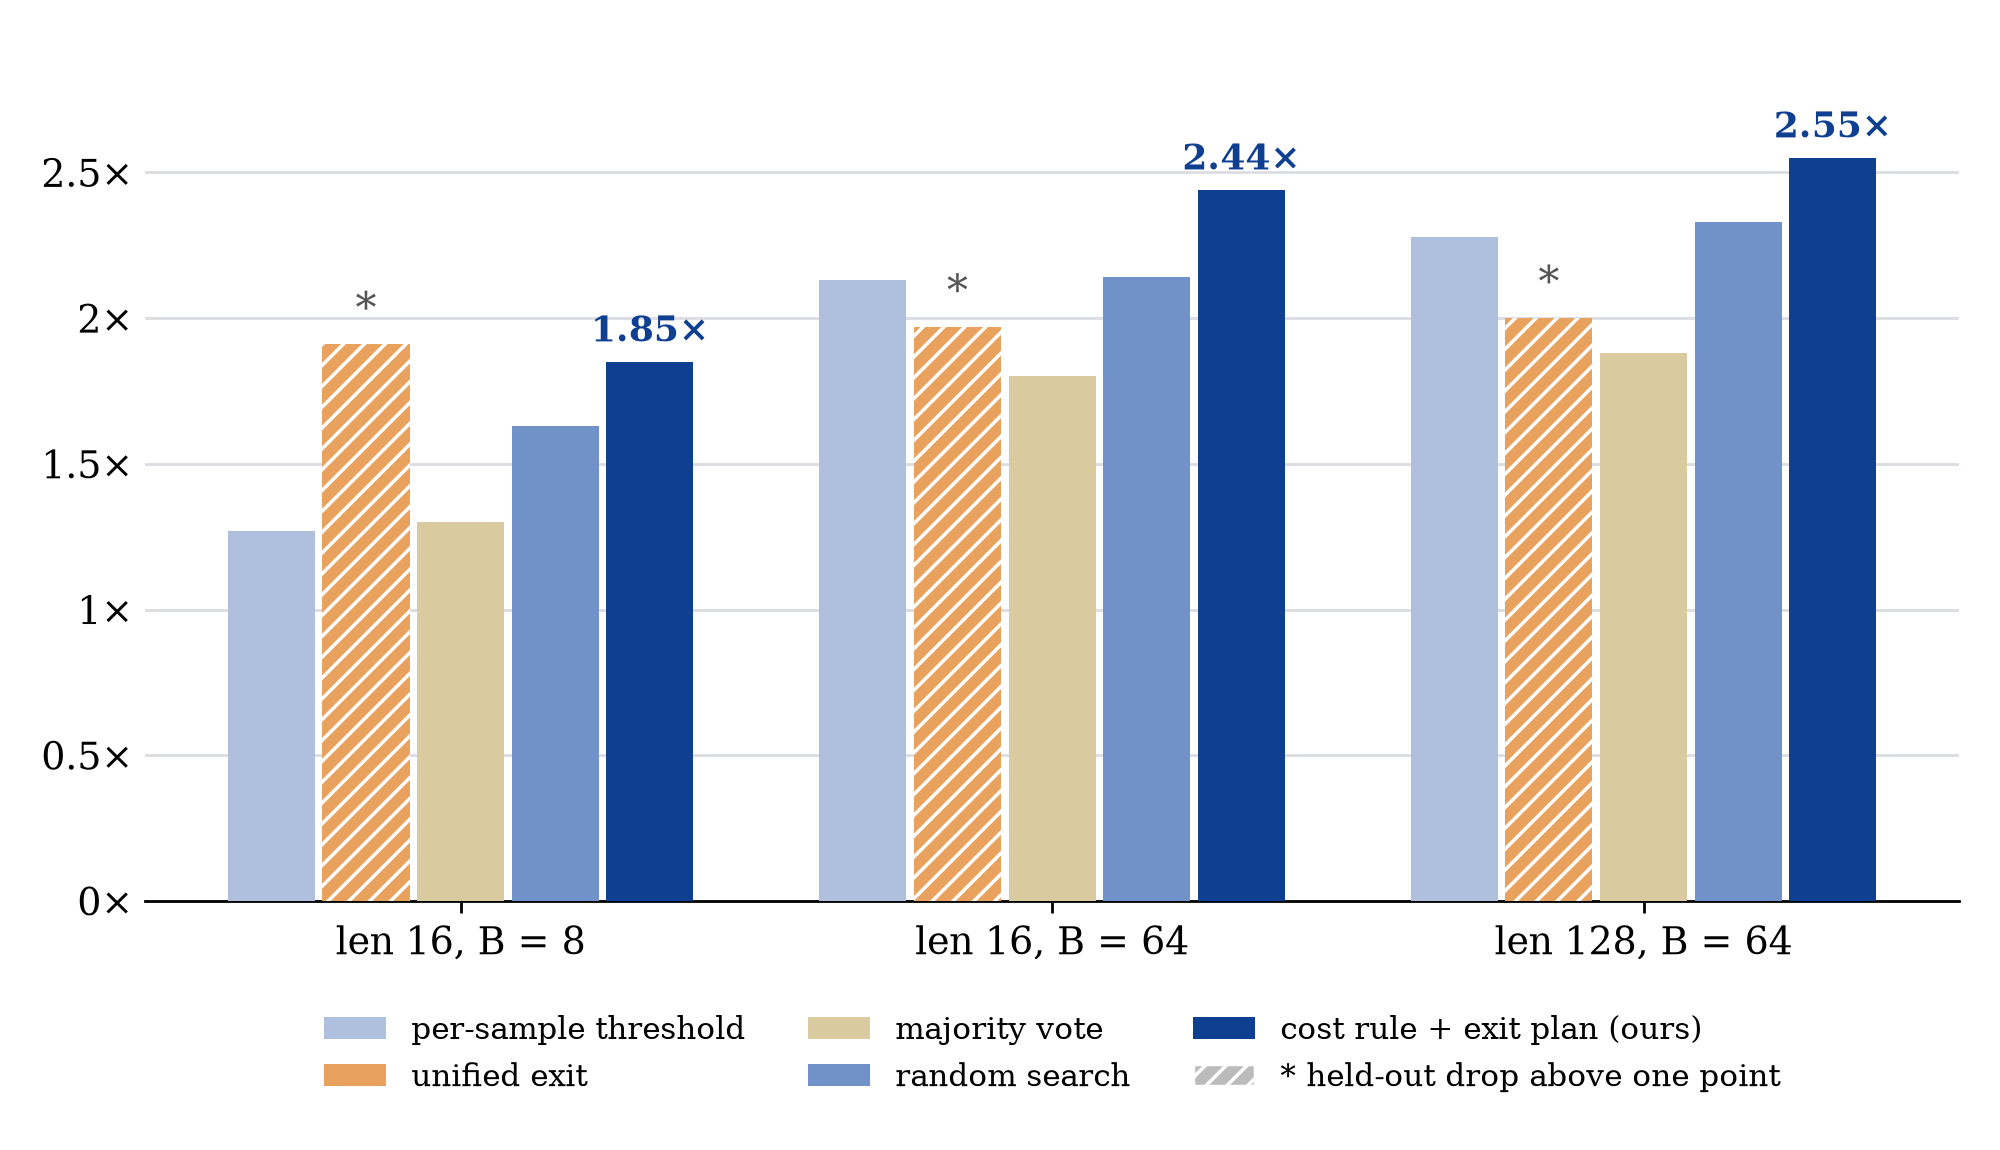
\includegraphics[width=0.78\textwidth]{fig/speedup.png}
  \caption{Speedup over the full model of each method's certified policy, QQP, GTX 1650, timed (values of
  Table~\ref{tab:t04}; chart of the final presentation, redrawn with the over-budget marks of the table).
  Hatched, $^{*}$: held-out drop above one point.}
  \label{fig:speedup}
\end{figure}

\begin{itemize}
  \item The fastest early-exit rule changes with batch size, execution mode and input length; a rule derived from the
  measured per-layer cost tracks it.
  \item At matched held-out accuracy it leads on QQP (2--17\% on the GTX 1650 cost table; 8--14\% timed on the A6000,
  replaying recorded decisions on a random-weight network) and on Llama classifiers with trained weights (3.66\x{}
  against 3.50\x). It has no gain on RoBERTa MNLI or on LLM decoders.
  \item Certified selection keeps the one-point budget on random re-splits (asymptotically); the finite-sample
  certificates are too loose to certify anything at our sample sizes.
  \item The bound on the damage from slowdown inputs is proved for the trimmed collective stop with a fixed active
  set; for the full rule it held empirically in all 25{,}200 batches tested (crafted inputs on CIFAR-100, the hardest
  natural inputs on MNLI and QQP). The label-free bandit has sublinear regret over ten seeds, with no rate claim.
  \item The accuracy loss of any batch-stopping rule lands on hard inputs (2.0--2.7 points on the hardest quarter of
  MNLI).
  \item \textbf{Lesson carried forward.} Search, by an LLM or otherwise, pays off where answers can be checked
  exactly. In early exit, LLM program search only tied our rule. That led us to index coding, where every bound is a
  certificate. The bridge was the Pincer agent (\file{pincer/}, results in \file{docs/PINCER.md}, Section~0, and
  \file{pincer/results/summary\_test2\_b30.md}): on a fresh split of 26 random-family graphs (30\,s per graph, 4-core
  container) its non-LLM policies closed the minrank gap on 13 of 26 graphs against 2 of 26 for the classic pipeline
  (CP-SAT~\cite{cpsat} independent set + TabuCol~\cite{tabucol} clique cover), and its data showed the Kneser pattern
  behind Part~II. An LLM in Pincer's loop did not beat these non-LLM policies.
\end{itemize}

% ---------------------------------------------------------------------------------------------------- 7
\section{Reproducing Part I step by step}\label{sec:repro1}

This section says what to do, in order, to obtain every number of Part~I from public data and models. Each step
gives the procedure and its parameters, the data it produces, and a check against the numbers reported above. The
file of the repository that implements each step is listed in Appendix~\ref{app:map}.

Two kinds of numbers appear. \emph{Measured} numbers (wall-clock speedups and the cost tables) need a GPU and will
differ slightly on other hardware. \emph{Replayed} numbers (selection, accuracy drops, fronts, re-splits,
certificates, load, bandit, robustness, theory) are computed on the CPU from the recorded traces and a cost table,
and are deterministic: given the same traces and cost tables they reproduce to the last printed digit. The traces
and cost tables we measured are committed, so every replayed number can be reproduced without a GPU by starting at
Step~R\ref{st:calib}.

\begin{figure}[ht]
  \centering
  \resizebox{\textwidth}{!}{%
  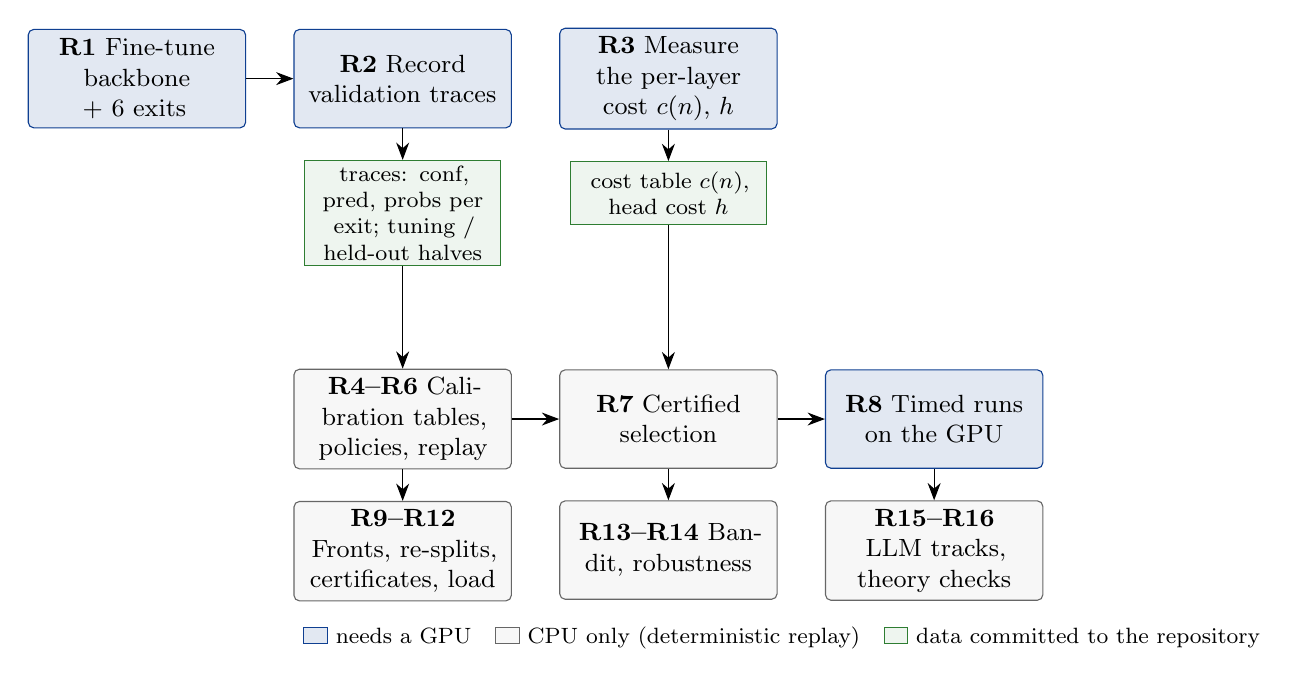
\begin{tikzpicture}[
      font=\small, >={Stealth[length=2.2mm]}, node distance=4mm and 6mm,
      gpu/.style={rectangle, rounded corners=2pt, draw=iitb, fill=iitb!12, align=center, text width=2.55cm,
                  minimum height=1.25cm, inner sep=3pt},
      cpu/.style={rectangle, rounded corners=2pt, draw=black!60, fill=black!3, align=center, text width=2.55cm,
                  minimum height=1.25cm, inner sep=3pt},
      dat/.style={rectangle, draw=okgreen, fill=okgreen!8, align=center, text width=2.35cm, minimum height=0.8cm,
                  font=\footnotesize, inner sep=2pt}]
    \node[gpu] (r1) {\textbf{R1} Fine-tune backbone + 6 exits};
    \node[gpu, right=of r1] (r2) {\textbf{R2} Record validation traces};
    \node[dat, below=of r2] (tr) {traces: conf, pred, probs per exit; tuning / held-out halves};
    \node[gpu, right=of r2] (r3) {\textbf{R3} Measure the per-layer cost $c(n)$, $h$};
    \node[dat, below=of r3] (ct) {cost table $c(n)$, head cost $h$};
    \node[cpu, below=13mm of tr] (r4) {\textbf{R4--R6} Calibration tables, policies, replay};
    \node[cpu, right=of r4] (r7) {\textbf{R7} Certified selection};
    \node[gpu, right=of r7] (r8) {\textbf{R8} Timed runs on the GPU};
    \node[cpu, below=of r4] (r9) {\textbf{R9--R12} Fronts, re-splits, certificates, load};
    \node[cpu, below=of r7] (r13) {\textbf{R13--R14} Bandit, robustness};
    \node[cpu, below=of r8] (r16) {\textbf{R15--R16} LLM tracks, theory checks};
    \draw[->] (r1) -- (r2);
    \draw[->] (r2) -- (tr);
    \draw[->] (r3) -- (ct);
    \draw[->] (tr) -- (r4);
    \draw[->] (ct) -- (r7);
    \draw[->] (r4) -- (r7);
    \draw[->] (r7) -- (r8);
    \draw[->] (r4) -- (r9);
    \draw[->] (r7) -- (r13);
    \draw[->] (r8) -- (r16);
    \node[anchor=north west, font=\footnotesize, align=left] at ($(r9.south west)+(0,-2mm)$)
      {\tikz\draw[draw=iitb,fill=iitb!12] (0,0) rectangle (0.3,0.2);~needs a GPU\quad
       \tikz\draw[draw=black!60,fill=black!3] (0,0) rectangle (0.3,0.2);~CPU only (deterministic replay)\quad
       \tikz\draw[draw=okgreen,fill=okgreen!8] (0,0) rectangle (0.3,0.2);~data committed to the repository};
  \end{tikzpicture}}
  \caption{The reproduction pipeline of Part~I. Every replayed result (grey) depends only on the committed traces and
  cost tables (green), so it can be reproduced on a CPU.}
  \label{fig:pipeline1}
\end{figure}

% ---------------------------------------------------------------------------------- R0
\subsection{Environment}
\begin{itemize}
  \item \textbf{Software.} Linux, Python 3.12.3, PyTorch 2.14.0 (CUDA 13.0), transformers 5.17.0, datasets 5.0.1,
  accelerate 1.15.0, numpy 2.5.3, scipy 1.18.1, pandas 3.0.6, scikit-learn 1.9.1 (isotonic regression), matplotlib
  3.11.2. Every package version we used is listed in Appendix~\ref{app:env}.
  \item \textbf{Hardware we used.} Server: 2\x{} Intel Xeon Silver 4216 (64 threads), 4\x{} RTX A6000 (48\,GB) and 2\x{} RTX 3080 Ti,
  NVIDIA driver 580.159.04; every server number in this report was measured on an RTX A6000. Laptop: GTX 1650 (4\,GB), 4 CPU threads. Any CUDA GPU can replace either; the measured
  speedups then change with it, the replayed numbers do not.
  \item \textbf{Data and models} (all public, from Hugging Face or torchvision): GLUE MNLI (\nolinkurl{validation_matched},
  9{,}815 examples) and QQP (\nolinkurl{validation}, 40{,}430) from \nolinkurl{nyu-mll/glue}; CIFAR-100 (test set, 10{,}000
  images) from torchvision; WikiText-103 (\nolinkurl{wikitext-103-raw-v1}) from \nolinkurl{Salesforce/wikitext}; backbones
  \nolinkurl{textattack/roberta-base-MNLI}, \nolinkurl{roberta-base}, \nolinkurl{google/vit-base-patch16-224-in21k},
  \nolinkurl{Qwen/Qwen2.5-1.5B}, \nolinkurl{meta-llama/Llama-3.1-8B-Instruct}, and the LayerSkip checkpoints
  \nolinkurl{facebook/layerskip-llama3.2-1B} and \nolinkurl{facebook/layerskip-llama3-8B}.
  \item \textbf{Conventions.} Speedup = full-model latency divided by the policy's latency at the same batch size.
  Drop = full-model accuracy minus policy accuracy, in points, on held-out data. Policies never see labels at decision
  time; labels are used only offline, to build calibration tables and to score.
\end{itemize}

% ---------------------------------------------------------------------------------- R1
\begin{step}{st:train}{Fine-tune each backbone jointly with its exits (GPU)}
\begin{enumerate}
  \item \textbf{Attach exits} after layers 2, 4, 6, 8, 10 and 12 of the 12-layer backbone; the exit after layer 12
  is the full model. A text exit is the RoBERTa classification head applied to the hidden state of the first token:
  dropout $\to$ Linear(768, 768) $\to$ tanh $\to$ dropout $\to$ Linear(768, classes). A ViT exit is LayerNorm
  $\to$ Linear(768, 100) on the class token.
  \item \textbf{Initialise.} MNLI: start from \texttt{textattack/roberta-base-MNLI} and copy its classifier into all
  six exit heads; its class order differs from GLUE's, so map checkpoint class $k$ to GLUE label $[2,1,0]_k$ (with
  the mapping the checkpoint scores 88.0\%, without it 28.5\%). QQP: start from \texttt{roberta-base} with randomly
  initialised heads. CIFAR-100: start from \texttt{google/vit-base-patch16-224-in21k}.
  \item \textbf{Loss.} The sum over exits of the cross-entropy of each exit, weighted by depth: the exit after layer
  $l$ has weight $l/\sum_{e} l_e$, i.e.\ $2/42, 4/42, \dots, 12/42$ (as in DeeBERT/PABEE).
  \item \textbf{Optimiser.} AdamW with two parameter groups (backbone and heads, each with its own learning rate),
  linear warm-up over the first warm-up fraction of steps followed by linear decay to zero, bf16 autocast, gradient
  norm clipped at 1.0. The training set is shuffled with seed 0. Text: premise and hypothesis (or the two questions)
  are tokenised as a pair, truncated to 128 tokens and padded to the longest sequence of the batch. Vision: images are
  resized from 32 to 224 pixels, augmented with pad-and-crop and horizontal flip, and normalised with mean = std = 0.5.
\end{enumerate}
\begin{center}\small
\begin{tabular}{@{}lccc@{}}
  \toprule
  Hyperparameter & MNLI & QQP & CIFAR-100 \\
  \midrule
  Initial weights & \makecell{\texttt{textattack/}\\\texttt{roberta-base-MNLI}} & \texttt{roberta-base} & \makecell{\texttt{google/vit-base-}\\\texttt{patch16-224-in21k}} \\
  Epochs / batch size & 2 / 64 & 2 / 64 & 4 / 128 \\
  Learning rate backbone / heads & $2\cdot10^{-5}$ / $2\cdot10^{-4}$ & $3\cdot10^{-5}$ / $2\cdot10^{-4}$ & $5\cdot10^{-5}$ / $10^{-3}$ \\
  Weight decay / warm-up fraction & 0.01 / 0.06 & 0.01 / 0.06 & 0.05 / 0.1 \\
  Dropout / label smoothing & 0.1 / 0 & 0.1 / 0 & 0 / 0.1 \\
  Max length / image size & 128 tokens & 128 tokens & 224 px \\
  Seed & 0 & 0 & 0 \\
  \bottomrule
\end{tabular}
\end{center}
\outp{a checkpoint per task (backbone + six heads) and a table of the accuracy of every exit.}
\chk{full-model (layer 12) validation accuracy 0.8777 (MNLI), 0.9106 (QQP), 0.9331 (CIFAR-100), Table~\ref{tab:models}.
One to three GPU-hours per model on an A6000.}
\end{step}

% ---------------------------------------------------------------------------------- R2
\begin{step}{st:traces}{Record the validation traces (GPU)}
\begin{enumerate}
  \item Run the whole validation set through the trained model once, in fp16 autocast, batch size 256, computing
  every exit (no early exit here).
  \item For every input $j$ and exit $e$ store the softmax vector $p_{j,e}$, the confidence
  $\text{conf}_{j,e}=\max_c p_{j,e,c}$ and the prediction $\text{pred}_{j,e}=\arg\max_c p_{j,e,c}$, plus the label.
  \item Split the validation set into two halves with a random permutation of seed 0: the first half of the
  permutation is the \emph{tuning} half (called ``evolve'' in the files), the rest is the \emph{held-out} half. All
  tuning, tables and selection use only the tuning half; every reported accuracy is on the held-out half.
\end{enumerate}
\outp{one trace table per task with columns \texttt{idx, label, split, conf\_e, pred\_e, p\_e\_c}.}
\chk{MNLI tuning half has about 4{,}900 inputs and QQP about 20{,}200. The traces we recorded are committed, so all
later CPU steps can start from them.}
\end{step}

% ---------------------------------------------------------------------------------- R3
\begin{step}{st:profile}{Measure the per-layer cost $c(n)$ and the head cost $h$ (GPU)}
\begin{enumerate}
  \item \textbf{Timing network.} Build the model of Step~R\ref{st:train} with random weights (\texttt{torch.manual\_seed(0)})
  in the dtype to be timed (fp32 on the GTX 1650). Timing does not depend on weight values. Make a pool of 512
  synthetic inputs of length $T\in\{16,32,128\}$: token ids uniform in $[5, 50000)$, first token 0, true length
  uniform in $[T/4, T]$ with the matching attention mask. (ViT: random $3\times224\times224$ images, 197 tokens.)
  \item \textbf{What one timed run does} (the same code path is used for the policies in Step~R\ref{st:time}): embed
  the batch; run the layers up to the next evaluated exit; apply that exit's head and softmax; copy the vector of
  maximum confidences to pinned host memory and synchronise (one host sync per evaluated exit); then continue.
  \item \textbf{Batch sizes} $B\in\{1,2,4,8,16,32,64,128\}$. For each $B$ time two plans: \emph{full} (only the last
  exit evaluated) and \emph{all heads} (all six exits evaluated, nobody leaves). Warm up once, then repeat each plan
  $r=\min(20,\max(3,\lfloor 20\,\text{s}/(0.02\,\text{s}\cdot B\,T/128)\rfloor))$ times and take the median; run
  the order full, heads, full, heads and average the two medians of each plan.
  \item \textbf{Derive} the per-layer cost $c(B) = t_{\text{full}}(B)/12$ and the head cost
  $h=\operatorname{median}_B\,(t_{\text{heads}}(B)-t_{\text{full}}(B))/5$. For reference fit the affine model
  $t_{\text{full}}(B)=12(a+bB)$ by least squares weighted by $1/t_{\text{full}}$ (relative error), and record
  $\rho=a/(bB)$ at $B=8$ and 64 and the largest relative error of the fit.
  \item \textbf{Cost table used by all later steps:} make $c(B)$ non-decreasing in $B$ with isotonic regression,
  interpolate linearly to every integer $n\in[0,256]$, extrapolate linearly beyond the last measured $B$, and set
  $c(0)=0$.
\end{enumerate}
\outp{one cost table per device, sequence length and model.}
\chk{Table~\ref{tab:cost} (GTX 1650): $c(1)\approx1.8$--2.3\,ms, $h\approx0.4$--0.5\,ms, affine error 41/31/10\% at
$T=16/32/128$; about 5 minutes per sequence length. The machine must be otherwise idle: the timed path synchronises
with the host after every exit, so CPU load from other jobs lowers the speedups and spreads them across rounds.}
\end{step}

% ---------------------------------------------------------------------------------- R4
\begin{step}{st:calib}{Build the calibration tables (CPU)}
For a set of tuning traces and an exit plan $S$ (the full plan has all six exits):
\begin{enumerate}
  \item For each evaluated exit $e$, cut its confidences into 20 bins at the quantiles of $\text{conf}_{\cdot,e}$
  (duplicate edges merged).
  \item In each bin $k$ and for every exit $e'$ of the plan estimate $P(\text{correct at } e' \mid \text{bin } k
  \text{ at } e)$ as $(\#\text{correct}+30\,\bar a_{e'})/(\#\text{inputs}+30)$, where $\bar a_{e'}$ is the overall
  accuracy of exit $e'$ (shrinkage with 30 pseudo-counts).
  \item Make each column non-decreasing in the bin index with isotonic regression weighted by the bin counts.
\end{enumerate}
The expected gain of input $j$ at exit $e$ is then $g_j(e\to e')=\max(0,\,P_{e'}(\text{bin}_j)-P_e(\text{bin}_j))$.
\end{step}

% ---------------------------------------------------------------------------------- R5
\begin{step}{st:policies}{Implement the policies and their candidate grids (CPU)}
Every policy is a function called at each evaluated exit (except the last) with the confidences of the $n$ active
inputs; it returns which inputs leave and whether the whole batch stops.
\begin{itemize}
  \item \textbf{Cost rule (ours).} With $F=12\,c(B)+h$, $\ell=L-l_e$ layers left and marginal cost
  $\Delta=c(n)-c(n-1)$ (for $n=1$ use $c(2)-c(1)$): input $j$ leaves if $g_j(e\to E)/B<\lambda\Delta\ell/F$, equation
  \eqref{eq:indiv}. If any inputs remain ($R$), the batch stops unless some later evaluated exit $e'$ has
  $\sum_{j\in R} g_j(e\to e')/B \ge \lambda[(l_{e'}-l_e)\,c(|R|)+(e'-e)\,h]/F$, equation~\eqref{eq:coll}.
  Grid: 40 values $\lambda\in\{10^{-3.5},\dots,10^{1.5}\}$, log-spaced.
  \item \textbf{Cost rule + exit plan.} Same rule on a plan $S$; the 31 plans are all non-empty subsets of the five
  intermediate exits, plus the last exit. Grid: every second $\lambda$ (20) \x{} 31 plans = 620 candidates. The
  calibration table is built on the plan's exits only.
  \item \textbf{Per-sample threshold:} input leaves if its confidence $>\tau$; 36 values $\tau\in[0.40,0.995]$ evenly
  spaced. \textbf{Threshold + exit plan:} every second $\tau$ (18) \x{} 31 plans = 558 candidates.
  \item \textbf{Majority vote:} the batch stops when more than half of the active inputs have confidence $>\tau$;
  same 36 values of $\tau$.
  \item \textbf{Unified exit:} every input leaves at one fixed intermediate exit (only that head is evaluated); 5
  candidates.
  \item \textbf{Random search:} a 3-parameter collective rule (per-sample threshold $\tau$; the batch also stops when
  the remaining share of the batch is below \texttt{frac\_cut} and their mean confidence exceeds \texttt{conf\_floor});
  150 candidates drawn with seed 0 from $\tau\sim U(0.5,1)$, $\texttt{frac\_cut}\sim U(0,0.5)$,
  $\texttt{conf\_floor}\sim U(0.3,0.95)$.
\end{itemize}
The counts above are for the six exits of the encoders. With $E$ exits the plans are the $2^{E-1}-1$ non-empty subsets
of the intermediate exits plus the last one; the LLM classifiers of Step~R\ref{st:llm} have $E=7$, so 63 plans, 1{,}260
candidates for the cost rule with a plan, 1{,}134 for the threshold with a plan and 6 unified exits.
\end{step}

% ---------------------------------------------------------------------------------- R6
\begin{step}{st:replay}{Replay a policy on recorded traces under a cost table (CPU)}
For each batch (a set of $B$ trace rows): walk through the evaluated exits of the plan in order; at each one add
(layers since the previous evaluated exit) \x{} $c(n)$ + $h$ to the batch's latency, where $n$ is the number of
active inputs, as in equation~\eqref{eq:latency}; at the last exit return the remaining predictions; otherwise call
the policy with the recorded confidences, return the recorded predictions of the inputs that leave and remove them.
The per-batch drop is the full model's accuracy on the batch minus the policy's; the speedup is $F$ divided by the
mean batch latency. This replay is exact for accuracy and is the ``cost-table'' speedup of Tables~\ref{tab:matched}
and~\ref{tab:resplit}.
\end{step}

% ---------------------------------------------------------------------------------- R7
\begin{step}{st:select}{Certified selection (CPU)}
For each task, batch size $B$ and method:
\begin{enumerate}
  \item Split the tuning half with a random permutation (seed 0) into a \emph{fit} part (40\%) and a \emph{cert}
  part (60\%). Cut each into disjoint random batches of size $B$ (permutation seeds $B$ and $B+1$).
  \item Build the calibration tables on the fit part. Replay every candidate on the fit batches.
  \item Order the candidates by mean drop (ascending), breaking ties by speedup (descending), and keep only those that
  are strictly faster than every candidate before them: this is the \emph{path} from safest to fastest.
  \item Walk along the path on the cert part. For each candidate compute the $K$ batch drops $Z_1,\dots,Z_K$, their
  mean $\bar Z$ and standard deviation $s$, and certify it if $(\alpha-\bar Z)/(s/\sqrt K) > t_{1-\delta,K-1}$ with
  $\alpha=0.01$ and $\delta=0.10$. Stop at the first candidate that is not certified.
  \item Return the fastest certified candidate (or none).
\end{enumerate}
The \emph{old protocol} of the first report, used for comparison in Table~\ref{tab:resplit}, pools fit and cert,
replays every candidate on it and takes the fastest one with empirical drop $\le\alpha$.
\outp{the certified parameters of every method at every $B$.}
\end{step}

% ---------------------------------------------------------------------------------- R8
\begin{step}{st:time}{Timed runs on the GPU}
\begin{enumerate}
  \item Take the held-out half and cut it into disjoint random batches of size $B$ (permutation seed $100+B$); time
  $n/B$ of them, with $n=1{,}920$ inputs at lengths 16 and 32 and $n=768$ at length 128 on the GTX 1650, and
  $n=2{,}048$ on the A6000. Each batch is mapped to $B$ random rows of the synthetic input pool (seed $B$).
  \item Policies timed: the full model, all heads with no exit (to measure the head overhead) and the certified
  policy of each method from Step~R\ref{st:select}, with calibration tables built on the fit part.
  \item Run one warm-up pass. Then, in each round, run every policy once over the same batches in a fixed order
  (interleaved), timing the whole pass with a host synchronisation before and after. The device executes exactly what
  Step~R\ref{st:profile} describes; after each host sync the confidences computed by the random-weight network are
  replaced by the trained model's recorded confidences for the same rows, the policy decides, and the leaving rows are
  removed from the hidden states with \texttt{index\_select}.
  \item Rounds: 5 at lengths 16 and 32 and 3 at length 128 (GTX 1650); 5 on the A6000. For each round compute the
  paired speedup (full time / policy time of the same round); report the median and the range over rounds.
  \item Confirm that the decisions taken on the device equal the replay of Step~R\ref{st:replay} for every batch,
  and compute the held-out drop by replaying the same policy on all held-out batches.
\end{enumerate}
\chk{Tables~\ref{tab:t04}--\ref{tab:t05} (GTX 1650, about 63 minutes in total) and
Tables~\ref{tab:t11}--\ref{tab:t12b} (A6000, about 28 minutes). Held-out drops must match exactly; speedups within a
few percent on the same GPU model, \emph{on an otherwise idle machine} (a loaded CPU spreads the rounds, because this
path synchronises after every exit).}
\end{step}

% ---------------------------------------------------------------------------------- R9
\begin{step}{st:front}{Accuracy--speed fronts and the hard quarter (CPU)}
\begin{enumerate}
  \item Run certified selection (Step~R\ref{st:select}) once per accuracy target
  $\alpha\in\{0.25, 0.5, 0.75, 1, 1.25, 1.5, 2, 3\}$ points, reusing one path per method and $B$.
  \item Score each selected policy once on the held-out half (disjoint batches, seed $100+B$) with the cost table:
  held-out drop and speedup. This gives Figure~\ref{fig:front}.
  \item Read each front at ``held-out drop $\le1$ point'': the fastest such point is the entry of
  Table~\ref{tab:matched}.
  \item Define the \emph{hard quarter} as the 25\% of held-out inputs with the lowest mean confidence over the five
  intermediate exits, and report the drop separately on it and on the rest at the one-point target
  (Table~\ref{tab:hard}, mean over $B=8,16,64$).
\end{enumerate}
\chk{Tables~\ref{tab:matched} and~\ref{tab:hard} exactly; about 5 minutes on 6 cores.}
\end{step}

% ---------------------------------------------------------------------------------- R10
\begin{step}{st:resplit}{Re-split validity check (CPU)}
Pool both halves of the traces. For each of 30 seeds $s$: permute with seed $1000+s$ and split into fit (20\%), cert
(30\%) and test (50\%); run certified selection (fit, cert) and the old protocol (fit + cert pooled); replay both
choices on disjoint test batches (seed $s+7$). Report the share of seeds whose test drop exceeds one point, the mean
drop and the mean speedup, at sequence length 16 with the GTX 1650 cost table, for $B=8$ and 64 and the three methods
of Table~\ref{tab:resplit}.
\chk{Table~\ref{tab:resplit} exactly (after the cache fix); about 8 minutes for both tasks on 6 cores. Build the
calibration table inside every re-split job from that job's fit part; never reuse a table across jobs
(Appendix~\ref{app:issues}).}
\end{step}

% ---------------------------------------------------------------------------------- R11
\begin{step}{st:certcheck}{Finite-sample and label-free certificates, and less calibration data (CPU)}
Repeat Step~R\ref{st:resplit} (30 seeds, 20/30/50\%) at $B=8,16,64,128$ with the A6000 cost table at length 128 (text)
and the A6000 ViT cost table (CIFAR-100), for five methods, with three certificates applied to the $K$ batch means of
the cert part: the $t$-test of Step~R\ref{st:select}; Hoeffding--Bentkus~\cite{rcps}; and the Waudby-Smith--Ramdas betting
bound~\cite{wsr}.
For the two finite-sample bounds map the batch drop from $[-1,1]$ to $[0,1]$. For the label-free version use the
disagreement with the full model's prediction as the risk (it upper-bounds the drop on every batch). For the data
experiment subsample both the fit and the cert parts to 10\%, 25\% and 50\%. Repeat MNLI with $\delta=5\%$.
\chk{Table~\ref{tab:cert}; about 1 h 47 min on 14 cores (3 h on 6 cores).}
\end{step}

% ---------------------------------------------------------------------------------- R12
\begin{step}{st:load}{Fluctuating load (CPU)}
\begin{enumerate}
  \item Generate an arrival trace: Poisson arrivals whose rate swings between light and heavy load (a sinusoid with a
  20\,s period plus bursts). A single server takes $\min(\text{queue},128)$ requests whenever it is free and serves a
  batch of size $B$ in the full model's time from the cost table. Record the sequence of batch sizes (3{,}000
  batches; 3 arrival seeds). All methods are replayed on the same sequence.
  \item For every method prepare three variants: certified once at $B=64$ (``once@64''), once at $B=8$
  (``once@8''), and re-certified per bucket $B\in\{1,2,4,\dots,128\}$ (each batch uses the parameters of the largest
  bucket $\le B$).
  \item Report the throughput speedup ($\sum$ full-model time / $\sum$ method time over all batches) and the drop over
  all served held-out inputs. Pass: tuned once, within budget, within 5\% of the best per-bucket baseline and ahead
  of every tuned-once baseline.
\end{enumerate}
\chk{Table~\ref{tab:load}; about 7 minutes per task.}
\end{step}

% ---------------------------------------------------------------------------------- R13
\begin{step}{st:bandit}{Label-free bandit (CPU)}
\begin{enumerate}
  \item Replace ``correct'' by ``agrees with the last exit'': keep, per exit $e$ and confidence bin $k$ (12 bins),
  the estimated rate $D[e,k,e']$ at which exit $e'$ disagrees with the last exit; the gain of going from $e$ to $e'$
  is $D[e,k,e]-D[e,k,e']$. No label is used.
  \item At batch $t$, with probability $\min(1, t^{-1/3})$ run a \emph{probe} batch to full depth (it still answers,
  at full cost) and update every table cell its inputs touch; otherwise run the cost rule with an optimistic
  (upper-confidence, $\beta=1$) gain, so that with little data it continues rather than stops. Use the $\lambda$ that
  the cost rule selected on the tuning half.
  \item Run $T=3{,}000$ batches of $B=64$ against an oracle that knows the true tables; record cumulative regret and
  fit its log--log slope. Use ten seeds (0--9) and three probe schedules: $\min(1,t^{-1/3})$, $\min(1,t^{-1/2})$, and a constant rate
  of 5\% of batches (probe probability $0.05\,t^{0}$); and a warm start
  from 20 labelled tuning batches. Baseline: a CeeBERT-style UCB1 over per-sample thresholds with reward = mean
  confidence $-$ $\mu\cdot$mean depth fraction.
\end{enumerate}
\chk{slopes 0.55--0.77 (Section~\ref{sec:bandit10}); about 22 minutes for ten seeds and six settings.}
\end{step}

% ---------------------------------------------------------------------------------- R14
\begin{step}{st:robust}{Slowdown inputs and the trimmed rule (CPU, plus one GPU step)}
\begin{enumerate}
  \item \textbf{Attack inputs.} ViT/CIFAR-100: a DeepSloth-style attack~\cite{sloth} (re-implemented): projected
  gradient descent in the $32\times32$ image space (before the resize to 224), $L_\infty$ budget $\varepsilon=8/255$,
  30 steps, loss $\sum_e \mathrm{CE}(\text{logits}_e,\text{uniform})$ so that no internal exit becomes confident, on
  500 images taken from the tuning half; record their traces as in Step~R\ref{st:traces} (GPU, once). Text tasks:
  use the hardest 2\% of held-out inputs as natural slowdown inputs.
  \item \textbf{Trimmed rule.} In the collective sum of~\eqref{eq:coll} drop the $m$ largest gains,
  $m\in\{0,B/16,B/8\}$.
  \item \textbf{Bound check.} For $k$ attackers, build 300 batches of $B=64$ with $B-k$ clean held-out inputs $C$ and
  $k$ attack inputs $K$; check $\operatorname{depth}(C\cup K;m)\le\operatorname{depth}(C;m-k)$ on every batch for
  every $k\le m$ (violations must be 0). Also record the victims' latency relative to the full model for
  $k\in\{0,1,2,4,8\}$ (16 and 32 in the final runs) and the same for majority vote, consensus and the threshold, all
  tuned by certified selection, on 4 cost profiles per task.
\end{enumerate}
\chk{0 violations in 25{,}200 batches; Section~\ref{sec:robust5}; about 7 minutes. The unit tests of the simulator and the bound
(19 tests) must pass.}
\end{step}

% ---------------------------------------------------------------------------------- R15
\begin{step}{st:llm}{LLM tracks (GPU for training and timing, CPU for the rest)}
\textbf{Batched classifiers} (Tables~\ref{tab:t15}--\ref{tab:t16}):
\begin{enumerate}
  \item Prompts. MNLI: \texttt{Premise: \{premise\}\textbackslash nHypothesis: \{hypothesis\}} followed by
  \texttt{\textbackslash nRelation of the hypothesis to the premise (entailment, neutral or contradiction):}. QQP:
  \texttt{Question 1: \{q1\}\textbackslash nQuestion 2: \{q2\}} followed by
  \texttt{\textbackslash nDo the two questions ask the same thing (yes or no)?}. Truncate to 128 tokens.
  \item Model. Freeze the base weights (bf16) and add LoRA~\cite{lora} (rank 16, $\alpha=32$) to the attention and MLP projections
  of every layer. Exits: Qwen2.5-1.5B after layers 4, 8, \dots, 28; Llama-3.1-8B after layers 8, 12, \dots, 32. Each
  exit is its own copy of the final norm followed by Linear($d$, classes), applied to the hidden state of the last
  prompt token.
  \item Train with the depth-weighted cross-entropy of Step~R\ref{st:train}: learning rate $2\cdot10^{-4}$ (LoRA)
  and $10^{-3}$ (heads); 8{,}000 steps at batch 16 for both models (128{,}000 training examples); seed 0. These are the values of the
  committed logs \file{logs/cls\_\{mnli,qqp\}\_\{qwen,llama\}.log}. The training script's defaults are 4{,}000
  steps at batch 32, and \file{scripts/reproduce\_gpu.sh} runs Qwen with those defaults, so pass
  \texttt{--steps 8000 --bs 16} for Qwen as well. Record traces as in
  Step~R\ref{st:traces}.
  \item Measure the cost table (Step~R\ref{st:profile}) and time the certified policies (Steps~R\ref{st:select},
  R\ref{st:time}) on the \emph{trained} weights with the real prompts padded to 128 tokens, in bf16. Check that the
  device's predictions agree with the traces (97--100\% at every exit).
\end{enumerate}
\textbf{Decoding} (Section~\ref{sec:llm}): train exit heads with LoRA (rank 16) or frozen (rank 0) on WikiText-103
next-token prediction (6{,}000 steps), record per-token traces, then, assuming a pure fixed cost ($b=0$), compare a
static exit (one exit for every batch, mixing adjacent exits at random to meet the budget exactly) with an adaptive
whole-batch stop (stop at the first exit where the batch's mean confidence reaches $\tau$), both tuned on the tuning
half to a one-point budget, for $B$ from 1 to 64.
\chk{Tables~\ref{tab:t15}--\ref{tab:t16}: Llama 60--63 minutes and Qwen 17--21 minutes of timing per task; adaptive
gain 12\% at $B=1$ falling to 0.2\% at $B=64$.}
\end{step}

% ---------------------------------------------------------------------------------- R16
\begin{step}{st:theory}{Theory checks (CPU)}
Enumerate small instances (a few inputs, 3--4 exits, monotone and non-monotone calibration tables, affine and floor
costs), compute the optimal policy by exact dynamic programming over (exit, active set), and compare it with
rules~\eqref{eq:indiv} and~\eqref{eq:coll}. Then replay the corrected per-input rule (test every later exit) against
the implemented one on the real traces (QQP, MNLI; both cost tables; $B=8$--128) and compare them at the certified
one-point target and at matched held-out drop.
\chk{210/210 and 17/190 (collective), 301 and 165 (per-input), 40 real-trace settings with $-1.4\%$ at matched drop
(Section~\ref{sec:theory}); about 10 seconds for the exact checks and 20 minutes for the real traces.}
\end{step}

\subsection{Checking a reproduction}
\begin{itemize}
  \item Every number printed in Part~I can be recomputed from the result files and compared with the text; we did
  this for every table cell (all match) and every number in the text (the ten that do not match the committed files are corrected and marked
  above).
  \item We regenerated every CPU-derived result file from the committed traces and cost tables on 25 November (72
  steps, 5\,h\,16\,min on 6 cores, CPU only): 92 of 102 files matched to the last printed digit. The other 10 differed
  only in cost-rule rows because of the cache bug of Appendix~\ref{app:issues}; after the fix, runs with 3 and 6
  workers give identical files.
  \item GPU numbers cannot be checked without a GPU; their raw logs are committed next to the result files.
\end{itemize}

% ==================================================================================================== PART II
\part{Kneser graphs: exact minrank and an agent that proves it}
\label{part:kneser}

% ---------------------------------------------------------------------------------------------------- 8
\section{Exact minrank of Kneser graphs}\label{sec:minrank}

\subsection{Index coding, minrank and Kneser graphs}
\textbf{Index coding~\cite{baryossef}.} A sender holds one message per receiver. Receiver $v$ wants its own message
and already knows the messages of its neighbours in a graph $G$. How few broadcasts suffice? For every field $F$,
\begin{equation}
  \underbrace{\alpha(G)}_{\text{lower bound}} \;\le\; \underbrace{\beta(G)}_{\text{optimum}} \;\le\;
  \underbrace{\operatorname{minrk}_F(G)}_{\text{best linear code}} \;\le\; \underbrace{\bar\chi(G)}_{\text{clique cover}}.
\end{equation}
Here $\alpha$ is the independence number (the most receivers with no side information about each other), $\beta$
the broadcast rate, $\operatorname{minrk}_F$ the minrank over $F$ (the least rank of a matrix that \emph{fits} $G$:
nonzero diagonal, zero on non-adjacent pairs), and $\bar\chi$ the clique cover number. The best scalar linear code
over $F$ has length $\operatorname{minrk}_F(G)$~\cite{baryossef}. Exact $\beta$ is known for very few graph families.

\begin{figure}[ht]
  \centering
  \begin{minipage}{0.36\textwidth}\centering
    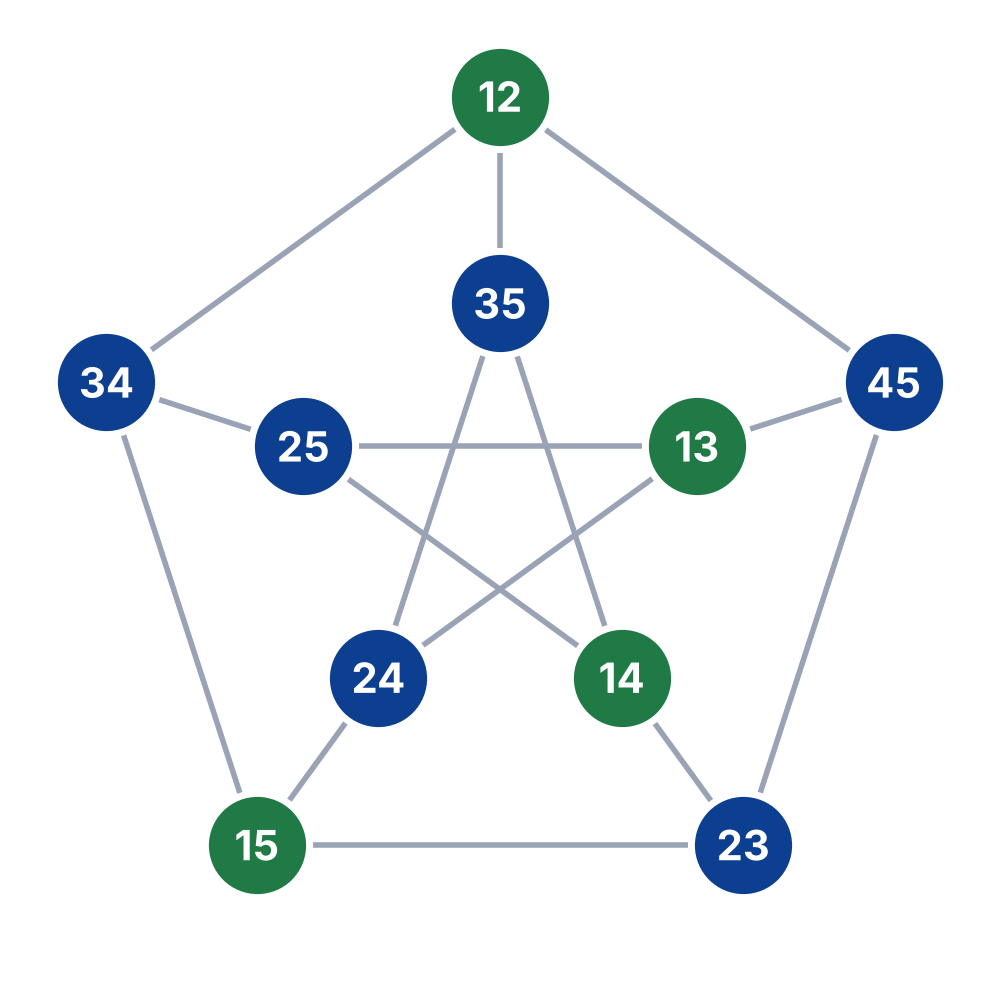
\includegraphics[width=\linewidth]{fig/k52.png}
  \end{minipage}\hfill
  \begin{minipage}{0.58\textwidth}
    \caption{The Kneser graph $K(5,2)$: 10 receivers (the pairs from $\{1,\dots,5\}$), two adjacent iff disjoint.
    Green: the 4 pairs containing 1. No two of them are adjacent, so $\alpha=4$: the Erd\H{o}s--Ko--Rado star.}
    \label{fig:k52}
  \end{minipage}
\end{figure}

\textbf{Kneser graph $K(n,k)$.} Receivers are all $k$-element subsets of $\{1,\dots,n\}$; two are adjacent iff
disjoint. By the Erd\H{o}s--Ko--Rado theorem~\cite{ekr}, $\alpha=\binom{n-1}{k-1}$, attained by the star $S=\{A: 1\in A\}$
(Figure~\ref{fig:k52}).

\subsection{The theorem}
Let $D$ be the disjointness (adjacency) matrix of $K(n,k)$, $\varepsilon=(-1)^{k-1}$ and $H=I+\varepsilon D$;
equivalently $H_{A,B}=\binom{|A\cap B|-1}{k-1}$. $H$ fits $K(n,k)$ over every field (it is the matrix of
Golovnev--Haviv~\cite{gh}, who bounded its rank by $\sum_{i<k}\binom{n}{i}$). For a prime $p$ let $q=q_p(k)$ be the
least power of $p$ with $q\ge k$.

\begin{theorem}\label{thm:rank}
For every prime $p$ and $n>2k\ge4$:
\[
  \operatorname{rank}_{\Fp}(I+\varepsilon D) = \binom{n-1}{k-1} \iff q_p(k) \mid n-2k .
\]
In particular, if $q\mid n-2k$ then $\operatorname{minrk}_{\Fp}(K(n,k))=\beta=\alpha$.
\end{theorem}

\begin{theorem}[explicit optimal index code]\label{thm:code}
If $q_p(k)\mid n-2k$, the following scalar linear code over $\Fp$ uses $\alpha=\binom{n-1}{k-1}$ transmissions,
optimal among all (also non-linear) index codes. For every $k$-set $A$ containing 1, broadcast
\[
  y_A = x_A + \varepsilon \sum_{B\cap A=\emptyset} x_B .
\]
A receiver $A\ni1$ decodes $x_A$ from $y_A$ (it knows every $x_B$ with $B$ disjoint from $A$). A receiver $A'\not\ni1$
computes $\varepsilon\sum_{A\ni1,\,A\cap A'=\emptyset} y_A = x_{A'}+\varepsilon\sum_{B\cap A'=\emptyset}x_B$ and
subtracts its side information.
\end{theorem}

\begin{corollary}[broadcast rate]
For every $k\ge2$ and all but finitely many $n$, $\beta(K(n,k))=\binom{n-1}{k-1}$, attained by a scalar linear code
over a suitable prime field. The field cannot be fixed in advance:
$\operatorname{minrk}_{\mathbb{F}_2}(K(7,2))=7>6=\operatorname{minrk}_{\mathbb{F}_3}(K(7,2))$.
\end{corollary}

\subsection{Proof}
Write $m=n-2k\ge1$.
\begin{enumerate}
  \item \textbf{Star rows are independent.} $H$ restricted to $S\times S$ is the identity (two members of $S$ share
  the element 1), so $\operatorname{rank}H\ge\alpha$ over every field.
  \item \textbf{Decoding identity.} For $A'\notin S$ and any $k$-set $B$, let
  $R(A',B)=\sum_{A\in S,\,A\cap A'=\emptyset}H_{A,B}$. If $1\in B$ then $\varepsilon R=H_{A',B}$. If $1\notin B$ then
  $\varepsilon R=\binom{m-1+t}{k-1}$ with $t=|A'\cap B|$, while $H_{A',B}=\binom{t-1}{k-1}$.
  \item \textbf{Rank $\alpha$ iff a congruence.} $\operatorname{rank}_p H=\alpha$ iff
  $\binom{m-1+t}{k-1}\equiv\binom{t-1}{k-1}\pmod p$ for $t=0,1,\dots,k$. ($\Leftarrow$: every row outside $S$ is
  $\varepsilon$ times the sum of the disjoint star rows. $\Rightarrow$: restricting to the star columns, where $H=I$,
  forces those coefficients, and every $t$ occurs.)
  \item \textbf{Lucas' theorem~\cite{lucas}.} With $g(x)=\binom{x+m}{k-1}-\binom{x}{k-1}=\sum_{i=1}^{k-1}\binom{m}{i}\binom{x}{k-1-i}$
  (Vandermonde), the congruences are equivalent to $\binom{m}{i}\equiv0\pmod p$ for $1\le i\le k-1$, which by Lucas'
  theorem holds iff $q_p(k)\mid m$.
\end{enumerate}
Since $H$ fits $K(n,k)$, $\operatorname{minrk}_{\Fp}\le\alpha$ in those cases; $\alpha$ is a lower bound for every
index code, so the linear code is optimal. \qed

A second, independent proof of the ``if'' direction via the integer diagonal forms of Ducey et al.~\cite{ducey},
and a third for $k=3$ via inclusion matrices, are in \file{proof.md} of the repository.

\subsection{Which cases are new}
Known before: for $k\mid n$, Baranyai's theorem~\cite{baranyai} partitions the $k$-sets into $\binom{n-1}{k-1}$ perfect matchings
(cliques), so $\operatorname{minrk}=\alpha$ over every field. \textbf{New:} the exact $p$-rank of $H$ with an
if-and-only-if condition, the explicit code and decoder, and infinitely many $n$ with $k\nmid n$ for every $k$, where
even the fractional clique cover exceeds $\alpha$. Construction: take a prime $p>k$ and $n=2k+pt$ with
$t\equiv1\pmod k$. \textbf{Not claimed:} anything about other fields, or $\operatorname{minrk}>\alpha$ when
$q\nmid n-2k$ (then this $H$ has rank above $\alpha$, nothing more). The theorem gives $\operatorname{minrk}=\alpha$ only in the
\emph{if} direction: when $q\nmid n-2k$, $\operatorname{minrk}$ can still equal $\alpha$ through another matrix. For
example $K(9,3)$ over $\mathbb{F}_2$: $q_2(3)=4$ does not divide $3$, yet $3\mid9$, so Baranyai's theorem gives
$\operatorname{minrk}_{\mathbb{F}_2}=\alpha$.

\textbf{Relation to Ducey et al.~\cite{ducey}.} Their integer diagonal forms of the subset-intersection matrices
$D-\lambda I$ (for $n\ge3k-1$) reduce $\operatorname{rank}_pH$ to a weighted sum of the ranks of $k+1$ small
integer matrices, and our second proof (\file{proof.md}, Appendix~A) starts from that reduction. Their paper does
not evaluate these ranks for $H$ or state when the sum equals $\alpha$. What is new here beyond it is: the closed
form, $\operatorname{rank}_pH=\alpha$ if and only if $q_p(k)\mid n-2k$, for every $n>2k$ (a proof from their forms gives only
the ``if'' direction); the elementary proof above, which does not use diagonal forms; and
the consequences for index coding, namely $\operatorname{minrk}=\beta=\alpha$, the explicit code and decoder, and the
cases with $k\nmid n$. Our search of the literature (\file{proof.md}, Remark~5.5) found no exact minrank or
broadcast-rate values for Kneser graphs beyond the $k\mid n$ case; it was a web search, not an exhaustive review.

\begin{table}[ht]
  \centering\small
  \begin{minipage}[t]{0.52\textwidth}\centering
    \begin{tabular}{@{}llrr@{}}
      \toprule
      Graph & Field & $\operatorname{minrk}=\alpha$ & Fractional cover \\
      \midrule
      $K(7,2)$  & $\mathbb{F}_3$ & 6   & 7 \\
      $K(10,3)$ & $\mathbb{F}_2$ & 36  & 40 \\
      $K(13,4)$ & $\mathbb{F}_5$ & 220 & 238.3 \\
      $K(15,4)$ & $\mathbb{F}_7$ & 364 & 455 \\
      \bottomrule
    \end{tabular}\par\smallskip
    (a) New cases with $k\nmid n$: no clique cover reaches $\alpha$.
  \end{minipage}\hfill
  \begin{minipage}[t]{0.44\textwidth}\centering
    \begin{tabular}{@{}cl@{}}
      \toprule
      $k$ & \makecell{$n$ with $k\nmid n$ covered\\by no prime} \\
      \midrule
      2 & 5 \\
      3 & 7, 8 \\
      4 & 9, 10, 11, 14 \\
      5 & 11, 12, 13, 14, 16, 22 \\
      6 & 13, 14, 15, 16, 17, 22, 27, 32 \\
      \bottomrule
    \end{tabular}\par\smallskip
    (b) The finitely many exceptions. Values with $k\mid n$\\ (e.g.\ 18, 24, 42, 72 for $k=6$) are left\\ out: Baranyai's theorem covers them.
  \end{minipage}
  \caption{Which cases the theorem settles.}
  \label{tab:newcases}
\end{table}

\subsection{Worked example: an optimal code for $K(7,2)$ over $\mathbb{F}_3$}
$K(7,2)$ has 21 receivers (pairs from $1..7$); $q_3(2)=3$ divides $7-4$, so Theorem~\ref{thm:rank} applies with
$\varepsilon=-1$. For each pair $A=\{1,j\}$ broadcast $y_A=x_A-\sum_{B\cap A=\emptyset}x_B\pmod3$: 6 broadcasts $=\alpha$,
against 7 for the clique-cover code and 7 for the best linear code over $\mathbb{F}_2$. Receiver $\{1,4\}$ knows every
$x_B$ with $B$ disjoint from it, so it reads $x_{14}$ from $y_{14}$. Receiver $\{2,3\}$ computes
$-(y_{14}+y_{15}+y_{16}+y_{17})=x_{23}-\sum_{B\cap\{2,3\}=\emptyset}x_B$ and removes the sum it knows. Checked
numerically on random messages. Over $\mathbb{F}_2$ no 6-broadcast linear code exists (SAT, DRAT-checked).

\subsection{Evidence and computer proofs}
\begin{itemize}
  \item 318 $(n,k,p)$ cases with $\binom nk\le2000$: the row identity $\iff\operatorname{rank}_pH=\alpha\iff q\mid
  n-2k$; the congruence of step 4 checked for $k\le12$, $p\le13$, $m=n-2k\le400$.
  \item 82 cases checked by two independent rank codes (FLINT and an own Gaussian elimination mod $p$),
  $\binom nk\le3500$, $k\le6$; 39 of them with $k\nmid n$.
  \item 6{,}666 cases of the second proof (integer diagonal forms) agree with Theorem~\ref{thm:rank} ($k\le12$,
  $n\le120$, $p\le13$).
  \item $K(7,2)$ over $\mathbb{F}_2$: rank $\le6$ refuted by SAT; the UNSAT proof checked by drat-trim (0.39\,s).
  \item $\operatorname{minrk}_{\mathbb{F}_2}(K(7,3))=18$ and $\operatorname{minrk}_{\mathbb{F}_2}(K(8,3))=22$, above
  $\alpha=15$ and 21 (DRAT-checked; $K(8,3)$ at rank 21: solve 950\,s, check 1{,}663\,s).
  \item Open: $K(9,2)$ and $K(11,2)$ over $\mathbb{F}_2$; a star-basis SAT reduction (0.3\,s on $K(7,2)$, over 1\,h
  before) did not finish in 2\,h.
\end{itemize}

% ---------------------------------------------------------------------------------------------------- 9
\section{The Kneser agent: an LLM agent that proves the broadcast rate}\label{sec:agent}

\subsection{Why an agent?}
\begin{itemize}
  \item \textbf{Proving $\beta$ gets slow.} Standard methods (the CP-SAT constraint solver~\cite{cpsat} for $\alpha$ and
  the clique cover, the fractional cover, and $\mathbb{F}_2$ minrank by SAT) prove 2 of 25 benchmark graphs in 60\,s each. One
  certified rank check costs about $N^2r$: on $N=14{,}950$ receivers, 54\,s.
  \item \textbf{Real inputs arrive unlabelled:} vertices shuffled, no family name. The theorem helps only if someone
  recognises the structure and picks the right field and constant.
  \item \textbf{Idea.} An LLM reads a numeric summary of the graph, guesses its structure and plans which certified
  checks to run. A pool of worker processes runs the checks; the run stops the moment lower bound $=$ upper bound.
  Only certified results count, and an independent verifier re-checks the final code. The LLM never writes a bound.
\end{itemize}

\textbf{Baseline: the Kneser agent without an LLM} (Kushagra's script, Figure~\ref{fig:baseline}). A fixed sequence:
recognise $(n,k)$ from the vertex count and degree; the theorem names the prime; one exact rank (FLINT~\cite{flint})
gives the code length; a greedy independent set gives the lower bound; anything that does not certify goes to a
general minrank solver, so a wrong guess can never produce a wrong answer. The greedy step runs only on a recognised
Kneser graph: on any other graph the script goes straight to the general solver and reports that solver's bounds.

\begin{figure}[ht]
  \centering
  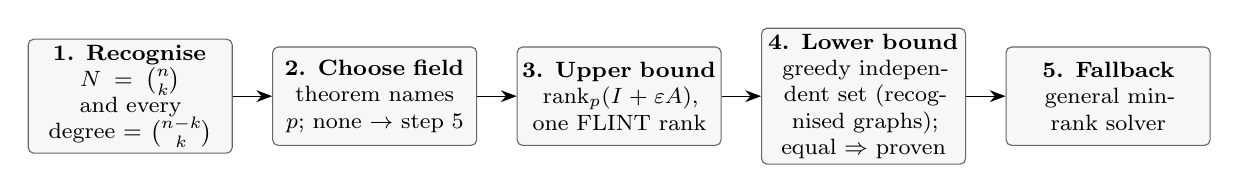
\begin{tikzpicture}[font=\footnotesize, >={Stealth[length=2mm]}, node distance=5mm,
      s/.style={rectangle, rounded corners=2pt, draw=black!60, fill=black!3, align=center, text width=2.45cm,
                minimum height=1.25cm, inner sep=2pt}]
    \node[s] (a) {\textbf{1. Recognise}\\$N=\binom nk$ and every degree $=\binom{n-k}{k}$};
    \node[s, right=of a] (b) {\textbf{2. Choose field}\\theorem names $p$; none $\to$ step 5};
    \node[s, right=of b] (c) {\textbf{3. Upper bound}\\$\operatorname{rank}_p(I+\varepsilon A)$, one FLINT rank};
    \node[s, right=of c] (d) {\textbf{4. Lower bound}\\greedy independent set (recognised graphs); equal $\Rightarrow$ proven};
    \node[s, right=of d] (e) {\textbf{5. Fallback}\\general minrank solver};
    \draw[->] (a) -- (b); \draw[->] (b) -- (c); \draw[->] (c) -- (d); \draw[->] (d) -- (e);
  \end{tikzpicture}
  \caption{The baseline Kneser agent (no LLM): five fixed steps, full exact rank ($O(N^3)$).}
  \label{fig:baseline}
\end{figure}

\subsection{Architecture of our agent}\label{sec:arch}

Figure~\ref{fig:arch} shows the architecture. Two kinds of component alternate: LLM roles (dark) that only decide
\emph{what to check}, and code (light) that computes and certifies every number. The verdict comes from the checks,
not from an LLM.

\begin{figure}[p]
  \centering
  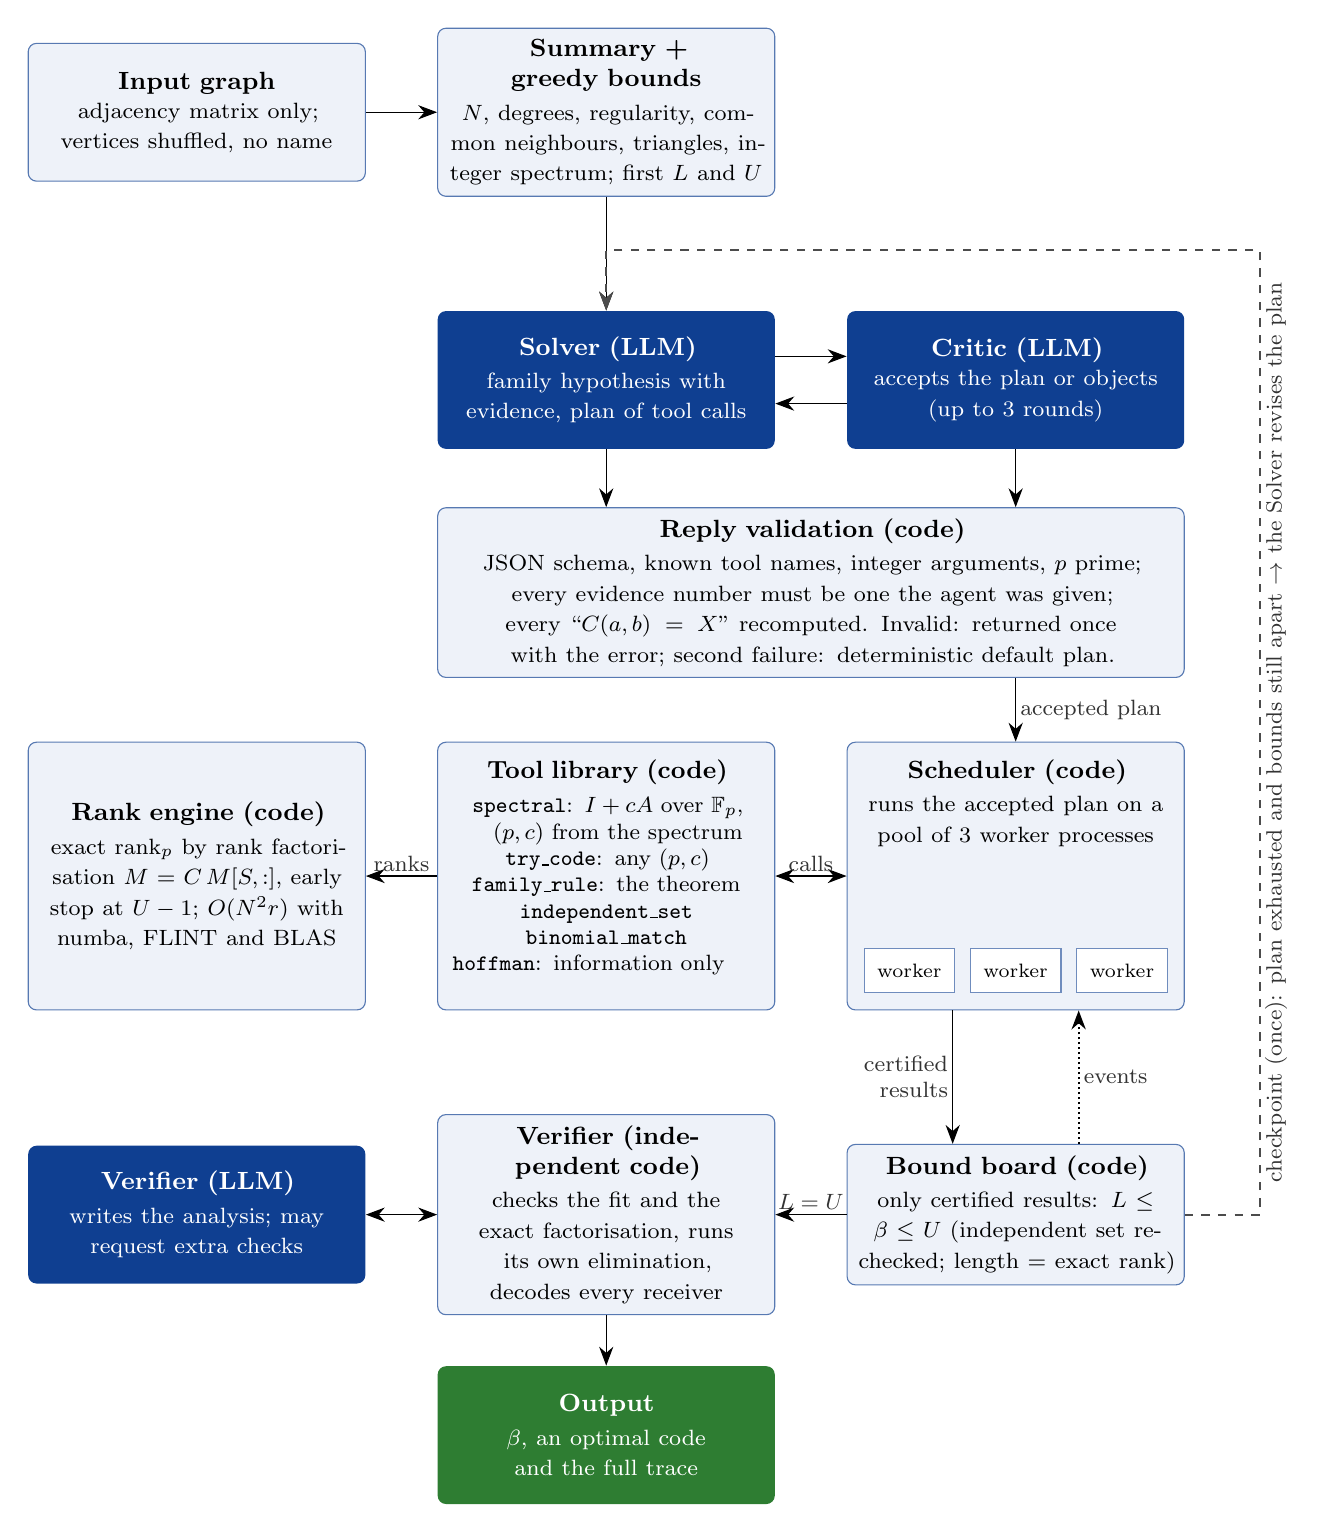
\begin{tikzpicture}[
      font=\small, >={Stealth[length=2.4mm]},
      box/.style={rectangle, rounded corners=3pt, align=center, text width=4.0cm, minimum height=1.75cm, inner sep=4pt},
      llmb/.style={box, fill=llm, text=white},
      code/.style={box, draw=iitb!70, fill=codebox},
      resbox/.style={box, fill=okgreen, text=white},
      d/.style={font=\footnotesize},
      lab/.style={font=\footnotesize, align=center, text=black!80, inner sep=1.5pt}]
    % row A
    \node[code] (g) at (0,0) {\textbf{Input graph}\\[1pt]{\footnotesize adjacency matrix only;\\vertices shuffled, no name}};
    \node[code] (s) at (5.2,0) {\textbf{Summary + greedy bounds}\\[1pt]{\footnotesize $N$, degrees, regularity,
      common neighbours, triangles, integer spectrum; first $L$ and $U$}};
    % row B
    \node[llmb] (so) at (5.2,-3.4) {\textbf{Solver (LLM)}\\[1pt]{\footnotesize family hypothesis with evidence,
      plan of tool calls}};
    \node[llmb] (cr) at (10.4,-3.4) {\textbf{Critic (LLM)}\\[1pt]{\footnotesize accepts the plan or objects\\(up to 3 rounds)}};
    % row C
    \node[code, text width=9.2cm, minimum height=1.5cm] (val) at (7.8,-6.1) {\textbf{Reply validation (code)}\\[1pt]
      {\footnotesize JSON schema, known tool names, integer arguments, $p$ prime; every evidence number must be one the
      agent was given; every ``$C(a,b)=X$'' recomputed. Invalid: returned once with the error; second failure:
      deterministic default plan.}};
    % row D
    \node[code, minimum height=3.4cm] (rk) at (0,-9.7) {\textbf{Rank engine (code)}\\[1pt]{\footnotesize exact
      $\operatorname{rank}_p$ by rank factorisation $M=C\,M[S,:]$, early stop at $U-1$; $O(N^2r)$ with numba, FLINT and
      BLAS}};
    \node[code, minimum height=3.4cm] (tl) at (5.2,-9.7) {};
    \node[anchor=north, text width=3.9cm, align=left, font=\footnotesize] at ([yshift=-3pt]tl.north)
      {\centering\textbf{\small Tool library (code)}\par\smallskip
       \texttt{spectral}: $I+cA$ over $\Fp$,\\ \quad$(p,c)$ from the spectrum\\
       \texttt{try\_code}: any $(p,c)$\\
       \texttt{family\_rule}: the theorem\\
       \texttt{independent\_set}\\
       \texttt{binomial\_match}\\
       \texttt{hoffman}: information only};
    \node[code, minimum height=3.4cm] (sch) at (10.4,-9.7) {};
    \node[anchor=north, text width=3.9cm, align=center] at ([yshift=-3pt]sch.north)
      {\textbf{Scheduler (code)}\\[1pt]{\footnotesize runs the accepted plan on a pool of 3 worker processes}};
    \foreach \i/\xx in {1/9.05, 2/10.4, 3/11.75}
      \node[rectangle, draw=iitb!60, fill=white, minimum width=1.15cm, minimum height=0.55cm, font=\scriptsize]
        at (\xx,-10.9) {worker};
    % row E
    \node[llmb] (vl) at (0,-14.0) {\textbf{Verifier (LLM)}\\[1pt]{\footnotesize writes the analysis; may request
      extra checks}};
    \node[code] (ve) at (5.2,-14.0) {\textbf{Verifier (independent code)}\\[1pt]{\footnotesize checks the fit and the exact factorisation, runs its own elimination, decodes every receiver}};
    \node[code] (bd) at (10.4,-14.0) {\textbf{Bound board (code)}\\[1pt]{\footnotesize only certified results:
      $L\le\beta\le U$ (independent set re-checked; length = exact rank)}};
    % row F
    \node[resbox] (o) at (5.2,-16.8) {\textbf{Output}\\[1pt]{\footnotesize $\beta$, an optimal code and the full trace}};
    % arrows
    \draw[->] (g) -- (s);
    \draw[->] (s) -- (so);
    \draw[->] ([yshift=3mm]so.east) -- ([yshift=3mm]cr.west);
    \draw[->] ([yshift=-3mm]cr.west) -- ([yshift=-3mm]so.east);
    \draw[->] (so.south) -- (so.south |- val.north);
    \draw[->] (cr.south) -- (cr.south |- val.north);
    \draw[->] (val.south -| sch.north) -- node[lab, right] {accepted plan} (sch.north);
    \draw[<->] (tl.east) -- node[lab, above] {calls} (sch.west);
    \draw[->] (tl.west) -- node[lab, above] {ranks} (rk.east);
    \draw[->] ([xshift=-8mm]sch.south) -- node[lab, left, text width=1.7cm, align=right] {certified results}
      ([xshift=-8mm]bd.north);
    \draw[->, densely dotted, thick] ([xshift=8mm]bd.north) -- node[lab, right] {events} ([xshift=8mm]sch.south);
    \draw[->] (bd.west) -- node[lab, above] {$L=U$} (ve.east);
    \draw[<->] (ve.west) -- (vl.east);
    \draw[->] (ve.south) -- (o.north);
    \draw[->, dashed, thick, black!70] (bd.east) -- (13.5,-14.0) -- node[lab, rotate=90, below, pos=0.5]
      {checkpoint (once): plan exhausted and bounds still apart $\to$ the Solver revises the plan}
      (13.5,-1.75) -- (5.2,-1.75) -- (so.north);
  \end{tikzpicture}
  \par\medskip
  {\footnotesize
   \tikz\fill[llm] (0,0) rectangle (0.35,0.22);~LLM role \qquad
   \tikz{\fill[codebox] (0,0) rectangle (0.35,0.22); \draw[iitb!70] (0,0) rectangle (0.35,0.22);}~code \qquad
   \tikz\fill[okgreen] (0,0) rectangle (0.35,0.22);~result \qquad
   dashed: checkpoint loop\\[2pt] dotted: scheduler events (new bound $\to$ retarget; near miss $\to$ more constants for that field; $L=U$ $\to$ stop)}
  \caption{Architecture of the Kneser agent. The LLMs (Solver, Critic, Verifier) only decide what to check and explain
  the result; every number on the bound board is a certificate computed by code, and the final verdict comes from
  independent checking code that shares nothing with the tools. If the LLM's plans leave the bracket open after the
  checkpoint, a deterministic generic search still runs (safety net). The LLM is called only at the start, at the
  checkpoint and at the end.}
  \label{fig:arch}
\end{figure}

\textbf{Components.}
\begin{enumerate}
  \item \textbf{Input.} Only the adjacency matrix; the benchmark relabels the vertices with a random permutation
  (\texttt{--seed}) and never passes the graph's name.
  \item \textbf{Summary and greedy bounds (code).} Number of receivers, degree sequence, regularity, sampled
  common-neighbour counts, triangle count, and the integer spectrum with multiplicities. A greedy independent set and
  a greedy cover give the first bracket $[L,U]$ before any LLM call.
  \item \textbf{Solver and Critic (LLMs).} The Solver reads the summary and writes a family hypothesis with evidence
  (numbers from the summary) and a plan of tool calls; the Critic accepts it or objects, for up to 3 rounds. The
  system prompts are in Appendix~\ref{app:prompts}.
  \item \textbf{Reply validation (code).} Every LLM reply is checked: JSON schema, known tool names, integer
  arguments, $p$ prime; every evidence item must quote a number the agent was given, and every ``$C(a,b)=X$'' is
  recomputed. An invalid reply is returned once with the error; a second failure falls back to a deterministic default
  plan.
  \item \textbf{Scheduler and worker pool (code).} Runs the accepted plan on 3 worker processes and reacts to
  events: a new bound retargets the remaining checks; a near miss (rank just above $L$) tries more constants for the
  same field; $L=U$ stops everything at once; an exhausted plan triggers one checkpoint back to the Solver, which sees
  the results and revises the plan.
  \item \textbf{Tool library (code).} \texttt{spectral} (the generic rule: codes $M=I+cA$ over $\Fp$ with $(p,c)$
  ranked from the integer spectrum, $c=-1/\theta \bmod p$, predicted rank $N$ minus the multiplicity of eigenvalues
  $\equiv\theta$), \texttt{try\_code} (any $(p,c)$), \texttt{family\_rule} (Theorem~\ref{thm:rank}, one $(p,c)$ for
  $K(n,k)$; can be disabled), \texttt{independent\_set} (more greedy restarts), \texttt{binomial\_match} (find
  $(n,k)$ with $N=\binom nk$ and degree $\binom{n-k}{k}$), \texttt{hoffman} (Hoffman bound, information only).
  \item \textbf{Rank engine (code).} Exact $\operatorname{rank}_p(M)$ by rank factorisation with early stop:
  (i) eliminate a sample block $M[S_0,J]$ in numba to get rows $S$ and columns $Q$ with $M[S,Q]$ invertible, stopping
  once more than \texttt{cap} independent rows are found; (ii) invert $M[S,Q]$ with FLINT and set
  $C=M[:,Q]\,M[S,Q]^{-1}$; (iii) compute the residual $M-C\,M[S,:]$ in float64 BLAS blocks (exact, since every entry
  is $<p$ and $r(p-1)^2<2^{53}$); add any row with a nonzero residual and repeat. When every residual is zero,
  $\operatorname{rank}_p(M)=|S|$ exactly. With $\texttt{cap}=U-1$ a code that cannot improve the upper bound is
  abandoned early. Cost $O(N^2r)$ instead of FLINT's $O(N^3)$.
  \item \textbf{Bound board (code).} Only certified results can enter: \texttt{offer\_lower} re-checks the
  independent set; code lengths come from exact ranks.
  \item \textbf{Verifier.} Independent code (it imports nothing from the tools or the rank engine, which a test
  asserts) checks that the code fits the graph, the exact factorisation $M=M[:,S]\,M[S,:]$, its own elimination, and
  simulates decoding for every receiver. The Verifier LLM writes the analysis and may request extra checks.
  \item \textbf{Trace.} Every event, LLM message and board change is logged with a timestamp; proven codes are saved.
\end{enumerate}

\begin{table}[ht]
  \centering\small
  \begin{tabularx}{\textwidth}{@{}>{\raggedright\arraybackslash}p{2.3cm}>{\raggedright\arraybackslash}p{5.0cm}X@{}}
    \toprule
    & Kneser agent (no LLM) & Our LLM agent \\
    \midrule
    Input & adjacency matrix & same matrix, vertices shuffled; the LLM sees only a numeric summary \\
    Decision & 5 fixed steps & Solver LLM: hypothesis + plan; Critic LLM challenges it (up to 3 rounds) \\
    Field choice & from the theorem only & theorem as one tool, plus a generic rule from the eigenvalues and any $(p,c)$ \\
    Execution & one step after another & worker pool (3 processes); stops as soon as the bounds meet \\
    Wrong guess & fall back to the general solver & checkpoint: the Solver sees the results and revises the plan \\
    Rank check & full exact rank, $O(N^3)$ & rank factorisation with early stop, $O(N^2r)$ \\
    Checking & certificates re-checked in the same code & independent verifier code (shares nothing with the tools) \\
    Fixed cost & none (0.02\,s on small graphs) & LLM thinking, median 30\,s per graph (12--50\,s) \\
    \bottomrule
  \end{tabularx}
  \caption{The two agents compared.}
  \label{tab:agents}
\end{table}

\subsection{Results: time to prove $\beta$}\label{sec:agentres}
\textbf{Benchmark.} 25 graphs: 20 benchmark graphs, namely 14 regular Kneser graphs ($K(21,2)$, $K(29,2)$, $K(40,2)$, $K(53,2)$, $K(12,3)$,
$K(13,3)$, $K(16,3)$, $K(18,3)$, $K(21,3)$, $K(13,4)$, $K(15,4)$, $K(16,4)$, $K(17,4)$, $K(15,5)$), 3 exceptions of
the theorem ($K(10,4)$, $K(14,4)$, $K(13,5)$) and 3 controls ($K(16,4)$ and $K(18,3)$ each minus 1\% of their edges,
and a random 6-regular graph on 1{,}000 vertices); plus 5 large Kneser graphs $K(20,4)$ (4{,}845 receivers), $K(17,5)$
(6{,}188), $K(23,4)$ (8{,}855), $K(24,4)$ (10{,}626) and $K(26,4)$ (14{,}950). Seed 0, vertices shuffled. Time is the
wall time until the certified bounds first meet, LLM time included. Each run is pinned to one CPU core of a 4-core
container: the gain comes from the right code and a cheaper rank check, not from parallelism. Claude LLM time is the
wall time of a Claude Code agent answering request files (tool calls included), so it overstates pure model time.

\begin{figure}[ht]
  \centering
  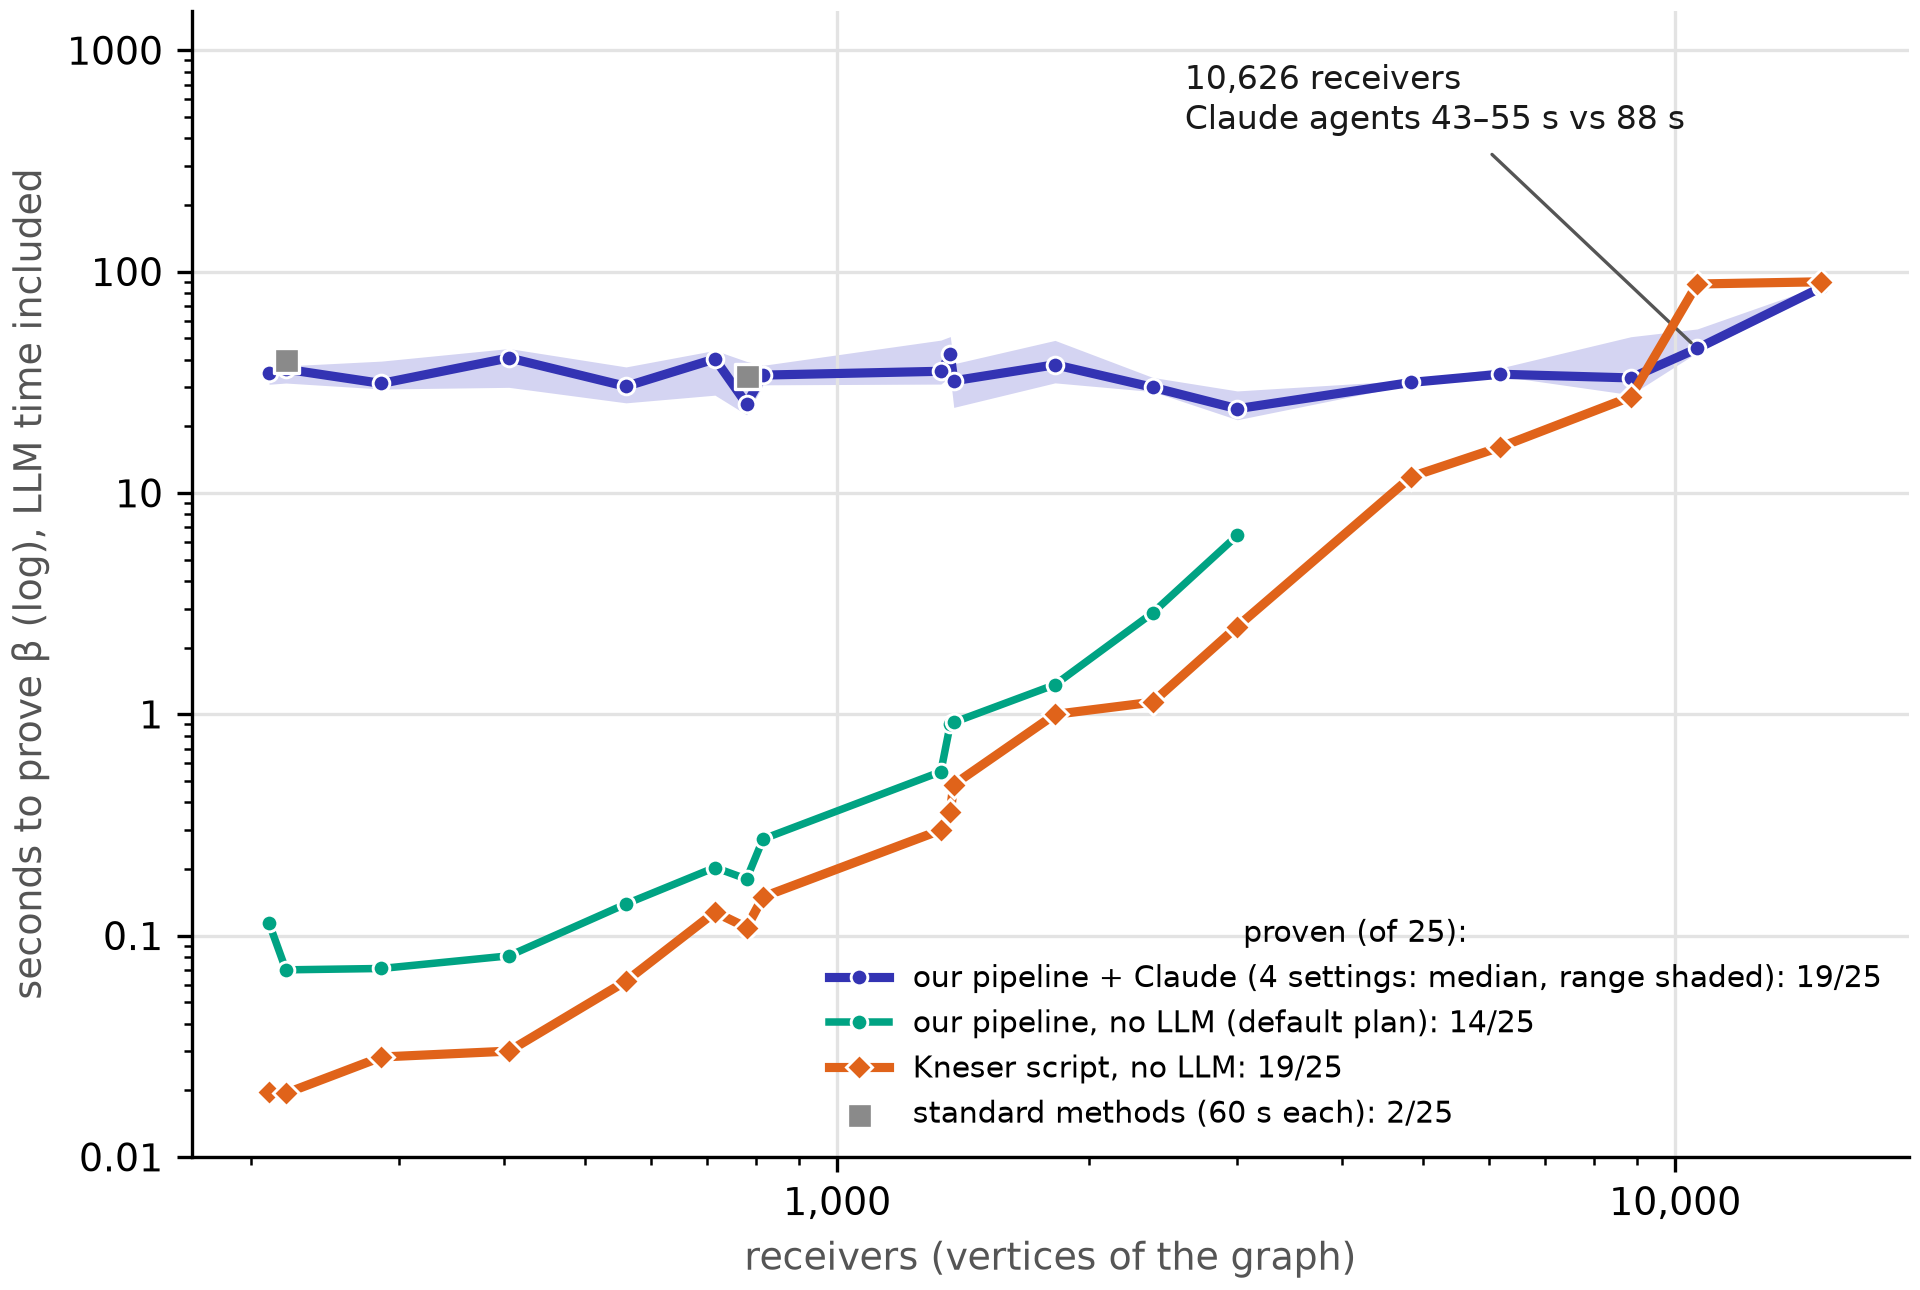
\includegraphics[width=0.82\textwidth]{fig/time_to_prove_beamer.png}
  \caption{Time to prove $\beta$ against the number of receivers (container, one CPU core per run, only proven graphs
  drawn): our pipeline with Claude (four settings), the same pipeline without an LLM (default plan), the no-LLM
  Kneser script, and the standard methods. Below about 9{,}000 receivers the script is faster; at 10{,}626 receivers
  the Claude agents need 43--55\,s against 88\,s, at 14{,}950 they need 81--87\,s against 90\,s. Without an LLM the
  default plan proves none of the five large graphs.}
  \label{fig:ttp}
\end{figure}

\begin{table}[ht]
  \centering\small
  \resizebox{\textwidth}{!}{\begin{tabular}{@{}lcccc@{}}
    \toprule
    & & & \multicolumn{2}{c}{Time at $N$ receivers} \\ \cmidrule(l){4-5}
    Method & Proven & Median time & 10{,}626 & 14{,}950 \\
    \midrule
    Standard methods (CP-SAT, covers, $\mathbb{F}_2$ SAT) & 2/25 & 40\,s & -- & -- \\
    Kneser script, no LLM & 19/25 & 0.36\,s & 87.9\,s & 89.9\,s \\
    \midrule
    Our pipeline, no LLM (default plan) & 14/25 & 0.24\,s & \makecell{open, $[1771,1948]$\\after 21.5\,s} & \makecell{open, $[2300,2529]$\\after 79.6\,s} \\
    \makecell[l]{Our pipeline, no LLM, fast path\\(GPU server; 23 graphs)} & 17/23 & 0.35\,s & not run & not run \\
    \midrule
    Our pipeline + Claude Sonnet 5.5 (medium) & 19/25 & 31.5\,s & 45.5\,s & 83.5\,s \\
    Our pipeline + Claude Opus 5.5 (low)      & 19/25 & 31.0\,s & 44.4\,s & 86.7\,s \\
    Our pipeline + Claude Opus 5.5 (medium)   & 19/25 & 35.9\,s & \textbf{43.1\,s} & \textbf{81.1\,s} \\
    Our pipeline + Claude Opus 5.5 (high)     & 19/25 & 38.3\,s & 55.0\,s & 86.2\,s \\
    \makecell[l]{Our pipeline + Qwen2.5-Coder-32B-AWQ\\(GPU server, vLLM)} & 17/23 & 40.9\,s & not run & not run \\
    \bottomrule
  \end{tabular}}
  \caption{Time to prove $\beta$ on the 25 graphs. Container, one core per run, unless stated. The LLM rows use one
  fresh agent per graph that is not given the graph's name. The Claude rows use prompt version v4; the Qwen row used
  prompt version v3 on older code (before plan-step results were shown to the agents). Each median is over the graphs
  that method proves, so medians of methods that prove different graphs are not comparable: the pipeline without an
  LLM (0.24\,s) proves only the 14 smaller graphs, and on every graph both prove the Kneser script is faster
  (Figure~\ref{fig:ttp}). The
  ``no LLM'' rows run the same pipeline: the default plan has no family hypothesis, and the opt-in fast path
  recognises $K(n,k)$ from the receiver count and degree (the \texttt{binomial\_match} tool) and applies the
  theorem; the fast path and Qwen ran on the GPU server on 23 of the 25 graphs (not the two largest). Haiku~5.5 was
  run in the blind ablation (Table~\ref{tab:blind}) and on only 2 of the 25 graphs here, so it has no row. Files: \file{kneser-agent/results/runs.jsonl} (tags
  \texttt{ctr}, \texttt{fastpath}, \texttt{<model>-full}) and \file{kneser-agent/results/baselines\_ctr\{,\_xl\}.jsonl};
  recomputed on 27 November.}
  \label{tab:ablation}
\end{table}

\begin{figure}[ht]
  \centering
  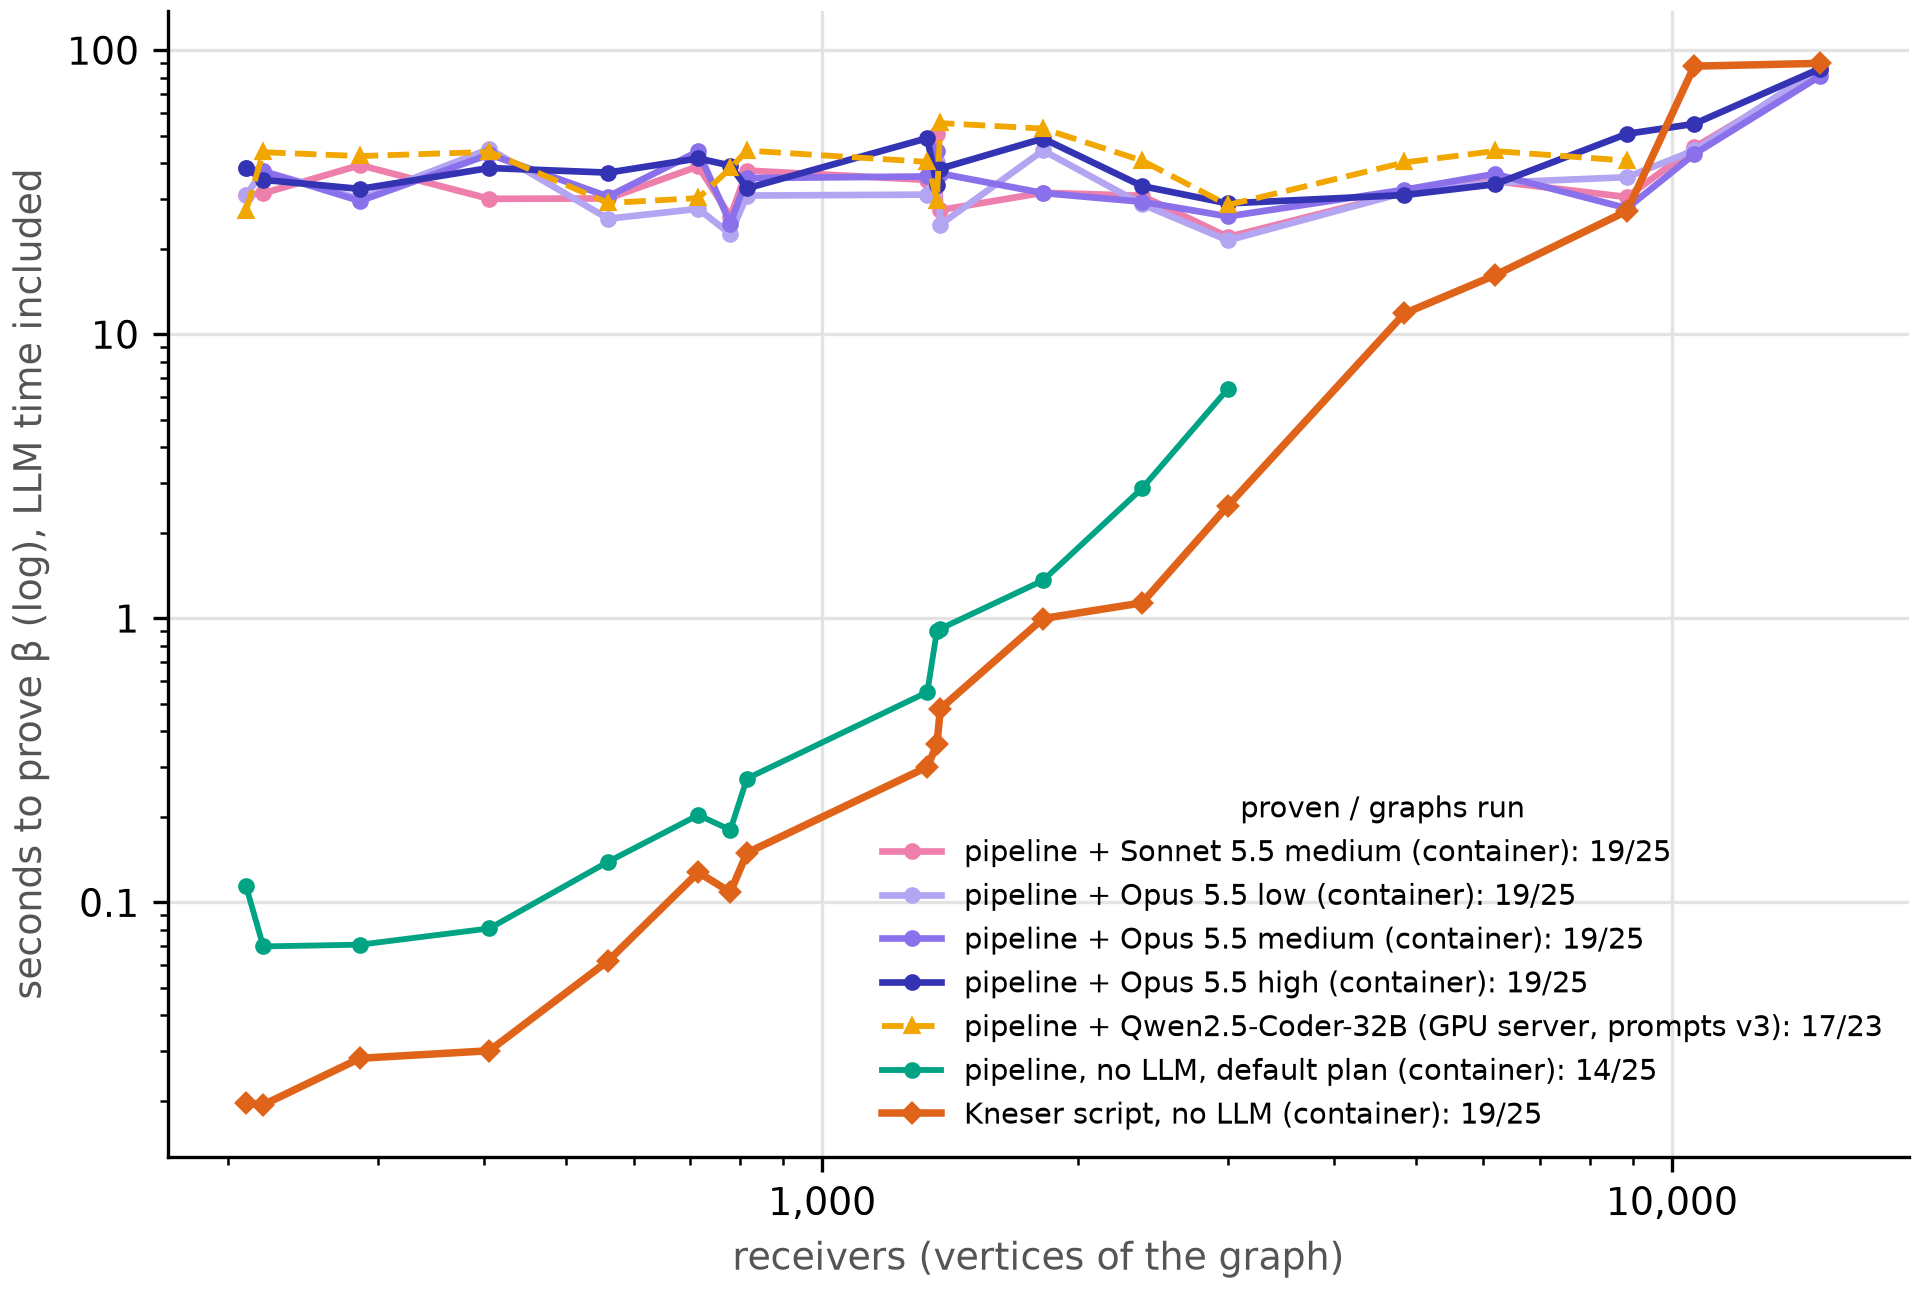
\includegraphics[width=0.78\textwidth]{fig/time_to_prove_models_beamer.png}
  \caption{Time to prove $\beta$ for each LLM driving the pipeline, the pipeline without an LLM, and the Kneser
  script; the legend gives proven graphs out of graphs run. The Claude, no-LLM and script lines use the protocol of
  Figure~\ref{fig:ttp} (container, one core). Qwen ran on the GPU server (vLLM, prompt version v3, cores shared with
  other users) on 23 of the 25 graphs, so its line is not directly comparable.}
  \label{fig:ttp-models}
\end{figure}

\textbf{What the results show, and what they do not.}
\begin{itemize}
  \item All four Claude settings and the Kneser script prove the same 19 graphs; more effort only adds time.
  \item The 6 graphs left open (the 3 exceptions of the theorem and the 3 perturbed or random controls) stay open for
  every method; no method claimed a false value, and every agent bound passed the independent verifier.
  \item \textbf{The LLM's contribution is recognising the family, and code does that too.} Without an LLM, the
  default plan proves the 14 regular Kneser graphs and none of the 5 large ones, because it never calls the family
  rule. With any Claude model the Solver names $K(n,k)$ and the family rule closes all five. But the opt-in fast path,
  a few lines of code with no LLM, recognises $K(n,k)$ the same way and proves every graph it was run on that the
  Claude agents prove (17 of 23). On this benchmark, which consists of Kneser graphs and close relatives, the LLM adds
  no proven graph over that rule and costs a median of 30\,s of LLM time per graph (12--50\,s over the 76
proven Claude runs).
  \item \textbf{The speed on large graphs comes from the rank engine, not the LLM.} The pipeline's rank engine stops
  once the rank is certified ($O(N^2r)$), while the Kneser script computes a full exact rank ($O(N^3)$). With the LLM
  the pipeline needs 43--55\,s at 10{,}626 receivers against the script's 88\,s, of which 28--42\,s is LLM time. The
  no-LLM fast path through the same engine is faster still: it proved $K(20,4)$, $K(17,5)$ and $K(23,4)$ in
  5.2--23.2\,s on 26 November and 2.5--10.0\,s in the 27 November rerun (Section~\ref{sec:gpubench}), against 28--51\,s for the Claude agents in the container; the machines
  differ, so this is indicative, and the fast path was not run at 10{,}626 or 14{,}950 receivers.
  \item \textbf{Where an LLM could matter, we have no evidence yet.} A plan written for the graph at hand should help
  on graphs that no fixed rule recognises. The benchmark has no such graph on which any method closes the bracket, so
  this remains a hypothesis.
\end{itemize}

\textbf{How blind the agent is.} ``Blind'' means only that the input contains no graph name and the vertices are
shuffled. Two limits follow. First, nothing sandboxed the Claude Code agents: the instruction of
Step~R\ref{st:agentrun} told each agent to run one command and read no other file, but no mechanism enforced it, and
an agent could in principle have read the repository (including the benchmark specification). Second, the models
know Kneser graphs from training, and $N=\binom nk$ with degree $\binom{n-k}{k}$ is a strong signature that a model
can match from memory. Recognising the family is therefore not evidence of reasoning about an unknown structure; the
fixed \texttt{binomial\_match} rule does the same. Every bound is still certified by code, so neither limit can make
a reported value wrong; they limit what the agent results say about the LLM.

\subsection{Earlier benchmark on the GPU server (26 Nov, Qwen2.5-Coder-32B)}\label{sec:gpubench}
GPU server, 64 cores shared with other users; baselines pinned to cores 16--27, agent runs to 28--31 (3 workers);
standard methods 120\,s each; agent budget 300\,s. These Qwen numbers use prompt version v3 on code before the plan-step
results were shown to the agents.
\begin{itemize}
  \item Proven exact, 20 benchmark graphs: standard methods 2, the Kneser script 14, agent without LLM 14, agent +
  Qwen 32B 14 (also 14 with generic rules only). All 14 are the regular Kneser graphs.
  \item Large graphs (4{,}845--8{,}855 receivers): the Kneser script 3/3, agent + Qwen with the rule 3/3, agent
  without LLM 0/3, agent + Qwen generic only 0/3, standard methods 0/3. In the default plan the family rule is reached
  only through an LLM hypothesis, and it is what closes these graphs; the opt-in fast path below reaches the same
  rule without an LLM.
  \item Speed: without an LLM the agent is slower than the Kneser script on the shared exact graphs (median time
  ratio \x0.61, by at most 0.6\,s), and \x135 faster than the standard methods on the 2 graphs they prove. On the large
  graphs the agent's compute time is 5--8\x{} lower (2.3 / 4.5 / 8.0\,s against 18.7 / 23.0 / 41.6\,s), but with LLM
  seconds its wall time is about 2\x{} longer on two of them and equal on $K(23,4)$. Qwen adds a median 43\,s of LLM
  time per run (max 56\,s).
  \item Fast path (opt-in, no LLM): recognising $K(n,k)$ from the receiver count and degree and applying the rule
  proves $K(20,4)$, $K(17,5)$, $K(23,4)$: the bracket closed at 5.2 / 15.0 / 23.2\,s on 26 November (the Kneser
  script: 18.7 / 23.0 / 41.6\,s) and at 2.5 / 5.3 / 10.0\,s in a rerun on 27 November (the row of
  Table~\ref{tab:ablation}); times from the run traces. Both are faster than the agent with Qwen and than the Claude
  agents in the container (28--51\,s).
  \item Losses: to the Kneser script, on time, on most small exact graphs (e.g.\ $K(21,2)$ 0.12\,s against 0.03\,s);
  never on accuracy. On the 3 exceptions both reach the same brackets ($[84,93]$, $[286,287]$, $[495,507]$); on the
  controls the agent's brackets are tighter ($K(16,4)$ minus 1\% of edges: $[455,534]$ against $[0,1818]$). The
  script's lower bound of 0 is what it reports, not a bound anyone would accept: on a graph it does not recognise it
  skips its greedy independent set, and its general solver returned no lower bound within the time limit. Any greedy
  independent set gives at least 1, and the agent's gives 455.
\end{itemize}

\subsection{Blind-agent ablation: what the model changes}
\begin{figure}[ht]
  \centering
  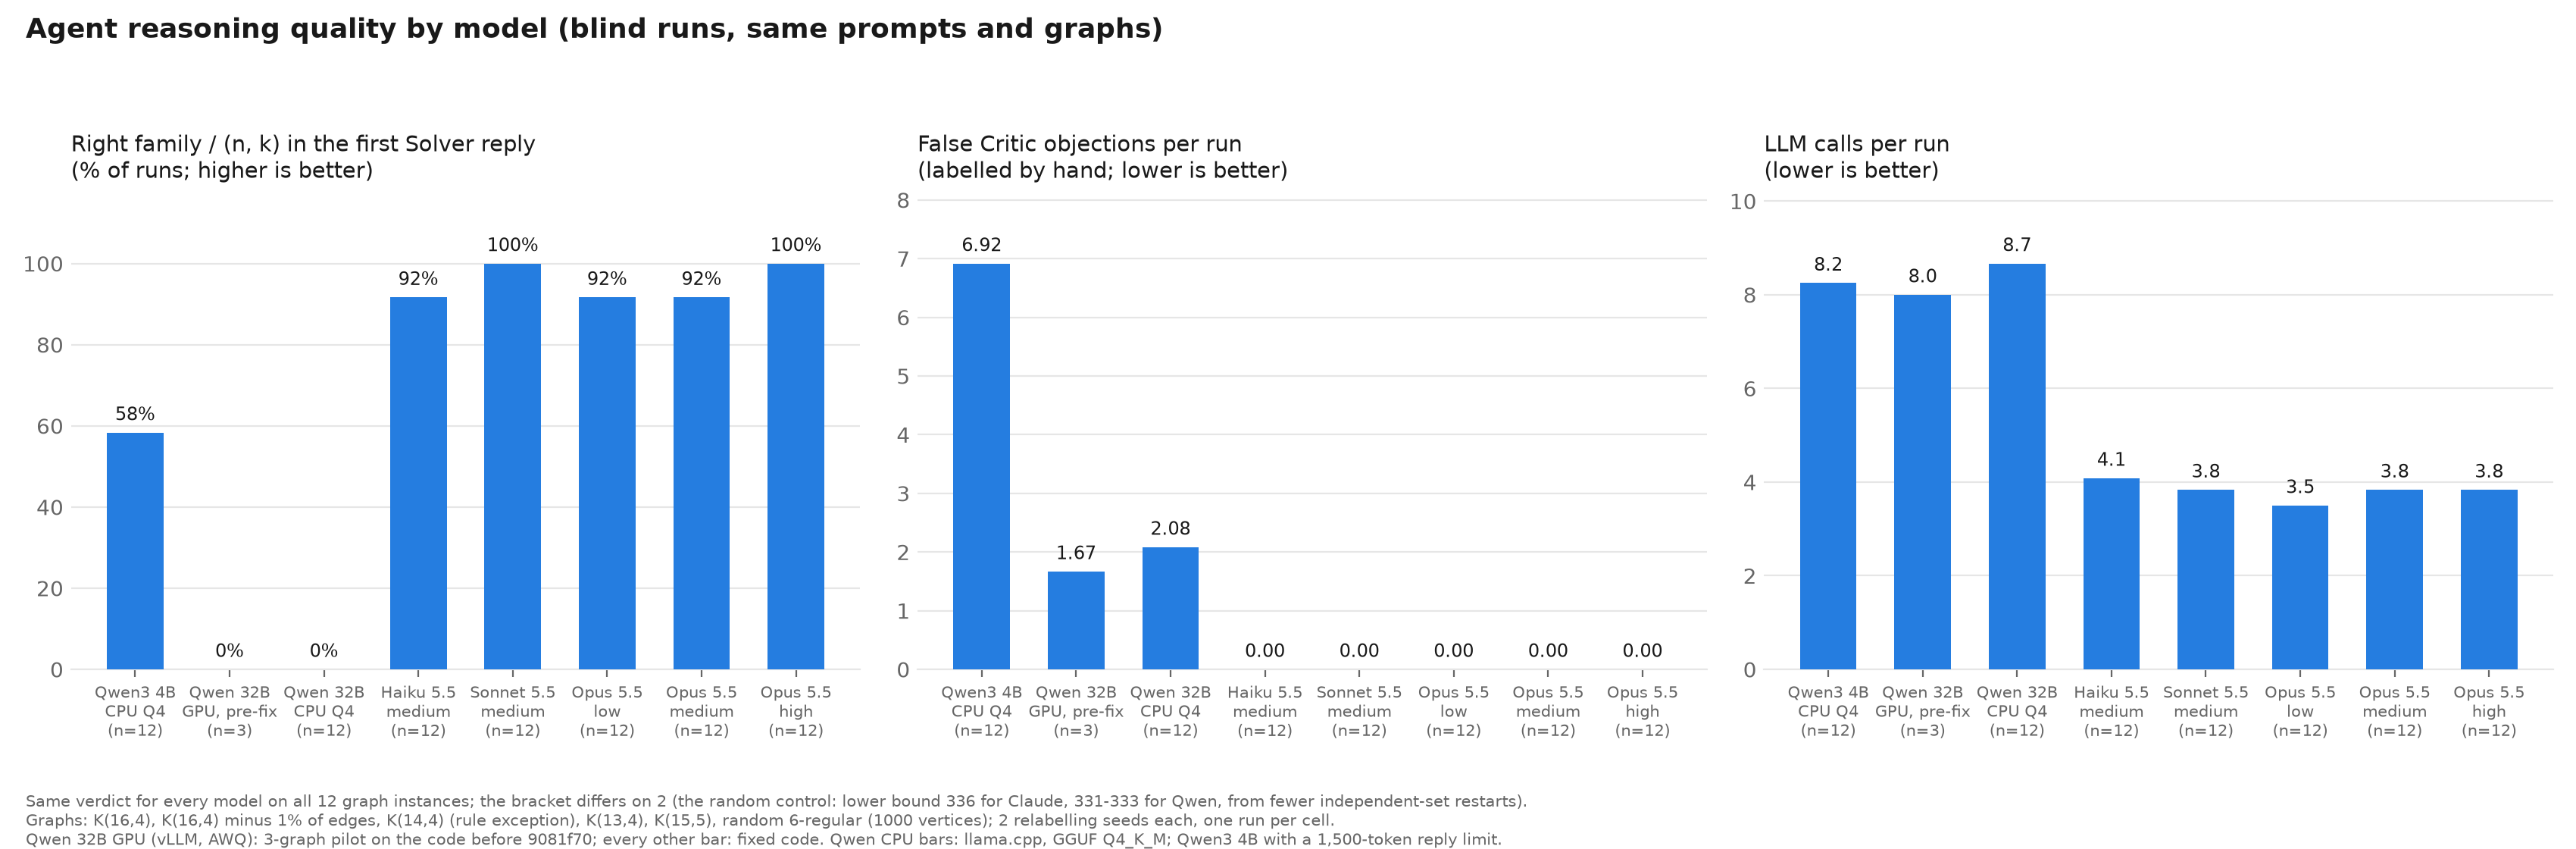
\includegraphics[width=\textwidth]{fig/model_ablation.png}
  \caption{Reasoning quality by model on 6 graphs \x{} 2 relabelling seeds = 12 cells, one blind run per cell:
  $K(16,4)$, $K(16,4)$ minus 1\% of edges, $K(14,4)$ (rule exception), $K(13,4)$, $K(15,5)$ and a random 6-regular
  graph on 1{,}000 vertices.}
  \label{fig:ablation}
\end{figure}

\begin{table}[ht]
  \centering\small
  \begin{tabular}{@{}>{\raggedright\arraybackslash}p{6.4cm}ccc@{}}
    \toprule
    Model & \makecell{False Critic\\objections per run} & \makecell{Right family in\\first Solver reply} & \makecell{LLM calls\\per run} \\
    \midrule
    Claude (Haiku 5.5 medium, Sonnet 5.5 medium, Opus 5.5 low/medium/high) & 0 (in 60 runs) & 11--12 of 12 & 3.5--4.1 \\
    Qwen2.5-Coder-32B (CPU, llama.cpp) & 2.08 & 0 of 12 & 8.7 \\
    Qwen2.5-Coder-32B (GPU pilot, earlier code, 3 runs) & 1.67 & 0 of 3 & 8.0 \\
    Qwen3-4B (CPU, 1{,}500-token limit) & 6.92 & 7 of 12 & 8.2 \\
    \bottomrule
  \end{tabular}
  \caption{Blind-agent ablation (values of Figure~\ref{fig:ablation}).}
  \label{tab:blind}
\end{table}

Every model reaches the same verdict on every graph instance and the same bracket on the 10 Kneser-type instances;
on the random control the lower bound differs (Claude 336, Qwen 331--333) because the Claude Solvers asked for
200--1{,}000 independent-set restarts and Qwen for 10. The model changes the dialogue and its cost, and only through
its plan the bound, never the correctness. Every objection was labelled with a reason by a fixed rule. Qwen3-4B at
the default 600-token limit had its JSON cut off in 26 of 48 requests, hence the 1{,}500-token rerun.

% ---------------------------------------------------------------------------------------------------- 10
\section{Reproducing Part II step by step}\label{sec:repro2}

The steps continue the numbering of Section~\ref{sec:repro1}. Everything in this part runs on CPUs; only the
optional local LLM (Qwen) needs a GPU. Additional software: \texttt{python-flint} (exact ranks over $\Fp$),
\texttt{numba}, \texttt{ortools} 9.15 (CP-SAT), \texttt{python-sat} 1.9, \texttt{networkx} 3.7, the SAT solver
CaDiCaL~\cite{cadical} and the proof checker drat-trim~\cite{drattrim}, and for the local LLM vLLM~\cite{vllm} (GPU)
or llama.cpp~\cite{llamacpp} build b12780 (CPU). The files
are listed in Appendix~\ref{app:map}.

\subsection{The theorem}

\begin{step}{st:rank}{Check Theorem~\ref{thm:rank} by exact ranks}
\begin{enumerate}
  \item For every $k\ge2$, $n>2k$ with $\binom nk\le2000$ and every prime $p$ in the range checked, build the
  $\binom nk\times\binom nk$ matrix $H_{A,B}=\binom{|A\cap B|-1}{k-1} \bmod p$ (equivalently $I+\varepsilon D$ with
  $\varepsilon=(-1)^{k-1}$), indexed by the $k$-subsets of $\{1,\dots,n\}$.
  \item Compute $\operatorname{rank}_p H$ exactly (FLINT \texttt{nmod\_mat}) and compare ``rank $=\binom{n-1}{k-1}$''
  with ``$q_p(k)\mid n-2k$'', where $q_p(k)$ is the least power of $p$ that is $\ge k$.
  \item For the same cases check the decoding identity directly: for every row $A'\not\ni1$, compare $H[A',:]$ with
  $\varepsilon\sum_{A\ni1,\,A\cap A'=\emptyset}H[A,:]$ modulo $p$.
  \item Check the $k+1$ congruences of step~3 of the proof for $m=n-2k$ up to 400, $k\le12$, $p\le13$, against
  $q_p(k)\mid m$.
\end{enumerate}
\chk{318 $(n,k,p)$ cases, the three statements agree in every case, no exception.}
\end{step}

\begin{step}{st:indep}{Cross-check with an independent rank code}
On 82 cases ($\binom nk\le3500$, $k\le6$; 39 with $k\nmid n$) recompute every rank with a separately written
Gaussian elimination modulo $p$ that shares no code with FLINT, and check that $H$ fits $K(n,k)$ (nonzero diagonal,
zero on every non-adjacent pair) and that $H$ is the identity on the star.
\chk{both rank codes agree on all 82 cases.}
\end{step}

\begin{step}{st:secondproof}{Second proof by integer diagonal forms}
Using the Smith/diagonal form of the subset-intersection matrices of Ducey et al.~\cite{ducey}, compute for each
$(n,k,p)$ the predicted $p$-rank of $H$ and compare it with Theorem~\ref{thm:rank}, for $k\le12$, $n\le120$, $p\le13$
(every prime including $p\le k$). Separately verify the $k=3$ proof by inclusion matrices step by step for $n\le22$
and the primes up to 23.
\chk{6{,}666 cases agree.}
\end{step}

\begin{step}{st:codecheck}{Check the explicit code}
For $K(7,2)$ over $\mathbb{F}_3$ (and any case with $q\mid n-2k$): draw random messages $x_B\in\Fp$ for all $k$-sets,
compute the $\alpha$ broadcasts $y_A=x_A+\varepsilon\sum_{B\cap A=\emptyset}x_B$ for $A\ni1$, and let every receiver
decode as in Theorem~\ref{thm:code} using only its side information. Every receiver must recover its message.
\end{step}

\begin{step}{st:sat}{Lower bounds over $\mathbb{F}_2$ by SAT, checked with DRAT}
\begin{enumerate}
  \item Encode ``$\operatorname{minrk}_2(G)\le r$'' as CNF: variables $u_{ik},v_{jk}$ for the factors $U,V\in
  \mathbb{F}_2^{N\times r}$ of $M=UV^\top$; for every constrained entry (diagonal or non-adjacent pair) an AND gate
  $z_k=u_{ik}\wedge v_{jk}$ per coordinate and an XOR chain over $k$, with the final value forced to 1 on the diagonal
  and 0 on non-adjacent pairs; entries on edges are unconstrained. Break the $GL(r,\mathbb{F}_2)$ symmetry by fixing
  $u_0=e_1$ (sound because $M_{00}=1$); in the family runs also fix the rows of a known independent set (proved sound
  and tested against brute force on small graphs).
  \item Solve with CaDiCaL, asking it to write a DRAT proof when the answer is UNSAT; then check the proof against the
  exact CNF with drat-trim. Only a VERIFIED check counts as a proof.
\end{enumerate}
\chk{$K(7,2)$, $r=6$: UNSAT, VERIFIED in 0.39\,s. $K(7,3)$ at $r=17$ and $K(8,3)$ at $r=21$: UNSAT, VERIFIED ($K(8,3)$:
solve 950\,s, check 1{,}663\,s), so $\operatorname{minrk}_2=18$ and 22 together with the matching codes.}
\end{step}

\subsection{The agent}

\begin{step}{st:graphs}{Build the benchmark graphs}
\begin{enumerate}
  \item $K(n,k)$: vertices are the $k$-subsets of $\{1,\dots,n\}$, edges join disjoint subsets. Store only the
  boolean adjacency matrix.
  \item Relabel the vertices with a random permutation of seed $s$ (seed 0 for Table~\ref{tab:ablation}, seeds 0 and
  1 for the blind ablation); the agent never receives the graph's name.
  \item Controls: delete 1\% of the edges of $K(16,4)$ and $K(18,3)$ uniformly at random; a random 6-regular graph on
  1{,}000 vertices.
  \item The 25 graphs of Section~\ref{sec:agentres}, with their known $\beta$ or bracket as ground truth.
\end{enumerate}
\end{step}

\begin{step}{st:baselines}{Run the baselines}
Pin every run to one CPU core with \texttt{OMP\_NUM\_THREADS=1}.
\begin{itemize}
  \item \textbf{Standard methods}, each in its own process with one thread and 60\,s: maximum independent set by
  CP-SAT (lower bound); clique cover by CP-SAT, fractional clique cover, and $\mathbb{F}_2$ minrank by the SAT encoding
  of Step~R\ref{st:sat} (upper bounds). A graph is proven when the best lower bound equals the best upper bound.
  \item \textbf{Kneser agent (no LLM)}: the five steps of Figure~\ref{fig:baseline}, with a limit of 120\,s on the two
  largest graphs.
\end{itemize}
\end{step}

\begin{step}{st:agentrun}{Run the agent on every graph}
\begin{enumerate}
  \item Pin the run to one core; the scheduler's 3 workers share it. Warm up the numba rank kernel before the run
  clock starts. Budget 300\,s.
  \item Choose the LLM backend: \emph{none} (a deterministic default plan, no LLM); \emph{local} (an
  OpenAI-compatible endpoint, e.g.\ vLLM serving \texttt{Qwen/Qwen2.5-Coder-32B-Instruct-AWQ} on one A6000, or
  llama.cpp with a Q4\_K\_M GGUF on CPU cores, JSON mode on); or \emph{file-based}, where the pipeline writes each
  request (system prompt + input) as a JSON file and waits for the reply file.
  \item For the Claude results, answer the file-based requests with a fresh Claude Code agent of the stated model
  and effort, started once per graph with only this instruction (folder filled in):
  \begin{quote}\small
  ``You are acting as the language model behind a running software pipeline. You have no other context, and you must
  not look for any: reason independently and autonomously, only from the data in each request. The ONLY command you
  may run is \texttt{python3 next\_req.py <folder>}. The ONLY file operation you may do is writing reply files into
  that same folder. Do not read, list, search or open any other file or directory, do not run any other command, do
  not use web search or fetch. Do not write code to compute anything; think it through yourself. Loop: run the
  command; on DONE stop; otherwise treat "system" as your instructions and "prompt" as the input, produce exactly the
  reply the system text asks for (one JSON object), write it to \texttt{<folder>/rep\_<id as 3 digits>.json}, repeat.''
  \end{quote}
  This instruction is the only safeguard: nothing sandboxes the agent, so it could read other files. To make
  ``blind'' enforced rather than requested, run each agent in a container or directory that holds only the request
  folder and \texttt{next\_req.py} (we did not do this; Section~\ref{sec:agentres}).
  \item Record per run: verdict, final bracket $[L,U]$, every verifier check, the wall time until $L=U$ first held
  (LLM time included), and the full trace.
\end{enumerate}
\end{step}

\begin{step}{st:score}{Score the runs}
A graph counts as proven when the verdict is ``proven'', $L=U$, and all verifier checks pass. For each configuration
report the number proven, the median time over proven graphs, and the times at 10{,}626 and 14{,}950 receivers.
Also run the pipeline with backend \emph{none}, once with the default plan and once with the opt-in fast path, so the
LLM rows can be compared with the same pipeline without an LLM.
\chk{Table~\ref{tab:ablation}: 19/25 for every Claude setting and for the Kneser script, 14/25 for the pipeline
without an LLM (default plan), 17/23 with the fast path, 2/25 for the standard methods. Times depend on the machine and, for the LLM, on the provider's latency; the counts and brackets do not.}
\end{step}

\begin{step}{st:blind}{Blind-agent ablation}
Run the 6 graphs of Figure~\ref{fig:ablation} with relabelling seeds 0 and 1 (12 cells) once per model
configuration. From each trace count the LLM calls, check whether the first Solver reply names the right family and
$(n,k)$, and label every Critic objection with a fixed rule: an objection is \emph{false} if it asserts something
wrong about the data or the tools, including a wrong inference (e.g.\ ``\texttt{family\_rule} returned null, so
$K(14,4)$ is not confirmed'': a rule naming no field says nothing about the family); a true statement, even an
irrelevant one, and a pure process request (``query X first'') are not false. Average per run.
\chk{Table~\ref{tab:blind}.}
\end{step}

\begin{step}{st:tests}{Unit tests}
Run the test suite of the agent: the rank engine against FLINT and against the verifier's own elimination on random
matrices, the evidence validation, and a test asserting that the verifier imports nothing from the tools or the rank
engine. All must pass.
\end{step}

% ---------------------------------------------------------------------------------------------------- 11
\section{Conclusions}\label{sec:conclusions}
\begin{itemize}
  \item \textbf{Early exit.} The fastest rule changes with batch size and input length; a rule derived from the
  measured cost tracks it. At matched accuracy it leads on QQP (2--17\% on the GTX 1650 cost table; 8--14\% timed on
  the A6000, replaying recorded decisions on a random-weight network) and on Llama classifiers with trained weights
  (3.66\x). Certified selection keeps the one-point budget on re-splits. The slowdown bound is proved for the trimmed
  collective stop and held empirically for the full rule in every tested batch. No gain on RoBERTa MNLI or on LLM
  decoders, and the accuracy loss lands on hard inputs.
  \item \textbf{Minrank.} $\operatorname{rank}_{\Fp}(I+\varepsilon D)=\binom{n-1}{k-1}$ exactly when $q_p(k)\mid n-2k$.
  Hence, whenever $q_p(k)\mid n-2k$, $\operatorname{minrk}_{\Fp}(K(n,k))=\beta=\alpha$ with an explicit optimal
  index code; this is new for $k\nmid n$. The converse does not hold for the minrank: $K(9,3)$ over $\mathbb{F}_2$ has
  $\operatorname{minrk}=\alpha$ by Baranyai's theorem although $4\nmid3$. Small cases such as $K(9,2)$ over
  $\mathbb{F}_2$ remain open.
  \item \textbf{Agent.} A Solver--Critic--Verifier pipeline, not given the graph's name, proves $\beta$ on 19 of 25
  graphs with each of the four Claude settings run on the full benchmark; the no-LLM Kneser script also proves 19. The
  LLM's measurable contribution is recognising the Kneser family, which a no-LLM fast path also does (17 of the 23
  graphs it ran on, all that the Claude agents prove there). The pipeline's speed on large graphs (43--55\,s against
  88\,s at 10{,}626 receivers) comes from its $O(N^2r)$ rank engine; the LLM adds a median of 30\,s per graph (12--50\,s). Whether an LLM
  helps on graphs that no fixed rule recognises is untested.
\end{itemize}

% ---------------------------------------------------------------------------------------------------- references
\begin{thebibliography}{99}\small
\bibitem{deebert} J.~Xin, R.~Tang, J.~Lee, Y.~Yu, J.~Lin. DeeBERT: Dynamic Early Exiting for Accelerating BERT Inference. ACL 2020.
\bibitem{pabee} W.~Zhou, C.~Xu, T.~Ge, J.~McAuley, K.~Xu, F.~Wei. BERT Loses Patience: Fast and Robust Inference with Early Exit. NeurIPS 2020.
\bibitem{drex} X.~Liu et al. Dynamic Rebatching for Efficient Early-Exit Inference with DREX. arXiv:2512.15705, 2025.
\bibitem{geep} L.~Li et al. Accelerating BERT Inference with GPU-Efficient Exit Prediction. Frontiers of Computer Science 18(3), 2024.
\bibitem{miao} R.~Miao, Y.~Yan, X.~Yao, T.~Yang. An Efficient Inference Framework for Early-exit Large Language Models. arXiv:2407.20272, 2024.
\bibitem{apparate} Y.~Dai, R.~Pan, A.~Iyer, K.~Li, R.~Netravali. Apparate: Rethinking Early Exits to Tame Latency-Throughput Tensions in ML Serving. SOSP 2024.
\bibitem{fastsafe} M.~Jazbec, A.~Timans, et al. Fast yet Safe: Early-Exiting with Risk Control. NeurIPS 2024.
\bibitem{e3} A.~Iyer et al. Improving DNN Inference Throughput Using Practical, Per-Input Compute Adaptation (E3). SOSP 2024.
\bibitem{sloth} S.~Hong, Y.~Kaya, I.-V.~Modoranu, T.~Dumitra\c{s}. A Panda? No, It's a Sloth: Slowdown Attacks on Adaptive Multi-Exit Neural Network Inference. ICLR 2021.
\bibitem{lostpatience} Z.~Coalson, G.~Ritter, R.~Bobba, S.~Hong. BERT Lost Patience Won't Be Robust to Adversarial Slowdown. NeurIPS 2023.
\bibitem{falsesense} Y.~Chen et al. Dynamic Transformers Provide a False Sense of Efficiency. ACL 2023.
\bibitem{chow} Y.~S.~Chow, H.~Robbins, D.~Siegmund. \emph{Great Expectations: The Theory of Optimal Stopping}. Houghton Mifflin, 1971.
\bibitem{ltt} A.~N.~Angelopoulos, S.~Bates, E.~J.~Cand\`es, M.~I.~Jordan, L.~Lei. Learn then Test: Calibrating Predictive Algorithms to Achieve Risk Control. arXiv:2110.01052, 2021.
\bibitem{labeleff} N.~Cesa-Bianchi, G.~Lugosi, G.~Stoltz. Minimizing Regret with Label Efficient Prediction. IEEE Trans.\ Information Theory 51(6), 2005.
\bibitem{ceebert} D.~J.~Bajpai, M.~K.~Hanawal. CeeBERT: Cross-Domain Inference in Early Exit BERT. Findings of ACL 2024.
\bibitem{ucbee} R.~G.~Pacheco et al. UCBEE: A Multi-Armed Bandit Approach for Early-Exit in Neural Networks. IEEE Trans.\ Network and Service Management, 2024.
\bibitem{roberta} Y.~Liu et al. RoBERTa: A Robustly Optimized BERT Pretraining Approach. arXiv:1907.11692, 2019.
\bibitem{mnli} A.~Williams, N.~Nangia, S.~Bowman. A Broad-Coverage Challenge Corpus for Sentence Understanding through Inference. NAACL 2018.
\bibitem{glue} A.~Wang et al. GLUE: A Multi-Task Benchmark and Analysis Platform for Natural Language Understanding. ICLR 2019.
\bibitem{vit} A.~Dosovitskiy et al. An Image Is Worth 16x16 Words: Transformers for Image Recognition at Scale. ICLR 2021.
\bibitem{cifar} A.~Krizhevsky. Learning Multiple Layers of Features from Tiny Images. Tech.\ report, University of Toronto, 2009.
\bibitem{qwen} Qwen Team. Qwen2.5 Technical Report. arXiv:2412.15115, 2024.
\bibitem{llama} Llama Team, Meta AI. The Llama 3 Herd of Models. arXiv:2407.21783, 2024.
\bibitem{wikitext} S.~Merity, C.~Xiong, J.~Bradbury, R.~Socher. Pointer Sentinel Mixture Models. ICLR 2017.
\bibitem{skipdecode} L.~Del Corro et al. SkipDecode: Autoregressive Skip Decoding with Batching and Caching for Efficient LLM Inference. arXiv:2307.02628, 2023.
\bibitem{layerskip} M.~Elhoushi et al. LayerSkip: Enabling Early Exit Inference and Self-Speculative Decoding. ACL 2024.
\bibitem{calm} T.~Schuster et al. Confident Adaptive Language Modeling. NeurIPS 2022.
\bibitem{baryossef} Z.~Bar-Yossef, Y.~Birk, T.~S.~Jayram, T.~Kol. Index Coding with Side Information. IEEE Trans.\ Information Theory 57(3), 2011.
\bibitem{gh} A.~Golovnev, I.~Haviv. The (Generalized) Orthogonality Dimension of (Generalized) Kneser Graphs: Bounds and Applications. Theory of Computing, 2022.
\bibitem{ducey} J.~E.~Ducey, L.~Engelthaler, J.~Gathje, B.~Jones, I.~Pfaff, J.~Plute. Integer Diagonal Forms for Subset Intersection Relations. arXiv:2310.09227, 2023.
\bibitem{rcps} S.~Bates, A.~Angelopoulos, L.~Lei, J.~Malik, M.~I.~Jordan. Distribution-Free, Risk-Controlling Prediction Sets. Journal of the ACM 68(6), 2021 (Hoeffding--Bentkus bound).
\bibitem{wsr} I.~Waudby-Smith, A.~Ramdas. Estimating Means of Bounded Random Variables by Betting. Journal of the Royal Statistical Society Series B 86(1), 2024.
\bibitem{lora} E.~J.~Hu, Y.~Shen, P.~Wallis, Z.~Allen-Zhu, Y.~Li, S.~Wang, L.~Wang, W.~Chen. LoRA: Low-Rank Adaptation of Large Language Models. ICLR 2022.
\bibitem{funsearch} B.~Romera-Paredes et al. Mathematical Discoveries from Program Search with Large Language Models. Nature 625, 2024.
\bibitem{baranyai} Zs.~Baranyai. On the Factorization of the Complete Uniform Hypergraph. In \emph{Infinite and Finite Sets}, Colloq.\ Math.\ Soc.\ J\'anos Bolyai 10, North-Holland, 1975.
\bibitem{ekr} P.~Erd\H{o}s, C.~Ko, R.~Rado. Intersection Theorems for Systems of Finite Sets. Quarterly Journal of Mathematics 12(1), 1961.
\bibitem{lucas} E.~Lucas. Th\'eorie des fonctions num\'eriques simplement p\'eriodiques. American Journal of Mathematics 1, 1878.
\bibitem{cpsat} L.~Perron, F.~Didier. CP-SAT. Google OR-Tools, \url{https://developers.google.com/optimization}.
\bibitem{cadical} A.~Biere, T.~Faller, K.~Fazekas, M.~Fleury, N.~Froleyks, F.~Pollitt. CaDiCaL 2.0. CAV 2024.
\bibitem{drattrim} N.~Wetzler, M.~J.~H.~Heule, W.~A.~Hunt. DRAT-trim: Efficient Checking and Trimming Using Expressive Clausal Proofs. SAT 2014.
\bibitem{flint} The FLINT team. FLINT: Fast Library for Number Theory. \url{https://flintlib.org}.
\bibitem{tabucol} A.~Hertz, D.~de~Werra. Using Tabu Search Techniques for Graph Coloring. Computing 39(4), 1987.
\bibitem{vllm} W.~Kwon et al. Efficient Memory Management for Large Language Model Serving with PagedAttention. SOSP 2023.
\bibitem{llamacpp} G.~Gerganov et al. llama.cpp. \url{https://github.com/ggml-org/llama.cpp}.
\end{thebibliography}

% ==================================================================================================== appendices
\appendix
\section{Environment, versions and seeds}\label{app:env}

\begin{table}[ht]
  \centering\small
  \begin{tabularx}{\textwidth}{@{}>{\raggedright\arraybackslash}p{3.6cm}X@{}}
    \toprule
    Item & Value \\
    \midrule
    Repository & \repo, branch \texttt{main}, commit \texttt{50f1ef4} (the progress report of 13 November is commit \texttt{14e5bfa}) \\
    GPU server & Linux 6.8.0-151-generic; 2\x{} Intel Xeon Silver 4216 (64 threads); 4\x{} RTX A6000 (48\,GB) and 2\x{} RTX 3080 Ti (every server number in this report is from an RTX A6000); NVIDIA driver 580.159.04, CUDA 13.0 \\
    Laptop (Tables~\ref{tab:cost}--\ref{tab:summary}) & GTX 1650 4\,GB, fp32, 4 CPU threads; package versions not recorded \\
    Agent container (Table~\ref{tab:ablation}) & 4-core container; each pipeline pinned to one core (\texttt{taskset}, \texttt{OMP\_NUM\_THREADS=1}) \\
    Python & 3.12.3 in a virtual environment \\
    Key packages & torch 2.14.0+cu130, transformers 5.17.0, datasets 5.0.1, accelerate 1.15.0, numpy 2.5.3, scipy 1.18.1, pandas 3.0.6, scikit-learn 1.9.1, matplotlib 3.11.2, ortools 9.15.6755, python-sat 1.9.dev24, networkx 3.7, cvxpy 1.9.3, highspy 1.16.0, python-flint, numba \\
    Exact versions & \file{requirements-lock.txt} (\texttt{pip freeze} of the environment used for every run) \\
    External binaries & CaDiCaL and drat-trim (DRAT checks); vLLM and llama.cpp b12780 (local LLMs) \\
    \bottomrule
  \end{tabularx}
  \caption{Hardware and software.}
\end{table}

\textbf{Seeds.}
\begin{itemize}
  \item Training: seed 0 for every model (data order and initialisation of new heads). Tuning/held-out split of each
  trace: a permutation with seed 0.
  \item Selection: fit/cert split with seed 0; disjoint batches with seeds $B$ (fit), $B+1$ (cert), $B+2$ (old
  protocol), $100+B$ (held-out). Random-weight timing network: \texttt{torch.manual\_seed(0)}.
  \item Re-splits: seeds 0--29 (permutation seed $1000+s$, test batches $s+7$). Bandit: seeds 0--9. Load traces: 3
  arrival seeds. Random-search candidates: seed 0.
  \item Agent: the seed sets the vertex relabelling (seed 0 for Table~\ref{tab:ablation}; seeds 0 and 1 for the blind
  ablation).
  \item CPU reproductions were run with \texttt{PYTHONHASHSEED=0} and no visible GPU.
\end{itemize}

\textbf{Fine-tuned checkpoints} are not in the repository (they are large); Step~R\ref{st:train} retrains them. The
validation traces and all measured cost tables are committed, so every CPU step runs without checkpoints.

% ----------------------------------------------------------------------------------------------------
\section{Known issues and corrections}\label{app:issues}
\begin{itemize}
  \item \textbf{Calibration-cache bug (fixed 26 November).} The cost rule's calibration table was cached under the
  memory address of the trace object it was fitted on. In the re-split experiments new traces are built for every
  job; after garbage collection a later job could get the same address and reuse a table fitted on another re-split.
  Only the cost-rule rows of Tables~\ref{tab:resplit} and~\ref{tab:cert} were affected, and the result depended on
  the number of worker processes. The fix keeps a weak reference and refits when the object differs; runs with 3 and
  6 workers now give identical files. No claim changed status. This report shows the fixed values, with the 13
  November values of Table~\ref{tab:resplit} in brackets.
  \item \textbf{Labelling of Tables~\ref{tab:t11}--\ref{tab:t12b}.} These timings replay the trained model's recorded
  decisions on a random-weight fp32 network with random token ids, as on the GTX 1650. Accuracy is exact and timing
  does not depend on weights, but they are not ``trained checkpoint, real inputs'' timings as first labelled.
  Tables~\ref{tab:t15}--\ref{tab:t16} do use trained weights and real prompts.
  \item \textbf{Ten numbers in the 13 November text do not match the committed result files} (two in
  Table~\ref{tab:corrections}, the rest in the running text; none in a table of measurements, and none changes a
  claim). For one of them the file changed after 13 November: the CIFAR-100 robust-rule speedup (1.12\x{} in the
  text) is now a 22 November rerun giving 1.24\x, so the 13 November number may have matched the file of that day.
  Another, the simulator error of 15--32\%, cannot be traced to any file. All are corrected in Part~I and marked with
  footnotes: the simulator error of Table~\ref{tab:corrections} (now the per-policy 1--47\% of the files) and its
  1.12\x{} (file: 1.24\x); the heads' share under CUDA graphs (19\% on MNLI only, 12\%
  on QQP); the single-run bandit slopes (superseded by ten seeds); consensus collapsing at $k=1$ (only on CIFAR-100);
  the frozen Llama heads (8.2 points short, not about 5); and the 5.6 of the LLM ``Expected'' paragraph (4.0).
  \item \textbf{Not run:} the certified CUDA-graph tables (Section~\ref{sec:server-cert}), ViT at $B=16,64,128$, and
  trained checkpoints on the GTX 1650.
\end{itemize}

% ----------------------------------------------------------------------------------------------------
\section{The agents' system prompts (verbatim, prompt version v4)}\label{app:prompts}
The LLM chooses and orders tools, argues and explains; it never writes a bound.

\subsection*{Solver}
\lstinputlisting{prompts/solver.txt}
\subsection*{Critic and checkpoint}
\lstinputlisting{prompts/critic.txt}
\subsection*{Verifier}
\lstinputlisting{prompts/verifier.txt}
\subsection*{Tool list appended to the Solver and Critic prompts}
\lstinputlisting{prompts/tools.txt}

% ----------------------------------------------------------------------------------------------------
\section{Implementation map: where each step is in the repository}\label{app:map}

All paths are relative to the root of \repo{} (branch \texttt{main}, commit \texttt{50f1ef4}), except the sources
of this report, which are not in that commit (last row). To get the code and the environment:
\begin{lstlisting}[language=bash]
git clone https://github.com/yneha3229/Optimal-Batch-Level-Early-Exit.git
cd Optimal-Batch-Level-Early-Exit && git checkout 50f1ef4
python3.12 -m venv venv && venv/bin/pip install -r requirements-lock.txt
\end{lstlisting} Every result file named in the captions of this report is committed
under \file{results/} (Part~I) or \file{kneser-agent/results/} and \file{minrank/results/} (Part~II), with its raw
log under \file{logs/}.

{\small
\renewcommand{\arraystretch}{1.15}
\begin{longtable}{@{}>{\raggedright\arraybackslash}p{3.7cm}>{\raggedright\arraybackslash}p{11.9cm}@{}}
  \toprule
  Step & Implementation (files) \\
  \midrule
  \endhead
  \multicolumn{2}{@{}l}{\textbf{Part I: batch-level early exit}} \\
  R\ref{st:train} Fine-tune with exits & \file{traces/train\_exits.py} (training loop, loss, optimiser);
    \file{simulator/exit\_model.py} (exit heads, model wrapper); \file{configs/train\_\{mnli,qqp,cifar100\}.yaml}
    (hyperparameters); wrappers \file{scripts/train\_text.sh}, \file{scripts/train\_vision.sh} \\
  R\ref{st:traces} Record traces & \file{traces/train\_exits.py} (\texttt{log\_traces}, option \texttt{--traces-only});
    output \file{traces/<task>\_val.parquet} \\
  R\ref{st:profile} Cost profile & \file{experiments/local\_hw.py} subcommand \texttt{profile} (classes \texttt{Device},
    \texttt{TCost}); output \file{results/local\_cost\_<gpu>\_T<len>.json}. Server runs of Figure~\ref{fig:server}:
    \file{runner/gpu\_runner.py} (eager), \file{runner/graph\_runner.py} (CUDA graphs), plot
    \file{analysis/report\_figures.py} \\
  R\ref{st:calib} Calibration tables & \file{simulator/policies.py} (class \texttt{Calibration}) \\
  R\ref{st:policies} Policies and grids & \file{experiments/local\_hw.py} (\texttt{theory\_c}, \texttt{make},
    \texttt{grid}); \file{simulator/policies.py} (\texttt{threshold}, \texttt{majority},
    \texttt{param\_collective}, \texttt{theory\_rule}) \\
  R\ref{st:replay} Replay & \file{experiments/local\_hw.py} (\texttt{replay}); \file{simulator/simulator.py} \\
  R\ref{st:select} Certified selection & \file{experiments/local\_hw.py} subcommand \texttt{select}
    (\texttt{select\_family}, \texttt{pareto\_path}, \texttt{certified}); output \file{results/local\_select\_*.json} \\
  R\ref{st:time} Timed runs & \file{experiments/local\_hw.py} subcommand \texttt{time} (\texttt{Device},
    \texttt{LLMDevice}, \texttt{GraphDevice}); drivers \file{scripts/run\_local.sh} (GTX 1650),
    \file{scripts/run\_server\_a6000.sh}, \file{scripts/run\_server\_a6000\_vit.sh} (A6000); output
    \file{results/local\_time\_*.csv} \\
  R\ref{st:front} Fronts, hard quarter & \file{experiments/local\_hw.py} subcommand \texttt{front};
    \file{scripts/run\_front.sh}; output \file{results/local\_front\_*.csv} \\
  R\ref{st:resplit} Re-splits & \file{experiments/local\_hw.py} subcommand \texttt{resplit}; output
    \file{results/local\_resplit\_*.csv}; cache-fix rerun \file{scripts/rerun\_cache\_fix.sh} \\
  R\ref{st:certcheck} Certificates & \file{experiments/cert\_check.py}, \file{experiments/delta\_check.py};
    \file{scripts/run\_cert\_check.sh}, \file{scripts/run\_mnli\_delta.sh}; output \file{results/cert\_check\_*.csv} \\
  R\ref{st:load} Fluctuating load & \file{experiments/load\_trace.py}; \file{scripts/run\_load\_trace.sh}; output
    \file{results/load\_trace\_*.csv} \\
  R\ref{st:bandit} Bandit & \file{bandit/bandit.py} (\texttt{LabelFreeStopRule}, \texttt{CeeBertStyle}),
    \file{bandit/run\_bandit.py}; \file{scripts/run\_bandit\_seeds.sh}; output \file{results/bandit\_slopes\_*\_10seeds.csv} \\
  R\ref{st:robust} Robustness & \file{attacks/deepsloth\_vit.py} (attack inputs, output
    \file{traces/cifar100\_attack.parquet}); \file{experiments/robust\_bound.py}; \file{simulator/attacks.py};
    \file{scripts/run\_robust\_cert.sh}; tests in \file{tests/} and \file{simulator/test\_simulator.py} \\
  R\ref{st:llm} LLM tracks & \file{decoder/train\_cls\_exit\_lora.py} (classifiers), \file{decoder/train\_exit\_lora.py}
    and \file{decoder/train\_decoder\_exits.py} (decoder exits), \file{decoder/layerskip\_exits.py};
    \file{analysis/adaptivity\_vs\_batch.py}; timing via \file{experiments/local\_hw.py} (\texttt{LLMDevice}) and
    \file{scripts/run\_llm\_cls\_hw.sh} \\
  R\ref{st:theory} Theory checks & \file{theory/verify\_58.py}, \file{experiments/theory58\_front.py}; proofs
    \file{theory/THEORY\_58.md} \\
  Checking a reproduction & \file{analysis/check\_report\_numbers.py} (every printed number against its file);
    \file{scripts/reproduce\_cpu.sh} (regenerate all CPU results and diff, with \file{analysis/diff\_repro.py});
    \file{scripts/reproduce\_gpu.sh} (the GPU steps in order); per-number map \file{docs/REPRODUCE\_EARLY\_EXIT.md};
    the 13 November report generator \file{analysis/make\_report.py} \\
  \midrule
  \multicolumn{2}{@{}l}{\textbf{Part II: Kneser graphs}} \\
  R\ref{st:rank} Theorem by exact ranks & \file{minrank/analysis/verify\_star\_basis.py} \\
  R\ref{st:indep} Independent rank code & \file{minrank/analysis/verify\_independent.py} \\
  R\ref{st:secondproof} Second proof & \file{minrank/analysis/verify\_all\_primes.py},
    \file{minrank/analysis/verify\_general\_k.py}, \file{minrank/analysis/verify\_kneser\_proof.py}; statement and
    proofs in \file{proof.md} \\
  R\ref{st:codecheck} Code check & \file{minrank/analysis/verify\_star\_basis.py}; decoding simulation of the agent's
    verifier \file{kneser-agent/kagent/verify.py} \\
  R\ref{st:sat} SAT and DRAT & \file{minrank/exact/sat.py} ($\mathbb{F}_2$ encoding), \file{minrank/exact/symmetry.py}
    (symmetry breaking), \file{minrank/exact/sat\_fq.py} ($\mathbb{F}_q$), \file{minrank/exact/families.py},
    \file{minrank/exact/field\_sep.py}; DRAT check \file{scripts/minrank/10\_drat\_check.sh}; output
    \file{minrank/results/drat\_checks.csv} \\
  R\ref{st:graphs} Benchmark graphs & \file{kneser-agent/kagent/graphs.py}; lists \file{kneser-agent/bench/specs.json},
    ground truth \file{kneser-agent/bench/truth.json} \\
  R\ref{st:baselines} Baselines & \file{kneser-agent/bench/baselines.py} (standard methods),
    \file{kneser-agent/bench/kushagra\_kneser\_agent.py} (Kneser agent, no LLM); container run
    \file{kneser-agent/bench/ablation/ctr\_baselines.sh} \\
  R\ref{st:agentrun} Agent runs & \file{kneser-agent/kagent/pipeline.py} (orchestrator, scheduler, bound board,
    trace); \file{kagent/agents.py} (prompts, JSON schemas, reply validation, default plan); \file{kagent/llm.py}
    (backends: none, local, file-based); \file{kagent/tools.py} (summary, greedy bounds, tool library);
    \file{kagent/rank.py} (rank engine); \file{kagent/verify.py} (independent verifier); \file{kagent/view.py}
    (terminal view of a trace); \file{kneser-agent/bench/run\_agent.py}; blind runs
    \file{kneser-agent/bench/ablation/full\_run.sh} and \file{next\_req.py} \\
  R\ref{st:score} Scoring and charts & \file{kneser-agent/bench/report.py} (\file{RESULTS.md}),
    \file{bench/ablation/score.py}, \file{bench/ablation/plot\_time.py}, \file{bench/ablation/plot\_deck.py};
    results \file{kneser-agent/results/runs.jsonl}, \file{baselines\_ctr\{,\_xl\}.jsonl} \\
  R\ref{st:blind} Blind ablation & \file{kneser-agent/bench/ablation/start\_cells.sh}, \file{cpu\_grid.sh} (Qwen on
    CPU), \file{score.py}, \file{labels.py} (objection labels, \file{label\_detail.json}), \file{plot.py} \\
  R\ref{st:tests} Unit tests & \file{kneser-agent/tests/} \\
  \midrule
  \multicolumn{2}{@{}l}{\textbf{This report}} \\
  Report & Not part of commit \texttt{50f1ef4}; distributed with this report: \file{main.tex} and its parts, tables
    generated by \file{make\_tables.py}, three figures redrawn from the committed data by \file{make\_figs.py}; build
    with \texttt{python make\_tables.py \&\& python make\_figs.py \&\& latexmk -pdf main.tex} \\
  \bottomrule
\end{longtable}
}


\end{document}
